% Options for packages loaded elsewhere
\PassOptionsToPackage{unicode}{hyperref}
\PassOptionsToPackage{hyphens}{url}
%
\documentclass[
]{book}
\usepackage{amsmath,amssymb}
\usepackage{lmodern}
\usepackage{iftex}
\ifPDFTeX
  \usepackage[T1]{fontenc}
  \usepackage[utf8]{inputenc}
  \usepackage{textcomp} % provide euro and other symbols
\else % if luatex or xetex
  \usepackage{unicode-math}
  \defaultfontfeatures{Scale=MatchLowercase}
  \defaultfontfeatures[\rmfamily]{Ligatures=TeX,Scale=1}
\fi
% Use upquote if available, for straight quotes in verbatim environments
\IfFileExists{upquote.sty}{\usepackage{upquote}}{}
\IfFileExists{microtype.sty}{% use microtype if available
  \usepackage[]{microtype}
  \UseMicrotypeSet[protrusion]{basicmath} % disable protrusion for tt fonts
}{}
\makeatletter
\@ifundefined{KOMAClassName}{% if non-KOMA class
  \IfFileExists{parskip.sty}{%
    \usepackage{parskip}
  }{% else
    \setlength{\parindent}{0pt}
    \setlength{\parskip}{6pt plus 2pt minus 1pt}}
}{% if KOMA class
  \KOMAoptions{parskip=half}}
\makeatother
\usepackage{xcolor}
\IfFileExists{xurl.sty}{\usepackage{xurl}}{} % add URL line breaks if available
\IfFileExists{bookmark.sty}{\usepackage{bookmark}}{\usepackage{hyperref}}
\hypersetup{
  pdftitle={Patterns in Functional Programming},
  pdfauthor={Chad Macbeth},
  hidelinks,
  pdfcreator={LaTeX via pandoc}}
\urlstyle{same} % disable monospaced font for URLs
\usepackage{color}
\usepackage{fancyvrb}
\newcommand{\VerbBar}{|}
\newcommand{\VERB}{\Verb[commandchars=\\\{\}]}
\DefineVerbatimEnvironment{Highlighting}{Verbatim}{commandchars=\\\{\}}
% Add ',fontsize=\small' for more characters per line
\usepackage{framed}
\definecolor{shadecolor}{RGB}{248,248,248}
\newenvironment{Shaded}{\begin{snugshade}}{\end{snugshade}}
\newcommand{\AlertTok}[1]{\textcolor[rgb]{0.94,0.16,0.16}{#1}}
\newcommand{\AnnotationTok}[1]{\textcolor[rgb]{0.56,0.35,0.01}{\textbf{\textit{#1}}}}
\newcommand{\AttributeTok}[1]{\textcolor[rgb]{0.77,0.63,0.00}{#1}}
\newcommand{\BaseNTok}[1]{\textcolor[rgb]{0.00,0.00,0.81}{#1}}
\newcommand{\BuiltInTok}[1]{#1}
\newcommand{\CharTok}[1]{\textcolor[rgb]{0.31,0.60,0.02}{#1}}
\newcommand{\CommentTok}[1]{\textcolor[rgb]{0.56,0.35,0.01}{\textit{#1}}}
\newcommand{\CommentVarTok}[1]{\textcolor[rgb]{0.56,0.35,0.01}{\textbf{\textit{#1}}}}
\newcommand{\ConstantTok}[1]{\textcolor[rgb]{0.00,0.00,0.00}{#1}}
\newcommand{\ControlFlowTok}[1]{\textcolor[rgb]{0.13,0.29,0.53}{\textbf{#1}}}
\newcommand{\DataTypeTok}[1]{\textcolor[rgb]{0.13,0.29,0.53}{#1}}
\newcommand{\DecValTok}[1]{\textcolor[rgb]{0.00,0.00,0.81}{#1}}
\newcommand{\DocumentationTok}[1]{\textcolor[rgb]{0.56,0.35,0.01}{\textbf{\textit{#1}}}}
\newcommand{\ErrorTok}[1]{\textcolor[rgb]{0.64,0.00,0.00}{\textbf{#1}}}
\newcommand{\ExtensionTok}[1]{#1}
\newcommand{\FloatTok}[1]{\textcolor[rgb]{0.00,0.00,0.81}{#1}}
\newcommand{\FunctionTok}[1]{\textcolor[rgb]{0.00,0.00,0.00}{#1}}
\newcommand{\ImportTok}[1]{#1}
\newcommand{\InformationTok}[1]{\textcolor[rgb]{0.56,0.35,0.01}{\textbf{\textit{#1}}}}
\newcommand{\KeywordTok}[1]{\textcolor[rgb]{0.13,0.29,0.53}{\textbf{#1}}}
\newcommand{\NormalTok}[1]{#1}
\newcommand{\OperatorTok}[1]{\textcolor[rgb]{0.81,0.36,0.00}{\textbf{#1}}}
\newcommand{\OtherTok}[1]{\textcolor[rgb]{0.56,0.35,0.01}{#1}}
\newcommand{\PreprocessorTok}[1]{\textcolor[rgb]{0.56,0.35,0.01}{\textit{#1}}}
\newcommand{\RegionMarkerTok}[1]{#1}
\newcommand{\SpecialCharTok}[1]{\textcolor[rgb]{0.00,0.00,0.00}{#1}}
\newcommand{\SpecialStringTok}[1]{\textcolor[rgb]{0.31,0.60,0.02}{#1}}
\newcommand{\StringTok}[1]{\textcolor[rgb]{0.31,0.60,0.02}{#1}}
\newcommand{\VariableTok}[1]{\textcolor[rgb]{0.00,0.00,0.00}{#1}}
\newcommand{\VerbatimStringTok}[1]{\textcolor[rgb]{0.31,0.60,0.02}{#1}}
\newcommand{\WarningTok}[1]{\textcolor[rgb]{0.56,0.35,0.01}{\textbf{\textit{#1}}}}
\usepackage{longtable,booktabs,array}
\usepackage{calc} % for calculating minipage widths
% Correct order of tables after \paragraph or \subparagraph
\usepackage{etoolbox}
\makeatletter
\patchcmd\longtable{\par}{\if@noskipsec\mbox{}\fi\par}{}{}
\makeatother
% Allow footnotes in longtable head/foot
\IfFileExists{footnotehyper.sty}{\usepackage{footnotehyper}}{\usepackage{footnote}}
\makesavenoteenv{longtable}
\usepackage{graphicx}
\makeatletter
\def\maxwidth{\ifdim\Gin@nat@width>\linewidth\linewidth\else\Gin@nat@width\fi}
\def\maxheight{\ifdim\Gin@nat@height>\textheight\textheight\else\Gin@nat@height\fi}
\makeatother
% Scale images if necessary, so that they will not overflow the page
% margins by default, and it is still possible to overwrite the defaults
% using explicit options in \includegraphics[width, height, ...]{}
\setkeys{Gin}{width=\maxwidth,height=\maxheight,keepaspectratio}
% Set default figure placement to htbp
\makeatletter
\def\fps@figure{htbp}
\makeatother
\setlength{\emergencystretch}{3em} % prevent overfull lines
\providecommand{\tightlist}{%
  \setlength{\itemsep}{0pt}\setlength{\parskip}{0pt}}
\setcounter{secnumdepth}{5}
\usepackage{booktabs}

\usepackage{tcolorbox}

\definecolor{Cornsilk}{rgb}{1.00, 0.96, 0.86}
\definecolor{Blue}{rgb}{0.70, 0.80, 1.00}
\definecolor{DarkBlue}{rgb}{0.00, 0.00, 0.54}
\definecolor{LightBlue}{rgb}{0.68, 0.85, 0.90}
\definecolor{Maroon}{rgb}{0.50, 0.00, 0.00}

\newtcolorbox{formulabox}{
  colback=Cornsilk,
  colframe=Blue,
  coltext=DarkBlue,
  boxsep=5pt,
  arc=4pt}

\newtcolorbox{problembox}{
  colback=LightBlue,
  colframe=Maroon,
  coltext=DarkBlue,
  boxsep=5pt,
  arc=4pt}
\ifLuaTeX
  \usepackage{selnolig}  % disable illegal ligatures
\fi
\usepackage[]{natbib}
\bibliographystyle{plainnat}

\title{Patterns in Functional Programming}
\author{Chad Macbeth}
\date{2022-09-08}

\begin{document}
\maketitle

{
\setcounter{tocdepth}{1}
\tableofcontents
}
\hypertarget{introduction}{%
\chapter*{Introduction}\label{introduction}}
\addcontentsline{toc}{chapter}{Introduction}

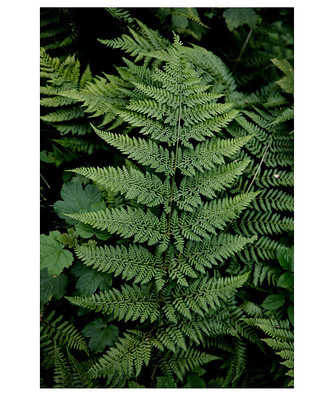
\includegraphics{images/cover.jpg}

Welcome to CSE 382 - Design Patterns \& Data Structures with Functional Programming!

In previous classes, you may have looked at design patterns and data structures that are commonly used in programming. When using functional programming, there are unique design patterns and different approaches to data structures that we need to consider. Here is the schedule for the course:

\begin{itemize}
\tightlist
\item
  Week 1 : Erlang Basics
\item
  Week 2 : Persistence
\item
  Weeks 3-7 : Design Patterns

  \begin{itemize}
  \tightlist
  \item
    Functors - Map, Filter, Fold, Unfold
  \item
    Chaining
  \item
    Currying
  \item
    Partial Applications
  \item
    Monoids
  \item
    Monads
  \item
    Streams (Lazy)
  \end{itemize}
\item
  Weeks 8-12 : Data Structures

  \begin{itemize}
  \tightlist
  \item
    Binary Search Trees
  \item
    Min Heaps
  \item
    Random Access Lists
  \item
    Tries
  \item
    Queues \& Deques
  \end{itemize}
\end{itemize}

This is a 3 credit class and there is a reading for each day (e.g Part 1 before class on Monday, Part 2 before class on Wednesday, and Part 3 before class on Friday). Each reading includes a problem set to complete. You should work on each problem set after you do each reading. During class we will cover the material in the reading with examples. The material can be complicated and fast paced so you should do the reading and attempt some of the problems before class.

We will be using Erlang in this class. If you already know Clojure, you will find that Erlang is easier to use and learn (with much fewer parentheses!). During the first week we will learn the basics of Erlang. You will learn more about Erlang as you implement the material during the course.

You will be given starting code for each problem set which you must use. You should submit all the problem sets weekly on Saturday evening to stay on track.

You can resubmit any of your work for a higher grade as many times as you want during the semester. Late work will not be penalized so you can take more time if needed to learn the material. However, submitting late work too frequently may result in getting behind which will have a negative impact on your learning and subsequent grade. During Week 13 and 14 you will have an opportunity to catch up on any missed work.

At the beginning of Week 10, you will be given an open book, open note, take-home final exam which will be due on the last day of the semester. The final exam will assess your understanding of principles taught during the course.

Your grade will be composed of 80\% for the weekly problem sets and 20\% for the final exam.

Attendance to class is highly encouraged. If you miss no more than 3 days during the semester (excluding during Week 14), you will receive a 5\% bonus on your final grade.

Office hours and contact information for this semester will be put in an I-Learn announcement.

Useful websites that would be good to bookmark:

\begin{itemize}
\item
  Erlang Book: \url{https://learning.oreilly.com/library/view/programming-erlang-2nd/9781941222454/}
\item
  CSE 121e (Erlang): \url{https://byui-cse.github.io/cse121e-course/}
\item
  Erlang Reference: \url{https://erlangbyexample.org/}
\end{itemize}

\(\nonumber\)
\href{http://creativecommons.org/licenses/by/4.0/}{
\includegraphics{images/cc-88x31.png}}

\hypertarget{erlang}{%
\chapter{Erlang}\label{erlang}}

In this course we will be using the Erlang programming language. The material that we will cover could be implemented in many different langauges. Erlang will allow us to use less code to explore the design patterns and data structures. If you haven't learned Erlang before, the two sections below will help you to quickly learn the language. As the course progresses, you will find that the implementation of future problem sets will improve your Erlang skills.

\hypertarget{quick-erlang-primer}{%
\section{Quick Erlang Primer}\label{quick-erlang-primer}}

This tutorial is not meant to provide complete coverage of the Erlang language. You are encouraged to use the Erlang references you bookmarked as needed throughout the semester.

When writing code in Erlang, you will put your code into a \texttt{.erl} file. Each Erlang file will include a \texttt{-module} and an \texttt{-export} tag. If I create a file called \texttt{learn\_erlang.erl}, then I would create the following file:

\begin{Shaded}
\begin{Highlighting}[]
\KeywordTok{{-}module}\FunctionTok{(}\CharTok{learn\_erlang}\FunctionTok{).}
\KeywordTok{{-}export}\FunctionTok{([]).}

\CommentTok{\% Put my functions here}
\end{Highlighting}
\end{Shaded}

The \texttt{-export} tag is used to list all functions that can be run externally. Functions are written in the format of \texttt{name(Parameters)\ \ -\textgreater{}\ expressions.} Note that parameters and variables always start with an uppercase letter. Functions and atoms (which are labels without values) are always lowercase.

\begin{Shaded}
\begin{Highlighting}[]
\KeywordTok{{-}module}\FunctionTok{(}\CharTok{learn\_erlang}\FunctionTok{).}
\KeywordTok{{-}export}\FunctionTok{([}\CharTok{hello}\OperatorTok{/}\DecValTok{0}\FunctionTok{,} \CharTok{average}\OperatorTok{/}\DecValTok{2}\FunctionTok{]).}

\FunctionTok{hello()} \OperatorTok{{-}\textgreater{}} \FunctionTok{io:format(}\StringTok{"Hello World!\textasciitilde{}n"}\FunctionTok{).}

\FunctionTok{average(}\VariableTok{Number1}\FunctionTok{,} \VariableTok{Number2}\FunctionTok{)} \OperatorTok{{-}\textgreater{}} \FunctionTok{(}\VariableTok{Number1}\OperatorTok{+}\VariableTok{Number2}\FunctionTok{)} \OperatorTok{/} \DecValTok{2}\FunctionTok{.}
\end{Highlighting}
\end{Shaded}

The \texttt{-export} tag shows the number of parameters (or the arity) of the function. Notice that each function ends with a period. To run the functions, execute the \texttt{erl} shell command from a terminal.

\begin{Shaded}
\begin{Highlighting}[]
\NormalTok{Eshell V12.0  (abort with \^{}G)}
\NormalTok{1\textgreater{} c(learn\_erlang).}
\NormalTok{\{ok,learn\_erlang\}}
\NormalTok{2\textgreater{} learn\_erlang:average(10,20).}
\NormalTok{15}
\end{Highlighting}
\end{Shaded}

The \texttt{c} command will compile a module. To run a function, type \texttt{module\_name:function\_name(parameters).} Notice the need to put the period just like in your code file.

\begin{Shaded}
\begin{Highlighting}[]
\FunctionTok{slope(}\VariableTok{X1}\FunctionTok{,} \VariableTok{Y1}\FunctionTok{,} \VariableTok{X2}\FunctionTok{,} \VariableTok{Y2}\FunctionTok{)} \OperatorTok{{-}\textgreater{}}
   \VariableTok{Delta\_X} \OperatorTok{=} \VariableTok{X2} \OperatorTok{{-}} \VariableTok{X1}\FunctionTok{,}
   \VariableTok{Delta\_Y} \OperatorTok{=} \VariableTok{Y2} \OperatorTok{{-}} \VariableTok{Y1}\FunctionTok{,}
   \VariableTok{Delta\_Y} \OperatorTok{/} \VariableTok{Delta\_X}\FunctionTok{.}
\end{Highlighting}
\end{Shaded}

In the \texttt{slope} function, multiple expressions are used for a slightly more complicated function. Commas are used to separate expressions in the function with a final period at the end. The last expression represents the result of the function.

\begin{Shaded}
\begin{Highlighting}[]
\FunctionTok{add(}\VariableTok{N1}\FunctionTok{,} \VariableTok{N2}\FunctionTok{)} \OperatorTok{{-}\textgreater{}} \VariableTok{N1} \OperatorTok{+} \VariableTok{N2}\FunctionTok{.}
\FunctionTok{add(}\VariableTok{N1}\FunctionTok{,} \VariableTok{N2}\FunctionTok{,} \VariableTok{N3}\FunctionTok{)} \OperatorTok{{-}\textgreater{}} \VariableTok{N1} \OperatorTok{+} \VariableTok{N2} \OperatorTok{+} \VariableTok{N3}\FunctionTok{.}
\FunctionTok{add(}\VariableTok{N1}\FunctionTok{,} \VariableTok{N2}\FunctionTok{,} \VariableTok{N3}\FunctionTok{,} \VariableTok{N4}\FunctionTok{)} \OperatorTok{{-}\textgreater{}} \VariableTok{N1} \OperatorTok{+} \VariableTok{N2} \OperatorTok{+} \VariableTok{N3} \OperatorTok{+} \VariableTok{N4}\FunctionTok{.}
\end{Highlighting}
\end{Shaded}

The function \texttt{add} exists with different arities which is why we write each one as a separate function separated by periods.

\begin{Shaded}
\begin{Highlighting}[]
\FunctionTok{divide(}\VariableTok{\_N1}\FunctionTok{,} \DecValTok{0}\FunctionTok{)} \OperatorTok{{-}\textgreater{}} \DecValTok{0}\FunctionTok{;}
\FunctionTok{divide(}\VariableTok{N1}\FunctionTok{,} \VariableTok{N2}\FunctionTok{)} \OperatorTok{{-}\textgreater{}} \VariableTok{N1} \OperatorTok{/} \VariableTok{N2}\FunctionTok{.}
\end{Highlighting}
\end{Shaded}

In the function \texttt{divide}, we have only arity 2 but we have two different scenarios or clauses. Each clause is separated by semicolons and is evaluated in order until a match is found. If we divide by 0, then the first clause will run. If we divide by non-zero, then the second clause will run.

In the \texttt{divide} function, also note that the first clause did not need to use \texttt{N1} in the expression. Unused parameters in Erlang are prefixed with an underscore.

\begin{Shaded}
\begin{Highlighting}[]
\FunctionTok{letter\_grade(}\VariableTok{Grade}\FunctionTok{)} \CharTok{when} \VariableTok{Grade} \OperatorTok{\textgreater{}=} \DecValTok{90} \OperatorTok{{-}\textgreater{}} \StringTok{"A"}\FunctionTok{;}
\FunctionTok{letter\_grade(}\VariableTok{Grade}\FunctionTok{)} \CharTok{when} \VariableTok{Grade} \OperatorTok{\textgreater{}=} \DecValTok{80} \OperatorTok{{-}\textgreater{}} \StringTok{"B"}\FunctionTok{;}
\FunctionTok{letter\_grade(}\VariableTok{Grade}\FunctionTok{)} \CharTok{when} \VariableTok{Grade} \OperatorTok{\textgreater{}=} \DecValTok{70} \OperatorTok{{-}\textgreater{}} \StringTok{"C"}\FunctionTok{;}
\FunctionTok{letter\_grade(}\VariableTok{\_Grade}\FunctionTok{)} \OperatorTok{{-}\textgreater{}} \StringTok{"F"}\FunctionTok{.}
\end{Highlighting}
\end{Shaded}

The \texttt{when} keyword is called a guard and can be used with clauses. Basic Boolean logic can be done with a guard. For more complicated logic, a \texttt{case} statement can be used which will be seen later.

\begin{Shaded}
\begin{Highlighting}[]
\FunctionTok{factorial(}\VariableTok{N}\FunctionTok{)} \CharTok{when} \VariableTok{N} \OperatorTok{=\textless{}} \DecValTok{1} \OperatorTok{{-}\textgreater{}} \DecValTok{1}\FunctionTok{;}
\FunctionTok{factorial(}\VariableTok{N}\FunctionTok{)} \OperatorTok{{-}\textgreater{}} \VariableTok{N} \OperatorTok{*} \FunctionTok{factorial(}\VariableTok{N}\OperatorTok{{-}}\DecValTok{1}\FunctionTok{).}
\end{Highlighting}
\end{Shaded}

With the understanding of clauses, we can implement recursive solutions. In this example, the base case for \texttt{factorial} is represented by the first clause (notice the \texttt{=\textless{}} syntax) and recursion is used in the second clause. The first clauses could have been rewritten without a guard if we didn't worry about negative number as: \texttt{factorial(0)\ -\textgreater{}\ 1;} We call this method of recursion ``body recursion'' because there are operations (multiply by \texttt{N}) outside of the recursive call.

\begin{Shaded}
\begin{Highlighting}[]
\FunctionTok{factorial(}\VariableTok{N}\FunctionTok{)} \OperatorTok{{-}\textgreater{}} \FunctionTok{factorial(}\VariableTok{N}\FunctionTok{,} \DecValTok{1}\FunctionTok{).}
\FunctionTok{factorial(}\DecValTok{0}\FunctionTok{,} \VariableTok{Result}\FunctionTok{)} \OperatorTok{{-}\textgreater{}} \VariableTok{Result}\FunctionTok{;}
\FunctionTok{factorial(}\VariableTok{N}\FunctionTok{,} \VariableTok{Result}\FunctionTok{)} \OperatorTok{{-}\textgreater{}} \FunctionTok{factorial(}\VariableTok{N}\OperatorTok{{-}}\DecValTok{1}\FunctionTok{,} \VariableTok{N}\OperatorTok{*}\VariableTok{Result}\FunctionTok{).}
\end{Highlighting}
\end{Shaded}

We can rewrite the same \texttt{factorial} function in what is called ``tail recursion'' format. In this case, there is no operation outside of the recursive call. This requires that we have the \texttt{Result} parameter to keep track of the ever growing value. To support a \texttt{Result} parameter, we provide a 1-arity version of the factorial function for the user to call which initializes the product to 1. When the base case is reached (in this case N is equal to 0), then we can just return the result we have been recursively growing. In Erlang, both of these methods result in the same performance. The readability for the specific problem you are solving should determine the method you use. One might argue that the ``body recursion'' method was easier to read.

\begin{Shaded}
\begin{Highlighting}[]
\FunctionTok{encrypt(}\VariableTok{Value}\FunctionTok{,} \VariableTok{Cipher\_Function}\FunctionTok{)} \OperatorTok{{-}\textgreater{}} \VariableTok{Cipher\_Function}\FunctionTok{(}\VariableTok{Value}\FunctionTok{).}

\FunctionTok{test\_encrypt()} \OperatorTok{{-}\textgreater{}}
   \VariableTok{Cipher1} \OperatorTok{=} \KeywordTok{fun} \FunctionTok{(}\VariableTok{X}\FunctionTok{)} \OperatorTok{{-}\textgreater{}} \VariableTok{X} \OperatorTok{+} \DecValTok{1} \KeywordTok{end}\FunctionTok{,}
   \VariableTok{Cipher2} \OperatorTok{=} \KeywordTok{fun} \FunctionTok{(}\VariableTok{X}\FunctionTok{)} \OperatorTok{{-}\textgreater{}} \FunctionTok{(}\DecValTok{2} \OperatorTok{*} \VariableTok{X}\FunctionTok{)} \OperatorTok{{-}} \DecValTok{3} \KeywordTok{end}\FunctionTok{,}
   \DecValTok{11} \OperatorTok{=} \FunctionTok{encrypt(}\DecValTok{10}\FunctionTok{,} \VariableTok{Cipher1}\FunctionTok{),}
   \DecValTok{17} \OperatorTok{=} \FunctionTok{encrypt(}\DecValTok{10}\FunctionTok{,} \VariableTok{Cipher2}\FunctionTok{),}
   \FloatTok{3.0} \OperatorTok{=} \FunctionTok{encrypt(}\DecValTok{1000}\FunctionTok{,} \KeywordTok{fun} \FunctionTok{math:log10}\OperatorTok{/}\DecValTok{1}\FunctionTok{),}
   \CharTok{ok}\FunctionTok{.}
\end{Highlighting}
\end{Shaded}

In this code, the second parameter \texttt{Cipher\_Function} is a function. Common in functional programming, functions are passed and used liked they were any parameter like integers and strings. The \texttt{fun\ (parameters)\ -\textgreater{}\ expression\ end} syntax is used to define an anonymous function (often called a lambda function). The \texttt{encrypt} function expects to receive a function that takes only one parameter. The \texttt{fun\ math:log10/1} is an example of providing an existing 1-arity function.

In the \texttt{test\_encrypt} function, note that \texttt{Cipher1} and \texttt{Cipher2} variables were created. We could not change the value of \texttt{Cipher1} because all variables in Erlang are immutable.

\begin{problembox}

\textbf{Problem Set 1}

You can find the template for the problem sets in this lesson here: \href{proves/prove01.erl}{prove01.erl}

As you work on these problems (as well as all future problem sets), remember to look at the test code provided in the template. There is a separate function (e.g.~\texttt{test\_ps1}) for each problem set. This will help you to understand how these problems work. You will need to uncomment out code in the test code functions as you work through each of these problems.

\begin{enumerate}
\def\labelenumi{\arabic{enumi}.}
\tightlist
\item
  Implement the \texttt{hello} function to display ``Hello World!''.
\item
  Implement the \texttt{add} function to add two numbers.
\item
  Implement the \texttt{multiply} function three different ways each with different number of parameters (i.e.~different arity):

  \begin{itemize}
  \tightlist
  \item
    Multiply one number (not very exciting)
  \item
    Multiply two numbers
  \item
    Multiply three numbers
  \end{itemize}
\item
  Implement the \texttt{water} function that will take a temperature in Fahrenheit and return ``Frozen'', ``Gas'', or ``Liquid''. Implement this using three clauses that use the \texttt{when} guard.
\item
  Implement the \texttt{fib} function to calculate the n\textsuperscript{th} Fibonacci number. Assume the 1st and 2nd number is 1. You will need to use recursion. Recommend using body recursion.
\item
  Implement the \texttt{sum} function to add up the numbers from 0 to N. Use recursion instead of using any built in functions. Recommend using body recursion.
\item
  Create lambda functions to pass to the \texttt{plot} function. The \texttt{plot} function will create \texttt{\{X,Y\}} coordinates where \texttt{X} goes from -5 to 5 and \texttt{Y} is calculated from your lambda function. Create lambda functions for the following scenarios:

  \begin{itemize}
  \tightlist
  \item
    Function that squares the number
  \item
    Function that subtracts one from the number
  \item
    Pass the \texttt{abs/1} built-in function directly
  \item
    Function that divides the number by three and then uses the \texttt{math:floor/1} built-in function to remove the decimal.
  \end{itemize}
\end{enumerate}

\end{problembox}

\hypertarget{lists-in-erlang}{%
\section{Lists in Erlang}\label{lists-in-erlang}}

Lists are built-in to Erlang at the syntax level. During the course, we will write our own functions to work with lists and we will even re-create our own list data structure. To support those activities, we need to understand how to use the built-in list first.

\begin{Shaded}
\begin{Highlighting}[]
\FunctionTok{playing\_with\_lists()} \OperatorTok{{-}\textgreater{}}
   \VariableTok{L1} \OperatorTok{=} \FunctionTok{[}\DecValTok{1}\FunctionTok{,} \DecValTok{2}\FunctionTok{,} \DecValTok{3}\FunctionTok{,} \DecValTok{4}\FunctionTok{],}
   \CharTok{ok}\FunctionTok{.}
\end{Highlighting}
\end{Shaded}

Lists can be created using square brackets. We can use a vertical bar to access the first element of the list.

\begin{Shaded}
\begin{Highlighting}[]
\FunctionTok{playing\_with\_lists()} \OperatorTok{{-}\textgreater{}}
   \VariableTok{L1} \OperatorTok{=} \FunctionTok{[}\DecValTok{1}\FunctionTok{,} \DecValTok{2}\FunctionTok{,} \DecValTok{3}\FunctionTok{,} \DecValTok{4}\FunctionTok{],}
   \VariableTok{L2} \OperatorTok{=} \FunctionTok{[}\DecValTok{0}\FunctionTok{|}\VariableTok{L1}\FunctionTok{],}
   \FunctionTok{[}\DecValTok{0}\FunctionTok{,} \DecValTok{1}\FunctionTok{,} \DecValTok{2}\FunctionTok{,} \DecValTok{3}\FunctionTok{,} \DecValTok{4}\FunctionTok{]} \OperatorTok{=} \VariableTok{L2}\FunctionTok{,}
   \CharTok{ok}\FunctionTok{.}
\end{Highlighting}
\end{Shaded}

The \texttt{{[}0\textbar{}L1{]}} prepends the \texttt{0} in front of the \texttt{L1} list. The \texttt{{[}0,\ 1,\ 2,\ 3,\ 4{]}\ =\ L2} will attempt to pattern match L2 with the list on the left hand side. If this doesn't match, our ``test'' will fail.

\begin{Shaded}
\begin{Highlighting}[]
\FunctionTok{playing\_with\_lists()} \OperatorTok{{-}\textgreater{}}
   \VariableTok{L1} \OperatorTok{=} \FunctionTok{[}\DecValTok{1}\FunctionTok{,} \DecValTok{2}\FunctionTok{,} \DecValTok{3}\FunctionTok{,} \DecValTok{4}\FunctionTok{],}
   \FunctionTok{[}\VariableTok{A} \FunctionTok{|} \VariableTok{\_}\FunctionTok{]} \OperatorTok{=} \VariableTok{L1}\FunctionTok{,}
   \DecValTok{1} \OperatorTok{=} \VariableTok{A}\FunctionTok{,}

   \VariableTok{L2} \OperatorTok{=} \FunctionTok{[}\DecValTok{2}\FunctionTok{,} \DecValTok{4}\FunctionTok{,} \DecValTok{6}\FunctionTok{,} \DecValTok{8}\FunctionTok{],}
   \FunctionTok{[}\VariableTok{B}\FunctionTok{,} \VariableTok{C} \FunctionTok{|} \VariableTok{\_}\FunctionTok{]} \OperatorTok{=} \VariableTok{L2}\FunctionTok{,}
   \DecValTok{2} \OperatorTok{=} \VariableTok{B}\FunctionTok{,}
   \DecValTok{4} \OperatorTok{=} \VariableTok{C}\FunctionTok{,}
   \CharTok{ok}\FunctionTok{.}
\end{Highlighting}
\end{Shaded}

Pattern matching can reuse the \texttt{{[}First\textbar{}Rest{]}} format. In the example above, we can extract the first or the first several values. We can match multiple values at the front of the list using commas. Note the use of the \texttt{\_} which indicates we are ignoring the ``rest'' of the list.

\begin{Shaded}
\begin{Highlighting}[]
\FunctionTok{display\_first([}\VariableTok{First}\FunctionTok{|}\VariableTok{\_Rest}\FunctionTok{])} \OperatorTok{{-}\textgreater{}}
    \FunctionTok{io:format(}\StringTok{"\textasciitilde{}p\textasciitilde{}n"}\FunctionTok{,[}\VariableTok{First}\FunctionTok{]).}

\FunctionTok{playing\_with\_lists()} \OperatorTok{{-}\textgreater{}}
    \VariableTok{L1} \OperatorTok{=} \FunctionTok{[}\DecValTok{1}\FunctionTok{,} \DecValTok{2}\FunctionTok{,} \DecValTok{3}\FunctionTok{,} \DecValTok{4}\FunctionTok{],}
    \FunctionTok{display\_first(}\VariableTok{L1}\FunctionTok{),}   
    \CharTok{ok}\FunctionTok{.}
\end{Highlighting}
\end{Shaded}

When the list \texttt{L1} is passed to the \texttt{display\_first} function, the \texttt{{[}First\textbar{}\_Rest{]}} syntax will split the list up into the first value and the remainder of the list (the latter of which is not used in the function.

\begin{Shaded}
\begin{Highlighting}[]
\FunctionTok{display\_first([])} \OperatorTok{{-}\textgreater{}}
    \FunctionTok{io:format(}\StringTok{"EMPTY\textasciitilde{}n"}\FunctionTok{);}
\FunctionTok{display\_first([}\VariableTok{First}\FunctionTok{|}\VariableTok{\_Rest}\FunctionTok{])} \OperatorTok{{-}\textgreater{}}
    \FunctionTok{io:format(}\StringTok{"\textasciitilde{}p\textasciitilde{}n"}\FunctionTok{,[}\VariableTok{First}\FunctionTok{]).}

\FunctionTok{playing\_with\_lists()} \OperatorTok{{-}\textgreater{}}
    \VariableTok{L1} \OperatorTok{=} \FunctionTok{[}\DecValTok{1}\FunctionTok{,} \DecValTok{2}\FunctionTok{,} \DecValTok{3}\FunctionTok{,} \DecValTok{4}\FunctionTok{],}
    \FunctionTok{display\_first(}\VariableTok{L1}\FunctionTok{),}   
    \FunctionTok{display\_first([]),}
    \CharTok{ok}\FunctionTok{.}
\end{Highlighting}
\end{Shaded}

In this example, a special clause is added for the empty list. We use \texttt{{[}{]}} to represent an empty list. If we wanted to represent a list of one item, we could use \texttt{{[}One{]}}. If we wanted to represent a list of more than one item, we should use \texttt{{[}First\textbar{}Rest{]}}.

\begin{Shaded}
\begin{Highlighting}[]
\FunctionTok{display\_all([])} \OperatorTok{{-}\textgreater{}}
    \FunctionTok{io:format(}\StringTok{"end of list\textasciitilde{}n"}\FunctionTok{);}
\FunctionTok{display\_all([}\VariableTok{First}\FunctionTok{|}\VariableTok{Rest}\FunctionTok{])} \OperatorTok{{-}\textgreater{}}
    \FunctionTok{io:format(}\StringTok{"\textasciitilde{}p "}\FunctionTok{,[}\VariableTok{First}\FunctionTok{]),}
    \FunctionTok{display\_all(}\VariableTok{Rest}\FunctionTok{).}

\FunctionTok{playing\_with\_lists()} \OperatorTok{{-}\textgreater{}}
    \VariableTok{L1} \OperatorTok{=} \FunctionTok{[}\DecValTok{1}\FunctionTok{,} \DecValTok{2}\FunctionTok{,} \DecValTok{3}\FunctionTok{,} \DecValTok{4}\FunctionTok{],}
    \FunctionTok{display\_all(}\VariableTok{L1}\FunctionTok{),}   
    \FunctionTok{display\_all([]),}
    \CharTok{ok}\FunctionTok{.}
\end{Highlighting}
\end{Shaded}

In this code, we need to use the entire list to display every value. Recursion is used on the \texttt{Rest} of the list. The base case is the empty list.

\begin{Shaded}
\begin{Highlighting}[]
\FunctionTok{playing\_with\_lists()} \OperatorTok{{-}\textgreater{}}
    \VariableTok{L1} \OperatorTok{=} \FunctionTok{lists:seq(}\DecValTok{1}\FunctionTok{,}\DecValTok{10}\FunctionTok{),}
    \FunctionTok{[}\DecValTok{1}\FunctionTok{,}\DecValTok{2}\FunctionTok{,}\DecValTok{3}\FunctionTok{,}\DecValTok{4}\FunctionTok{,}\DecValTok{5}\FunctionTok{,}\DecValTok{6}\FunctionTok{,}\DecValTok{7}\FunctionTok{,}\DecValTok{8}\FunctionTok{,}\DecValTok{9}\FunctionTok{,}\DecValTok{10}\FunctionTok{]} \OperatorTok{=} \VariableTok{L1}\FunctionTok{,}
    
    \VariableTok{L2} \OperatorTok{=} \FunctionTok{[}\VariableTok{N} \FunctionTok{||} \VariableTok{N} \OperatorTok{\textless{}{-}} \FunctionTok{lists:seq(}\DecValTok{1}\FunctionTok{,}\DecValTok{10}\FunctionTok{)],}
    \FunctionTok{[}\DecValTok{1}\FunctionTok{,}\DecValTok{2}\FunctionTok{,}\DecValTok{3}\FunctionTok{,}\DecValTok{4}\FunctionTok{,}\DecValTok{5}\FunctionTok{,}\DecValTok{6}\FunctionTok{,}\DecValTok{7}\FunctionTok{,}\DecValTok{8}\FunctionTok{,}\DecValTok{9}\FunctionTok{,}\DecValTok{10}\FunctionTok{]} \OperatorTok{=} \VariableTok{L2}\FunctionTok{,}

    \VariableTok{L3} \OperatorTok{=} \FunctionTok{[}\VariableTok{N}\OperatorTok{*}\DecValTok{3} \FunctionTok{||} \VariableTok{N} \OperatorTok{\textless{}{-}} \FunctionTok{lists:seq(}\DecValTok{1}\FunctionTok{,}\DecValTok{10}\FunctionTok{)],}
    \FunctionTok{[}\DecValTok{3}\FunctionTok{,}\DecValTok{6}\FunctionTok{,}\DecValTok{9}\FunctionTok{,}\DecValTok{12}\FunctionTok{,}\DecValTok{15}\FunctionTok{,}\DecValTok{18}\FunctionTok{,}\DecValTok{21}\FunctionTok{,}\DecValTok{24}\FunctionTok{,}\DecValTok{27}\FunctionTok{,}\DecValTok{30}\FunctionTok{]} \OperatorTok{=} \VariableTok{L3}\FunctionTok{,}

    \VariableTok{L4} \OperatorTok{=} \FunctionTok{[}\VariableTok{N}\OperatorTok{*}\DecValTok{3} \FunctionTok{||} \VariableTok{N} \OperatorTok{\textless{}{-}} \FunctionTok{lists:seq(}\DecValTok{1}\FunctionTok{,}\DecValTok{10}\FunctionTok{),} \VariableTok{N} \OperatorTok{rem} \DecValTok{2} \OperatorTok{==} \DecValTok{0}\FunctionTok{],}
    \FunctionTok{[}\DecValTok{6}\FunctionTok{,}\DecValTok{12}\FunctionTok{,}\DecValTok{18}\FunctionTok{,}\DecValTok{24}\FunctionTok{,}\DecValTok{30}\FunctionTok{]} \OperatorTok{=} \VariableTok{L4}\FunctionTok{,}
    
    \CharTok{ok}\FunctionTok{.}
\end{Highlighting}
\end{Shaded}

There are multiple ways to create lists. The \texttt{lists:seq} function will create numbers in a list from the range specified. The other method is the list comprehension. The syntax for the list comprehension is: \texttt{{[}expression\ \textbar{}\textbar{}\ generator,\ filter{]}} The \texttt{generator} is written with a \texttt{\textless{}-} and provides a source list. The \texttt{expression} uses the generated number to add to the list. The optional \texttt{filter} is used to determine which generated values should be used to generate the list. In the last example, the \texttt{rem} operator (often called modulo) is used to include only even numbers before tripling them.

\begin{problembox}

\textbf{Problem Set 2}

\begin{enumerate}
\def\labelenumi{\arabic{enumi}.}
\tightlist
\item
  Write a \texttt{stack\_push} function that treats the list as a stack (LIFO - Last In First Out). The \texttt{stack\_push} function will take two parameters, the \texttt{Stack} (ie, a list) and a value \texttt{N}. This function should push the value \texttt{N} to the front of the \texttt{Stack}.
\item
  Write a \texttt{stack\_pop} function that returns a new stack with the first item removed. If the stack is empty, then return the empty list \texttt{{[}{]}}.
\item
  Finish the \texttt{quicksort} function provided to you in the starting code. The algorithm for quicksort is to first pick a position in the list (in our case we will pick the first number) and call it our pivot. We will then recursively call \texttt{quicksort} on all of the numbers less than the pivot and then call quicksort on all of the numbers greater than or equal to the pivot. The correct sorted list is then the concatenation (\texttt{++}) of the following 3 lists: \texttt{{[}sorted\ list\ of\ numbers\ less\ than\ the\ pivot{]}\ ++\ {[}the\ one\ pivot{]}\ ++\ {[}sorted\ list\ of\ numbers\ greater\ than\ or\ equal\ to\ the\ pivot{]}}. The code is setup already but you need to write list comprehensions for creating:

  \begin{itemize}
  \tightlist
  \item
    A sublist containing all numbers in the list less than the pivot (first number in the list) which will be passed to the \texttt{quicksort} function.
  \item
    A sublist containing all numbers in the list greater than or equal to the pivot (first number in the list) which will be passed to the \texttt{quicksort} function.
  \end{itemize}
\end{enumerate}

\end{problembox}

\(\nonumber\)
\(\nonumber\)
\href{http://creativecommons.org/licenses/by/4.0/}{
\includegraphics{images/cc-88x31.png}}

\hypertarget{persistence}{%
\chapter{Persistence}\label{persistence}}

When we think about data structures, we think of things that change as more things are added, modified, or removed. However, in our functional world, we are dealing with immutability. This conflict causes us to learn about persistence. This week we will explore persistence with the common list.

\hypertarget{persistence-in-lists}{%
\section{Persistence in Lists}\label{persistence-in-lists}}

The lists that we are going to look at early in this course are actually linked lists. We will explore an indexed version when we look at Random Access Lists later on. Lets consider the list below that already has five elements within it.

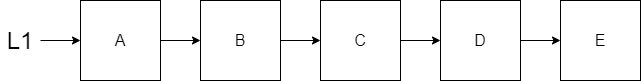
\includegraphics{images/FiveElementList.drawio.png}

Note that we have a variable \texttt{L1} that contains a reference to the first node in the list and each node in the list contains a reference to the next node. If we want to add a new node to the front of this list, we have to do it without violating the immutability rule. When we add the new node, we are creating a new list. Notice that \texttt{L2} below points to the new node we have created. However, since the remaining list doesn't need to change, we just connect the new node to the original \texttt{L1}. Since we get to reuse the entire list, the performance for prepending to the front is only O(1).

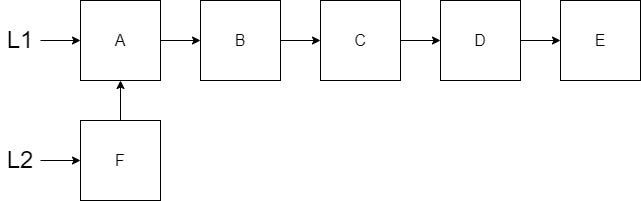
\includegraphics{images/FiveElementListPrepend.drawio.png}

Notice we have persisted the original list and created the new list by reusing what we originally had. This is what we mean be persistent data structures.

The code for this \texttt{prepend} operation does not require any recursion.

\begin{Shaded}
\begin{Highlighting}[]
\FunctionTok{prepend(}\VariableTok{List}\FunctionTok{,} \VariableTok{Value}\FunctionTok{)} \OperatorTok{{-}\textgreater{}} \FunctionTok{[}\VariableTok{Value}\FunctionTok{|}\VariableTok{List}\FunctionTok{].}
\end{Highlighting}
\end{Shaded}

Let's consider the situation where we want to append a new node to the end of the list. Looking at our original four item list, how do we add a new item to the end. We will need to create a new list \texttt{L3} and try to reuse as much as possible. However, since we are adding the new node to the end, this will cause us to not have any reuse.

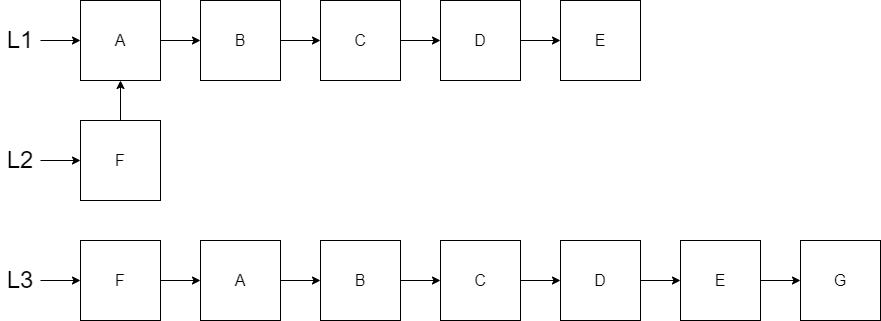
\includegraphics{images/FiveElementListAppend.drawio.png}

Notice in the picture above, the last node in the original list has to change because it needs to reference the new node instead of referencing nothing. This is a change so a new node is needed. The original last node is persisted as part of \texttt{L1} and \texttt{L2}.

The code for this \texttt{append} function requires the use of recursion. When we recurse to the end of the list (calling \texttt{append} recursively until we are left with an empty list) then we create our new node as a 1 item list.

Once we get the new node created, we return from our recursive calls and begin adding new nodes for each of the values that were in our previous list.

\begin{Shaded}
\begin{Highlighting}[]
\FunctionTok{append([],} \VariableTok{Value}\FunctionTok{)} \OperatorTok{{-}\textgreater{}} \FunctionTok{[}\VariableTok{Value}\FunctionTok{];}
\FunctionTok{append([}\VariableTok{First}\FunctionTok{|}\VariableTok{Rest}\FunctionTok{],} \VariableTok{Value}\FunctionTok{)} \OperatorTok{{-}\textgreater{}} \FunctionTok{[}\VariableTok{First} \FunctionTok{|} \FunctionTok{append(}\VariableTok{Rest}\FunctionTok{,} \VariableTok{Value}\FunctionTok{)].}
\end{Highlighting}
\end{Shaded}

When we look at the \texttt{append} function it may be concerning that there is no reuse. If all we did was call the \texttt{append} function, there would be multiple duplicates of our data all over our memory. In our programming languages, garbage collection will remove any memory that is no longer referenced by another variable. However, there is a cost for not having reuse. We have to recreate the entire list again which is O(n) performance.

In the next topic below, we will consider inserting something in the middle of our list which will cause us to reuse some of the nodes in our list.

\begin{problembox}

\textbf{Problem Set 1}

You can find the template for the problem sets in this lesson here: \href{proves/prove02.erl}{prove02.erl}

\begin{enumerate}
\def\labelenumi{\arabic{enumi}.}
\tightlist
\item
  Implement the \texttt{prepend} function as shown above.
\item
  Implement the \texttt{append} function as shown above.
\item
  To do some additional practice with lists, write a \texttt{head} function that will return the first item in the list. If the list is empty, then return the atom \texttt{nil}.
\item
  Implement a \texttt{tail} function that will return the last item in the list. The \texttt{tail} function will need to use recursion just like the \texttt{append} function. If the list is empty, then return \texttt{nil}.
\end{enumerate}

\end{problembox}

\hypertarget{more-list-persistence}{%
\section{More List Persistence}\label{more-list-persistence}}

Lets consider two more scenarios with the list and observe how persistence is maintained. First, how do we remove the first value in our list? The only thing that will be affected is our variable referencing the front of the list. In the diagram below, \texttt{L1} is the original list and \texttt{L2} is the new list with the first item removed.

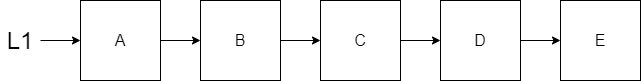
\includegraphics{images/FiveElementList.drawio.png}

Notice that \texttt{L2} is referencing the second item in the list which means all but the first original node is being reused. Both the original list and the new list persist.

Here is the code for our \texttt{remove\_first} function.

\begin{Shaded}
\begin{Highlighting}[]
\FunctionTok{remove\_first([])} \OperatorTok{{-}\textgreater{}} \FunctionTok{[];}
\FunctionTok{remove\_first([}\VariableTok{\_First}\FunctionTok{|}\VariableTok{Rest}\FunctionTok{])} \OperatorTok{{-}\textgreater{}} \VariableTok{Rest}\FunctionTok{.}
\end{Highlighting}
\end{Shaded}

Suppose we start with our original five item list \texttt{L1} again and consider inserting an item in the middle. This will be a combination of the ideas that we have seen prepending and appending to our list with respect to reuse. If we insert after index 2 (where the first element is index 0), then we will need new nodes up to index 2 and we can reuse everything after index 2.

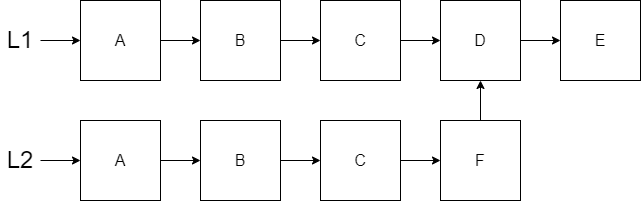
\includegraphics{images/FiveElementListInsertAt.drawio.png}

Here is the code for our \texttt{insert\_at} function. In this code, we will decrement our \texttt{Index} as we recursively search through the list. Once our \texttt{Index} reaches 0 then we know we have reached the desired location. We will then create our new node and connect it (reuse) to the remaining nodes in our original list. Notice that if our \texttt{Index} was negative then the original list is returned. For an \texttt{Index} too big, we could use the \texttt{length} function in the first clause. However, to avoid checking the length in every recursive \texttt{insert\_at} function call, we have introduced the third clause. If our \texttt{Index} is 0 in the second clause, then we know we have found the place to insert. However, if the \texttt{Index} is not 0 but the \texttt{List} is empty, then we know that our index was too big. This logic is added in the third clause.

\begin{Shaded}
\begin{Highlighting}[]
\FunctionTok{insert\_at(}\VariableTok{List}\FunctionTok{,} \VariableTok{\_Value}\FunctionTok{,} \VariableTok{Index}\FunctionTok{)} \CharTok{when} \VariableTok{Index} \OperatorTok{\textless{}} \DecValTok{0} \OperatorTok{{-}\textgreater{}} \VariableTok{List}\FunctionTok{;}
\FunctionTok{insert\_at(}\VariableTok{List}\FunctionTok{,} \VariableTok{Value}\FunctionTok{,} \DecValTok{0}\FunctionTok{)} \OperatorTok{{-}\textgreater{}} \FunctionTok{[}\VariableTok{Value} \FunctionTok{|} \VariableTok{List}\FunctionTok{];}
\FunctionTok{insert\_at([],} \VariableTok{\_Value}\FunctionTok{,} \VariableTok{\_Index}\FunctionTok{)} \OperatorTok{{-}\textgreater{}} \FunctionTok{[];}
\FunctionTok{insert\_at([}\VariableTok{First}\FunctionTok{|}\VariableTok{Rest}\FunctionTok{],} \VariableTok{Value}\FunctionTok{,} \VariableTok{Index}\FunctionTok{)} \OperatorTok{{-}\textgreater{}} \FunctionTok{[}\VariableTok{First} \FunctionTok{|} \FunctionTok{insert\_at(}\VariableTok{Rest}\FunctionTok{,} \VariableTok{Value}\FunctionTok{,} \VariableTok{Index}\OperatorTok{{-}}\DecValTok{1}\FunctionTok{)].}
\end{Highlighting}
\end{Shaded}

\begin{problembox}

\textbf{Problem Set 2}

\begin{enumerate}
\def\labelenumi{\arabic{enumi}.}
\tightlist
\item
  Implement the \texttt{remove\_first} as shown above.
\item
  Implement \texttt{insert\_at} function as shown above.
\item
  Implement a function called \texttt{remove\_last} that removes the last item in the list. If the list is empty, then return an empty list.
\item
  Implement a function called \texttt{remove\_at} like the \texttt{insert\_at} function which removes an item at a specific index. If the index is invalid, then return the original list.
\end{enumerate}

\end{problembox}

\hypertarget{specifications-and-definitions}{%
\section{Specifications and Definitions}\label{specifications-and-definitions}}

Throughout the course when we talk about a behavior, instead of immediately writing it using Erlang, we will first describe it with a specification and a definition. You may find that the our definitions and our Erlang code are similar due to the relative simplicity of the Erlang syntax. Using our definitions, you should be able to write code in any functional language.

A specification describes the interface of a function in terms of data types. Here are a list of the data types we will use in the course:

\begin{formulabox}

\begin{itemize}
\tightlist
\item
  \(integer\)
\item
  \(real\)
\item
  \(boolean\)
\item
  \(string\).
\item
  \(atom(name)\) - An atom is a label with a specified name but no value.\\
\item
  \(a\) - Represents any type
\item
  \([a]\) - List of values of any type
\item
  \(\lbrace a_1,a_2 \rbrace\) - 2 element Tuple of values of different types
\item
  \(a_1 \looparrowleft a_2\) - Dictionary (or map) defined by keys \(a_1\) and values \(a_2\).
\item
  \(\lambda\) - Function (frequently called lambda) that is passed to another function
\end{itemize}

\end{formulabox}

\(\nonumber\)

We write a specification using the \(spec\), \(::\), and \(\rightarrow\) notations. The input types are separated by spaces. An example with 3 inputs is given below. Notice that subscripts will be frequently used.

\begin{formulabox}
\(spec ~ ~ name :: input_1\_type ~ ~ input_2\_type ~ ~ input_3\_type \rightarrow output\_type.\)

\end{formulabox}

\(\nonumber\)

We can define custom types for use in our specifications by defining tuples (or records). To define a custom type, we will use the \(struct\) keyword as follows: (this example is for a tuple of size 3):

\begin{formulabox}
\(struct ~ ~ name ~ ~ \lbrace type_1:name_1, type_2:name_2, type_3:name_3 \rbrace\).

\end{formulabox}

\(\nonumber\)

In this example, there are three fields each with a type and an optional name. The keyword \(or\) will be used if there are different tuple sizes (arity) permitted in our custom type.

A definition is how the function will use the inputs to produce the output. Names will be used to give meaning to the inputs. You should refer back to the specification to understand the types. When we write definitions, we will use the following notations (excluding common ones you have seen previously such as Boolean operators and mathematical operators):

\begin{formulabox}

\begin{itemize}
\tightlist
\item
  \(=\) : Save an intermediate result into an immutable variable
\item
  \(+\), \(-\), \(*\), \(/\), \(and\), \(or\), \(>\), \(<\), \(\geq\), \(\leq\), \(==\), \(\not=\) : Commonly used operators.
\item
  \((\lambda ~ ~ input_1 ~ ~ input_2 ~ ~ input_3)\) : Call a function (in this case called \(\lambda\) with the supplied parameters. Notice that this does feel like a function call in Clojure with the parentheses.
\item
  \([]\) : Empty List
\item
  \(\lbrace \looparrowleft \rbrace\) : Empty Dictionary
\item
  \([First|Rest]\) : This splits the list where First is the first element in the list and Rest is the rest of the list.
\item
  \(List1 ++ List2\) : Combines (or concatenates) two lists together.
\item
  \(struct\_name.field\_name\) : Access a field from a custom tuple
\item
  \(nil\) - An atom that represents nothing (used sometimes for error conditions). This atom is special in that it is compatible with any type in the specification. For example, if a function was supposed to return a \([a]\), for certain conditions (like error conditions), you could return a \(nil\) in the definition.
\item
  \(\text{when} ~ ~ condition\) : Provide a guard condition on the function clause.
\item
  We will introduce many different parameter and variable names in our function definitions. Here are common ones that we will use in the examples:

  \begin{itemize}
  \tightlist
  \item
    \(List\) - A list of something
  \item
    \(Value\) - A single thing used in a computation or to be added to a data structure like a list
  \item
    \(Index\) - The index (sometimes starting at 0 or 1 depending on the problem) in a linear data structure like a list
  \item
    \(Result\) - A final answer or the current answer working towards the final answer in cases of recursion
  \item
    \(Text\) - A string that is being processed or produced
  \item
    \(Count\) - How many of something
  \item
    \(Acc\) - Represent an accumulator (something being aggregated together like adding)
  \item
    \(Curr\) - Representing the current value of something especially with counters
  \item
    \(Item\) - A single item in a collection like a list
  \item
    \(Init\) - The first or initial value of something (e.g.~an accumulator)
  \end{itemize}
\end{itemize}

\end{formulabox}

\(\nonumber\)

We write a definition using the same format as the specification but with the \(\mathit{def}\) notation in the front. Instead of data types, inputs are given names and outputs are represented as expressions that use the inputs.

\begin{formulabox}
\(de\mathit{f} ~ ~ name :: input_1 ~ ~ input_2 ~ ~ input_3 \rightarrow output\_expressions.\)

\end{formulabox}

\(\nonumber\)

If a function name exists with different number of inputs (different arity) then we will write a specification for each one. The definition for each specification may take multiple clauses. Each clause will handle a different scenario and will be separated by a semicolon. Clauses are evaluated in order. If a clause doesn't use all the inputs, then an underscore is placed in front of the input name.

Let's do some examples with our list functions. Here is the specification and definition for the \texttt{prepend} function. The prepend function took a list and a value. Therefore the specification will use inputs of \([a]\) and \(a\). The output is just a longer list so it will be \([a]\).

\begin{formulabox}
\(spec ~ ~ prepend :: [a] ~ ~ a \rightarrow [a].\)

\(de\mathit{f} ~ ~ prepend :: List ~ ~ Value \rightarrow [Value|List].\)

\end{formulabox}

\(\nonumber\)

The append function will have a similar specification but the definition will be more complicated since we had to use recursion. When you call a function in your definition, you should be the function call in parentheses. Notice that the definition uses the \([]\) and \([First|Rest]\) notation in the input to help us differentiate the two clauses.

\begin{formulabox}
\(spec ~ ~ append :: [a] ~ ~ a \rightarrow [a].\)

\(de\mathit{f} ~ ~ append :: [] ~ ~ Value \rightarrow [Value];\)

\(de\mathit{f} ~ ~ append :: [First|Rest] ~ ~ Value \rightarrow [First | (append ~ ~ Rest ~ ~ Value)].\)

\end{formulabox}

\(\nonumber\)

Let's look at the specifications and definitions for the \texttt{remove\_first} and \texttt{insert\_at} functions.

\begin{formulabox}
\(spec ~ ~ remove\_first :: [a] \rightarrow [a].\)

\(de\mathit{f} ~ ~ remove\_first :: [] \rightarrow [];\)

\(de\mathit{f} ~ ~ remove\_first::[First|Rest] \rightarrow Rest.\)

\end{formulabox}

\(\nonumber\)

In the \texttt{insert\_at} function, we need to have something called a guard. Guards are like if statements that are applied to either a clause or to part of the code within a clause. We use the phrase \(when\) in our definition to indicate a guard. The 3 clauses are evaluated in order.

\begin{formulabox}
\(spec ~ ~ insert\_at :: [a] ~ ~ a ~ ~ integer \rightarrow [a].\)

\(de\mathit{f} ~ ~ insert\_at :: List ~ ~ Value ~ ~ Index \rightarrow List ~ ~ \text{when} ~ ~ Index < 0 ~ ~ or ~ ~ Index > (length ~ ~ List);\)

\(de\mathit{f} ~ ~ insert\_at :: List ~ ~ Value ~ ~ Index \rightarrow [Value|List] ~ ~ \text{when} ~ ~ Index == 0;\)

\(de\mathit{f} ~ ~ insert\_at :: [First|Rest] ~ ~ Value ~ ~ Index \rightarrow [First|(insert\_at ~ ~ Rest ~ ~ Value ~ ~ Index-1)].\)

\end{formulabox}

\(\nonumber\)

In the definition above, we assume that there is a \texttt{length} function available.

\begin{problembox}

\textbf{Problem Set 3}

\begin{enumerate}
\def\labelenumi{\arabic{enumi}.}
\tightlist
\item
  Write the specifications and definitions for the \texttt{head}, \texttt{tail}, \texttt{removeLast}, and \texttt{removeAt} functions. You will write these in your code template as comments.
\item
  Implement a function called \texttt{backwards} (which does the same thing as the \texttt{reverse} function found in Erlang for lists). The specification and definition of this functions is shown below. Notice there are two specifications because there is a one arity function (called by the user in the test code) and a two arity function (called recursively with the result list). You will need to implement both specifications.
\end{enumerate}

\begin{formulabox}
\(spec ~ ~ backwards :: [a] \rightarrow [a].\)

\(de\mathit{f} ~ ~ backwards :: List \rightarrow (backwards ~ ~ List ~ ~ []).\)

\(spec ~ ~ backwards :: [a] ~ ~ [a] \rightarrow [a].\)

\(de\mathit{f} ~ ~ backwards :: [] ~ ~ Result \rightarrow Result;\)

\(de\mathit{f} ~ ~ backwards :: [First|Rest] ~ ~ Result \rightarrow (backwards ~ ~ Rest ~ ~ [First | Result]).\)

\end{formulabox}

\end{problembox}

\(\nonumber\)
\(\nonumber\)
\href{http://creativecommons.org/licenses/by/4.0/}{
\includegraphics{images/cc-88x31.png}}

\hypertarget{map-and-filter-functors}{%
\chapter{Map and Filter Functors}\label{map-and-filter-functors}}

The \texttt{map} and \texttt{filter} are common functions that are available in programming languages to simplify the process of processing a loop. Frequently also simplified with a list comprehension syntax, these functions provide an introduction to a very common subset of functions called functors.

\hypertarget{functors-and-map}{%
\section{Functors and Map}\label{functors-and-map}}

A functor is a mathematical term used in the field of category theory. The concept is that a functor is something that can convert from one ``category'' to another ``category''. In computer science, we consider these ``categories'' to be data types. The most common conversion involves the list. The \texttt{map} and \texttt{filter} that we use this week convert from a list to another list. The \texttt{fold} and \texttt{unfold} that we learn about next week convert from a list to a single result (and vice versa).

Let's consider the \texttt{map} function first. The \texttt{map} converts a list to another list using a lambda function. The lambda function. defines how to convert each item in the original list to an item in the result list.

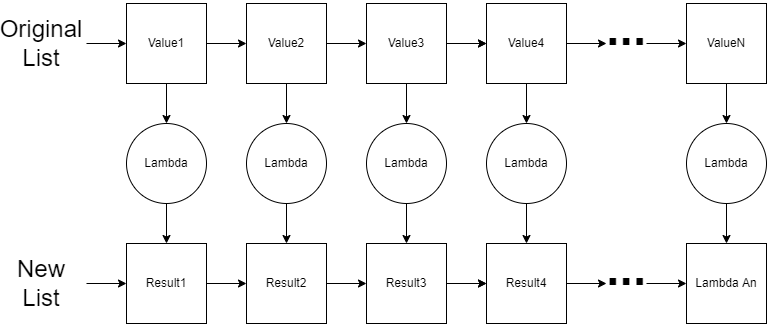
\includegraphics{images/map.drawio.png}

If I wanted to double all the values in the list, I would use the following lambda function:

\begin{formulabox}
\(spec ~ ~ \lambda : : a \rightarrow a.\)

\(de\mathit{f} ~ ~ \lambda :: Value \rightarrow Value * 2.\)

\end{formulabox}

\(\nonumber\)

If I wanted to square of all values in the list, I would use the following lambda function

\begin{formulabox}
\(spec ~ ~ \lambda :: a \rightarrow a.\)

\(de\mathit{f} ~ ~ \lambda :: Value \rightarrow Value * Value.\)

\end{formulabox}

\(\nonumber\)

If I wanted to convert a list of strings to a list of string lengths, the lambda function would be (assuming you have a function called \texttt{length}):

\begin{formulabox}
\(spec ~ ~ \lambda :: string \rightarrow integer.\)

\(de\mathit{f} ~ ~ \lambda :: Text ~ ~ \rightarrow (length ~ ~ Text).\)

\end{formulabox}

\(\nonumber\)

Notice that the \texttt{map} function is expecting that the lambda always has 2 input parameters.

Here is the formal definition of the \texttt{map}:

\begin{formulabox}
\(spec ~ ~ \lambda :: a_1 \rightarrow a_2.\)

\(spec ~ ~ map :: \lambda ~ ~ [a_1]\rightarrow [a_2].\)

\(de\mathit{f} ~ ~ map :: \lambda ~ ~ [] \rightarrow [];\)

\(de\mathit{f} ~ ~ map :: \lambda ~ ~ [First | Rest] \rightarrow [(\lambda ~ ~ First)|(map ~ ~ \lambda ~ ~ Rest)]\)

\end{formulabox}

\(\nonumber\)

First thing to notice is that \texttt{map} function does reply on the definition for \(\lambda\). Also notice the recursive nature of the \texttt{map} as it applies the lambda function to the each element one at a time starting with the first element (\(First\)). The result of calling the lambda function (\(\lambda ~ ~ First\)) becomes the new value to add to the front of the resulting list.

Consider the code implementation in Erlang below.

\begin{Shaded}
\begin{Highlighting}[]
\FunctionTok{map(}\VariableTok{\_Lambda}\FunctionTok{,} \FunctionTok{[])} \OperatorTok{{-}\textgreater{}} \FunctionTok{[];}
\FunctionTok{map(}\VariableTok{Lambda}\FunctionTok{,} \FunctionTok{[}\VariableTok{First}\FunctionTok{|}\VariableTok{Rest}\FunctionTok{])} \OperatorTok{{-}\textgreater{}} \FunctionTok{[}\VariableTok{Lambda}\FunctionTok{(}\VariableTok{First}\FunctionTok{)|map(}\VariableTok{Lambda}\FunctionTok{,} \VariableTok{Rest}\FunctionTok{)].}
\end{Highlighting}
\end{Shaded}

Functors in programming will frequently use a lambda function to allow us to write more generalized and abstract functions like \texttt{map}. Notice that the \texttt{map} function doesn't know what the lambda will do except that it is a lambda that converts one value to another value. Note that Erlang also has a built-in function \texttt{lists:map}.

\begin{problembox}

\textbf{Problem Set 1}

You can find the template for the problem sets in this lesson here: \href{proves/prove03.erl}{prove03.erl}

\begin{enumerate}
\def\labelenumi{\arabic{enumi}.}
\tightlist
\item
  Implement the \texttt{map} function described above and write test code to convert a list of measurements in inches to a list of measurements in centimeters. Use the formula \(1 in = 2.54 cm.\)
\item
  Using the \texttt{map} function you wrote, use a simple cipher to encrypt a list of characters. The simple cipher should shift all characters by 1 per the \href{https://www.asciitable.com/}{ASCII table} . For example, ``PASSWORD'' should be ``QBTTXPSE''. In Erlang, a string is represented as a list of characters. Therefore, you can list notation with strings. Additionally, each character is treated as a number as shown in the ASCII table which means you can add numbers to letters.
\item
  Rewrite the \texttt{map} function using a list comprehension and test it with your cipher test code. Call the new function \texttt{map\_2}.
\end{enumerate}

\end{problembox}

\hypertarget{filter}{%
\section{Filter}\label{filter}}

The \texttt{filter} function is a functor that converts from a list to a list just like the \texttt{map} function. However, the lambda function used by \texttt{filter} is intended to return a boolean result that will be used to determine if the value in the original list will be included in the new list.

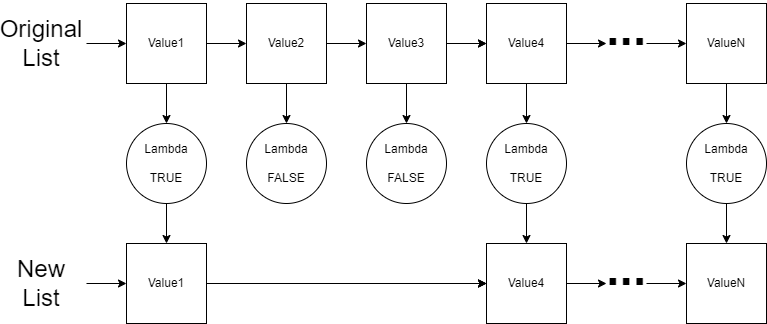
\includegraphics{images/filter.drawio.png}

If I wanted to include only even number values in my list, then the lambda function would be as follows:

\begin{formulabox}
\(spec ~ ~ \lambda :: integer \rightarrow boolean\)

\(de\mathit{f} ~ ~ \lambda :: Value \rightarrow Value ~ ~ mod ~ ~ 2 == 0.\)

\end{formulabox}

\(\nonumber\)

If I wanted to include only three digit numbers, then the lambda function would be:

\begin{formulabox}
\(spec ~ ~ \lambda :: integer \rightarrow boolean\)

\(de\mathit{f} ~ ~ \lambda :: Value \rightarrow Value \ge 100 ~ ~ and ~ ~ Value \le 999.\)

\end{formulabox}

\(\nonumber\)

In both of these examples above, the lambda function is expected to return a boolean condition. If it returns true, then the item will be included in the resulting list.

The formal definition of the \texttt{filter} is given below. The implementation is left for an exercise. Note that Erlang does have a built-in function called \texttt{lists:filter}.

\begin{formulabox}
\(spec ~ ~ \lambda :: a \rightarrow boolean\)

\(spec ~ ~ \mathit{filter} :: \lambda ~ ~ [a] \rightarrow [a].\)

\(de\mathit{f} ~ ~ \mathit{filter} :: \lambda ~ ~ [] \rightarrow [];\)

\(de\mathit{f} ~ ~ \mathit{filter} :: \lambda ~ ~ [First | Rest] \rightarrow [First|(\mathit{filter} ~ ~ \lambda ~ ~ Rest)] ~ ~ \text{when} ~ ~ (\lambda ~ ~ First) == true;\)

\(de\mathit{f} ~ ~ \mathit{filter} :: \lambda ~ ~ [First | Rest] \rightarrow (\mathit{filter} ~ ~ \lambda ~ ~ Rest).\)

\end{formulabox}

\(\nonumber\)

In Erlang, we are limited in what we can put in a \texttt{when} guard including boolean operations and a limited subset of built-in functions. When we need to compare a computed result (in the case of the \texttt{filter} we need to run the lambda function and consider the result), you can use a \texttt{case} statement. With a \texttt{case} statement, you can use \texttt{\_Else} to represent the default or otherwise case.

\begin{Shaded}
\begin{Highlighting}[]
\FunctionTok{did\_it\_work(}\VariableTok{Number}\FunctionTok{)} \OperatorTok{{-}\textgreater{}}
   \VariableTok{Result} \OperatorTok{=} \FunctionTok{process\_it(}\VariableTok{Number}\FunctionTok{),}
   \KeywordTok{case} \VariableTok{Result} \KeywordTok{of}
      \DecValTok{42} \OperatorTok{{-}\textgreater{}} \FunctionTok{do\_something(}\VariableTok{Number}\FunctionTok{);}
      \VariableTok{\_Else} \OperatorTok{{-}\textgreater{}} \FunctionTok{do\_something\_else(}\VariableTok{Number}\FunctionTok{)}
   \KeywordTok{end}\FunctionTok{.}

\FunctionTok{try\_something\_else(}\VariableTok{Number}\FunctionTok{)} \OperatorTok{{-}\textgreater{}}
   \VariableTok{Result} \OperatorTok{=} \FunctionTok{process\_it(}\VariableTok{Number}\FunctionTok{),}
   \KeywordTok{case} \VariableTok{Number} \OperatorTok{\textgreater{}} \DecValTok{42} \KeywordTok{of}
      \CharTok{true} \OperatorTok{{-}\textgreater{}} \FunctionTok{do\_something(}\VariableTok{Number}\FunctionTok{);}
      \VariableTok{\_Else} \OperatorTok{{-}\textgreater{}} \FunctionTok{do\_something\_else(}\VariableTok{Number}\FunctionTok{)}
   \KeywordTok{end}\FunctionTok{.}
\end{Highlighting}
\end{Shaded}

Note that Erlang provides this function as a built-in function called \texttt{lists:filter}.

\begin{problembox}

\textbf{Problem Set 2}

\begin{enumerate}
\def\labelenumi{\arabic{enumi}.}
\tightlist
\item
  Implement the \texttt{filter} function in Erlang. Use a \texttt{case} block to determine whether an item in the list should be included. Test the \texttt{filter} to get a list of even numbers from a list using the lambda described in the reading.
\item
  Rewrite the \texttt{filter} function so that it uses a list comprehension instead of using the \texttt{case}. Test the new function with the same lambda function in the previous problem. Call the new function \texttt{filter\_2}.
\item
  Use the \texttt{filter} functions you wrote to filter a list of temperatures (in Celsius) that will support liquid water (as opposed to frozen ice or boiling steam).
\item
  Use the \texttt{filter} function you wrote to filter a list of result strings that started with the prefix ``ERROR:''. Consider using the \texttt{string:prefix} function to solve this problem.
\end{enumerate}

\end{problembox}

\hypertarget{functor-properties}{%
\section{Functor Properties}\label{functor-properties}}

Our \texttt{map} and \texttt{filter} functions are special in that satisfy the following properties which apply in mathematics to functors:

\begin{enumerate}
\def\labelenumi{\arabic{enumi}.}
\tightlist
\item
  Identity - The functor must be able to convert back to itself. In math, 1 is an identity for multiplication and 0 is an identify for addition.\\
\item
  Distributive - The functor must be able to behave with the distributive property. In math, if I had a functor \(f\) and two other functions \(g\) and \(h\), then the following must be true: \(f(g(h)) = f(g)(f(h))\). This is frequently written using composition notation: \(f(g \circ h) = f(g) \circ f(h)\). This means that I can apply my function \(f\) to either \(g\) and \(h\) combined or I can apply function \(f\) separately to \(g\) and \(h\) and then combine the results.
\end{enumerate}

In the examples below, we will observe how these mathematical properties are satisfied by \texttt{map} and \texttt{filter}. The identity property requires us to find a \(\lambda\) that will result in no changes to our original list.

\begin{formulabox}
\(spec ~ ~ \lambda :: a \rightarrow a.\)

\(de\mathit{f} ~ ~ \lambda :: Value \rightarrow Value.\)

\end{formulabox}

\(\nonumber\)

Here is the code that demonstrates that identity principle using the \texttt{map} written earlier:

\begin{Shaded}
\begin{Highlighting}[]
\FunctionTok{[}\DecValTok{1}\FunctionTok{,}\DecValTok{2}\FunctionTok{,}\DecValTok{3}\FunctionTok{,}\DecValTok{4}\FunctionTok{]} \OperatorTok{=} \FunctionTok{map(}\KeywordTok{fun}\FunctionTok{(}\VariableTok{Value}\FunctionTok{)} \OperatorTok{{-}\textgreater{}} \VariableTok{Value} \KeywordTok{end}\FunctionTok{,} \FunctionTok{[}\DecValTok{1}\FunctionTok{,}\DecValTok{2}\FunctionTok{,}\DecValTok{3}\FunctionTok{,}\DecValTok{4}\FunctionTok{]),}
\end{Highlighting}
\end{Shaded}

Now lets consider the second rule of functors. Does the distributive property hold? In the formula \(f(g \circ h) = f(g) \circ f(h)\), we will use the \texttt{map} function as our functor \(f\). The \(g\) and the \(h\) will be separate lambda functions which are randomly selected for demonstration purposes.

\begin{formulabox}
\(spec ~ ~ \lambda_g :: a \rightarrow a.\)

\(de\mathit{f} ~ ~ \lambda_g :: Value \rightarrow 2 * Value.\)

\(spec ~ ~ \lambda_h:: a \rightarrow a.\)

\(de\mathit{f} ~ ~ \lambda_h :: Value \rightarrow (Value*Value) - 1.\)

\end{formulabox}

\(\nonumber\)

In the following code, we will implement both sides of the distributive property to see if it holds true using a simple list of numbers.

\begin{Shaded}
\begin{Highlighting}[]
\VariableTok{G} \OperatorTok{=} \KeywordTok{fun}\FunctionTok{(}\VariableTok{Value}\FunctionTok{)} \OperatorTok{{-}\textgreater{}} \DecValTok{2} \OperatorTok{*} \VariableTok{Value} \KeywordTok{end}\FunctionTok{,}
\VariableTok{H} \OperatorTok{=} \KeywordTok{fun}\FunctionTok{(}\VariableTok{Value}\FunctionTok{)} \OperatorTok{{-}\textgreater{}} \FunctionTok{(}\VariableTok{Value} \OperatorTok{*} \VariableTok{Value}\FunctionTok{)} \OperatorTok{{-}} \DecValTok{1} \KeywordTok{end}\FunctionTok{,}

\CommentTok{\% Left Side of Distributive Property}
\VariableTok{G\_H} \OperatorTok{=} \KeywordTok{fun}\FunctionTok{(}\VariableTok{Value}\FunctionTok{)} \OperatorTok{{-}\textgreater{}} \VariableTok{G}\FunctionTok{(}\VariableTok{H}\FunctionTok{(}\VariableTok{Value}\FunctionTok{))} \KeywordTok{end}\FunctionTok{,}
\FunctionTok{[}\DecValTok{0}\FunctionTok{,}\DecValTok{6}\FunctionTok{,}\DecValTok{16}\FunctionTok{,}\DecValTok{30}\FunctionTok{]} \OperatorTok{=} \FunctionTok{map(}\VariableTok{G\_H}\FunctionTok{,} \FunctionTok{[}\DecValTok{1}\FunctionTok{,}\DecValTok{2}\FunctionTok{,}\DecValTok{3}\FunctionTok{,}\DecValTok{4}\FunctionTok{]),}

\CommentTok{\% Right Side of Distributive Property}
\FunctionTok{[}\DecValTok{0}\FunctionTok{,}\DecValTok{6}\FunctionTok{,}\DecValTok{16}\FunctionTok{,}\DecValTok{30}\FunctionTok{]} \OperatorTok{=} \FunctionTok{map(}\VariableTok{G}\FunctionTok{,} \FunctionTok{map(}\VariableTok{H}\FunctionTok{,} \FunctionTok{[}\DecValTok{1}\FunctionTok{,}\DecValTok{2}\FunctionTok{,}\DecValTok{3}\FunctionTok{,}\DecValTok{4}\FunctionTok{])),}
\end{Highlighting}
\end{Shaded}

While understanding the properties of functors is educational, the way the code is written in the two examples above is more instructive. Notice the creation of the \texttt{G\_H} function which is the composition of two functions. Also note that the this was needed because the \texttt{map} function requires a lambda with only one parameter. As you study the code above, notice how the \texttt{map} functions were combined together in the ``Right Side'' case. We call this ``chaining'' which we will learn about next week.

Demonstrations of these two properties of functors for the \texttt{filter} function is left as an exercise.

\begin{problembox}

\textbf{Problem Set 3}

\begin{enumerate}
\def\labelenumi{\arabic{enumi}.}
\tightlist
\item
  Write code in Erlang to demonstrate the identity property for the \texttt{filter} functor. Reuse the \texttt{filter} function you wrote earlier.
\item
  Write code in Erlang to demonstrate the distributive property for the \texttt{filter} function. Reuse the \texttt{filter} function you wrote earlier. You will have to come up with your own appropriate \texttt{G} and \texttt{H} lambda functions in your demonstration. Remember that the lambda functions for \texttt{filter} expect to return boolean. In other words, when you demonstrate the distributive property, you will be composing (or chaining) boolean conditions together using the \texttt{and} operator.
\end{enumerate}

\end{problembox}

\(\nonumber\)
\(\nonumber\)
\href{http://creativecommons.org/licenses/by/4.0/}{
\includegraphics{images/cc-88x31.png}}

\hypertarget{fold-and-unfold-functors}{%
\chapter{Fold and Unfold Functors}\label{fold-and-unfold-functors}}

The \texttt{fold} and \texttt{unfold} are part of the common functor design patterns. A \texttt{fold} will convert from a list to a single value whereas an \texttt{unfold} will convert from a single value and a list.

\hypertarget{fold}{%
\section{Fold}\label{fold}}

Just like the \texttt{map} and \texttt{filter} patterns, we will use a lambda function to define what we want to do with each item of the list. Unlike the \texttt{map} and \texttt{filter}, we will not apply the lambda function to determine what to put in the resulting list. Instead (in the case of \texttt{fold}) we will use the lambda function to determine how each item in our list contributes to the one single value result. The lambda function is used to combine all the values in the list.

If I have a list of numbers \texttt{{[}1\ 2\ 3\ 4\ 5{]}} that I wanted to add, then a lambda function would take each number (\(Value\)) and add it to an accumulator (\(Acc\)):

\begin{formulabox}
\(spec ~ ~ \lambda :: real ~ ~ real \rightarrow real.\)

\(de\mathit{f} ~ ~ \lambda :: Value ~ ~ Acc \rightarrow Acc + Value.\)

\end{formulabox}

\(\nonumber\)

If I wanted to add the squares of the numbers in the list, then I would want the lambda function to be

\begin{formulabox}
\(spec ~ ~ \lambda :: real ~ ~ real \rightarrow real.\)

\(de\mathit{f} ~ ~ \lambda :: Value ~ ~ Acc \rightarrow Acc + (Value * Value).\)

\end{formulabox}

\(\nonumber\)

The result of the lambda functions will be passed in as the accumulator value when we goto the next item in the list. This implies that we will need to define what the initial accumulator value should be.

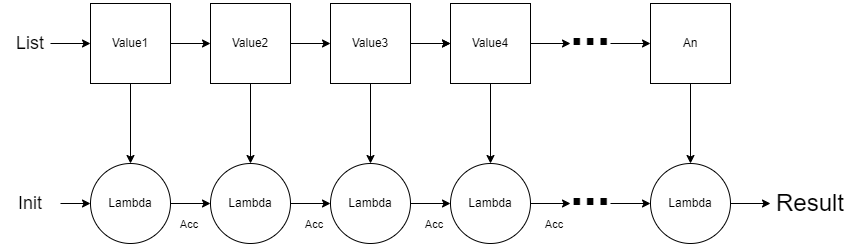
\includegraphics{images/fold.drawio.png}

Notice that the \texttt{fold} function is expecting that the lambda always has 2 input parameters where the second parameter is the accumulator. The single output of the \(\lambda\) function is the updated accumulator.

Here is the formal definition of the \texttt{fold}:

\begin{formulabox}
\(spec ~ ~ \lambda :: a_1 ~ ~ a_2 \rightarrow a_2.\)

\(spec ~ ~ \mathit{fold} :: \lambda ~ ~ a_2 ~ ~ [a_1]\rightarrow a_2.\)

\(de\mathit{f} ~ ~ \mathit{fold} :: \lambda ~ ~ Acc ~ ~ []\rightarrow Acc;\)

\(de\mathit{f} ~ ~ \mathit{fold} :: \lambda ~ ~ Acc ~ ~ [First|Rest] \rightarrow (\mathit{fold} ~ ~ \lambda ~ ~ (\lambda ~ ~ First ~ ~ Acc) ~ ~ Rest).\)

\end{formulabox}

\(\nonumber\)

Notice the recursive nature of the \texttt{fold} as it applies the lambda function to the each element one at a time starting with the first element (\(First\)). The result of calling the lambda function (\(\lambda ~ ~ First ~ ~ Acc\)) becomes the new accumulator value when \texttt{fold} is called recursively on the remainder of the list (\(Rest\)).

Consider the code implementation below.

\begin{Shaded}
\begin{Highlighting}[]
\FunctionTok{fold(}\VariableTok{\_Lambda}\FunctionTok{,} \VariableTok{Acc}\FunctionTok{,} \FunctionTok{[])} \OperatorTok{{-}\textgreater{}} \VariableTok{Acc}\FunctionTok{;}
\FunctionTok{fold(}\VariableTok{Lambda}\FunctionTok{,} \VariableTok{Acc}\FunctionTok{,} \FunctionTok{[}\VariableTok{First}\FunctionTok{|}\VariableTok{Rest}\FunctionTok{])} \OperatorTok{{-}\textgreater{}} \FunctionTok{fold(}\VariableTok{Lambda}\FunctionTok{,} \VariableTok{Lambda}\FunctionTok{(}\VariableTok{First}\FunctionTok{,} \VariableTok{Acc}\FunctionTok{),} \VariableTok{Rest}\FunctionTok{).}
\end{Highlighting}
\end{Shaded}

The initial \texttt{Acc} passed to the \texttt{fold} function represents the initial value of the accumulator. If we were summing up numbers in a list, we would expect the initial accumulator to be 0.

Note that Erlang provides this function as a built-in function called \texttt{lists:foldl} (meaning fold left).

\begin{problembox}

\textbf{Problem Set 1}

You can find the template for the problem sets in this lesson here: \href{proves/prove04.erl}{prove04.erl}

\begin{enumerate}
\def\labelenumi{\arabic{enumi}.}
\tightlist
\item
  Implement the the \texttt{fold} code and use the lambda examples above to sum a list of numbers. Test code is provided for you in the starting code.
\item
  Create a lambda function to use with your \texttt{fold} function to concatenate a list of strings. Note that you can use the \texttt{++} operator to solve this problem. Test code is provided for you in the starting code.
\item
  Create a lambda function to use with your \texttt{fold} function to count the number of items in a list. Test code is provided for you in the starting code.
\item
  Create a lambda function to use with your \texttt{fold} function to reverse a list. Note that the single result that a \texttt{fold} returns can be a list if the lambda function is written properly. Test code is provided for you in the starting code.
\end{enumerate}

\end{problembox}

\hypertarget{fold-right}{%
\section{Fold Right}\label{fold-right}}

When you look at the definition of \texttt{fold} notice that the list is processed from left to right. We can define a function that goes from right to left called \texttt{foldr}. This function will require us to traverse to the end of the list before we can actually call the lambda function.

\begin{formulabox}
\(spec ~ ~ \lambda :: a_1 ~ ~ a_2 \rightarrow a_2.\)

\(spec ~ ~ \mathit{foldr} :: \lambda ~ ~ a_2 ~ ~ [a_1]\rightarrow a_2.\)

\(de\mathit{f} ~ ~ \mathit{foldr} :: \lambda ~ ~ Acc ~ ~ [] \rightarrow Acc;\)

\(de\mathit{f} ~ ~ \mathit{foldr} :: \lambda ~ ~ Acc ~ ~ [First|Rest]\rightarrow (\lambda ~ ~ First ~ ~ (\mathit{foldr} ~ ~ \lambda ~ ~ Acc ~ ~ Rest)).\)

\end{formulabox}

\(\nonumber\)

The code implementation of our function in Erlang is left for an exercise below. Erlang provides a built-in function called \texttt{lists:foldr} to perform this task.

\begin{problembox}

\textbf{Problem Set 2}

\begin{enumerate}
\def\labelenumi{\arabic{enumi}.}
\tightlist
\item
  Implement \texttt{foldr} and test it with the concatenation of a list of strings. Observe the different behavior with the left \texttt{fold}.
\end{enumerate}

\end{problembox}

\hypertarget{unfold}{%
\section{Unfold}\label{unfold}}

The \texttt{fold} design pattern is used when you want to consolidate from one larger thing to a smaller thing such as a list to a single value. If we want to go backwards, this is called an \texttt{unfold}. Note that folding and unfolding are not inversely related. For example, if I had a list of numbers \texttt{{[}2\ 5\ 3\ 1{]}} and I folded them up using a simple sum function, I would get \texttt{11}. However, if started with \texttt{11} and worked backwards, I could get a possible solution such as \texttt{{[}7\ 1\ 3\ 0{]}} which is different from our original list.

When we \texttt{unfold}, we are relying on some initial conditions to generate the next value for our list based on those initial conditions.

Suppose we wanted to generate a list of \(Count\) numbers with a value of \(Value\). We want to \texttt{unfold} our initial conditions to obtain a list of numbers. For example, if \(Count\) is 4 and \(Value\) is 6, then the \texttt{gensame} function should result in \texttt{{[}6\ 6\ 6\ 6{]}}. Here is a definition for our \texttt{gensame} function:

\begin{formulabox}
\(spec ~ ~ gensame :: integer ~ ~ real \rightarrow [real].\)

\(de\mathit{f} ~ ~ gensame :: 0 ~ ~ Value \rightarrow [];\)

\(de\mathit{f} ~ ~ gensame :: Count ~ ~ Value \rightarrow [Value | (gensame ~ ~ (Count-1) ~ ~ Value)].\)

\end{formulabox}

\(\nonumber\)

Here is the Erlang code for \texttt{gensame}:

\begin{Shaded}
\begin{Highlighting}[]
\FunctionTok{gensame(}\DecValTok{0}\FunctionTok{,} \VariableTok{\_Value}\FunctionTok{)} \OperatorTok{{-}\textgreater{}} \FunctionTok{[];}
\FunctionTok{gensame(}\VariableTok{Count}\FunctionTok{,} \VariableTok{Value}\FunctionTok{)} \OperatorTok{{-}\textgreater{}} \FunctionTok{[}\VariableTok{Value} \FunctionTok{|} \FunctionTok{gensame(}\VariableTok{Count}\OperatorTok{{-}}\DecValTok{1}\FunctionTok{,} \VariableTok{Value}\FunctionTok{)].}
\end{Highlighting}
\end{Shaded}

We could modify this function to create an increasing sequence of numbers by including an initial value (\(Init\)) and step size (\(Step\)). To accomplish this, we need to define a lambda function to calculate the next value. We will use \(Curr\) to represent the current value that started with \(Init\) and was increased by \(Step\).

For example, if we wanted a list of 5 even numbers starting at 4, then \(Count\) would be 5, \(Init\) would be 4, and our lambda would be:

\begin{formulabox}
\(spec ~ ~ \lambda :: real \rightarrow real.\)

\(de\mathit{f} ~ ~ \lambda :: Curr \rightarrow Curr + 2.\)

\end{formulabox}

\(\nonumber\)

The output of our \texttt{genincr} function would be \texttt{{[}4\ 6\ 8\ 10\ 12{]}}.

\begin{formulabox}
\(spec ~ ~ genincr :: integer ~ ~ real ~ ~ \lambda \rightarrow [real].\)

\(de\mathit{f} ~ ~ genincr :: 0 ~ ~ Curr ~ ~ \lambda \rightarrow [];\)

\(de\mathit{f} ~ ~ genincr :: Count ~ ~ Curr ~ ~ \lambda \rightarrow [Curr | (genincr ~ ~ (Count-1) ~ ~ (\lambda ~ ~ Curr) ~ ~ \lambda)].\)

\end{formulabox}

\(\nonumber\)

Looking at these two examples, we can generalize our function. Let's create a generic \texttt{unfold} function that works for more than just numbers.

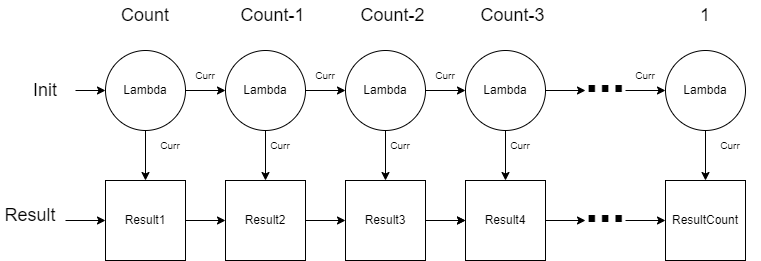
\includegraphics{images/unfold.drawio.png}

This function does not exist in the Erlang library primarily because its not generic enough. We can create an \texttt{unfold} type function that does not rely on a \texttt{Count} variable or uses a lambda function that has a different number of parameters. The specification and definition is the same as \texttt{genincr} but will have a more generalized lambda specification with no definition.

\begin{formulabox}
\(spec ~ ~ \lambda :: a \rightarrow a.\)

\end{formulabox}

\(\nonumber\)

The Erlang code for \texttt{unfold} is given below:

\begin{Shaded}
\begin{Highlighting}[]
\FunctionTok{unfold(}\DecValTok{0}\FunctionTok{,} \VariableTok{\_Curr}\FunctionTok{,} \VariableTok{\_Lambda}\FunctionTok{)} \OperatorTok{{-}\textgreater{}} \FunctionTok{[];}
\FunctionTok{unfold(}\VariableTok{Count}\FunctionTok{,} \VariableTok{Curr}\FunctionTok{,} \VariableTok{Lambda}\FunctionTok{)} \OperatorTok{{-}\textgreater{}} \FunctionTok{[}\VariableTok{Curr}\FunctionTok{|unfold(}\VariableTok{Count}\OperatorTok{{-}}\DecValTok{1}\FunctionTok{,} \VariableTok{Lambda}\FunctionTok{(}\VariableTok{Curr}\FunctionTok{),} \VariableTok{Lambda}\FunctionTok{)].}
\end{Highlighting}
\end{Shaded}

\begin{problembox}

\textbf{Problem Set 3}

\begin{enumerate}
\def\labelenumi{\arabic{enumi}.}
\tightlist
\item
  Implement the \texttt{unfold} function as described above and use it to generate an arithmetic sequence of numbers starting at 5 and ending at 30 stepping by 5 (\texttt{{[}5,\ 10,\ 15,\ 20,\ 25,\ 30{]}}).
\item
  Use the \texttt{unfold} function to generate an geometric sequence of six numbers starting at 1 with a factor of \(1/2\) (\texttt{{[}1,\ 0.5,\ 0.25,\ 0.125,\ 0.0625,\ 0.03125{]}}).
\item
  Write a function called \texttt{range} that takes in \(Start\), \(Size\), and \(Step\) parameters (in that order) and returns a list of size \(Size\) starting at \(Start\), stepping by \(Step\). Your \texttt{range} function must use the \texttt{unfold} function. For example, \texttt{range(3,5,4)} would return \texttt{{[}3,\ 7,\ 11,\ 15,\ 19{]}}. You should assume that both \(Size\) and \(Step\) are positive integers greater than 0.
\end{enumerate}

\end{problembox}

\(\nonumber\)
\(\nonumber\)
\href{http://creativecommons.org/licenses/by/4.0/}{
\includegraphics{images/cc-88x31.png}}

\hypertarget{chaining-currying-and-partial-applications}{%
\chapter{Chaining, Currying, and Partial Applications}\label{chaining-currying-and-partial-applications}}

In this lesson we will learn about three different but related design patterns. \texttt{Chaining} will consider the composition of functions. \texttt{Currying} will convert a function into multiple functions based on input parameters thus allowing you to chain the input parameters together. \texttt{Partial\ Applications} will convert a function into multiple functions based on behavior thus allowing you to execute part of the original function and reuse the result multiple times.

\hypertarget{chaining}{%
\section{Chaining}\label{chaining}}

If we need to apply multiple operations on our inputs, we can define each operation in a function and then chain them together. Chaining is the process of executing a series of functions where the output of one is used as the input for the next. Mathematically, we show chaining or composition as follows:

\begin{formulabox}
\(\mathit{f}(g(h())) = \mathit{f} \circ g \circ h\)

\end{formulabox}

\(\nonumber\)

In this example, \(h\) runs first and passes the result to function \(g\). After \(g\) runs, the result is passed to function \(\mathit{f}\).

Consider the following Erlang functions that are chained together in various ways:

\begin{Shaded}
\begin{Highlighting}[]
\FunctionTok{twice(}\VariableTok{X}\FunctionTok{)} \OperatorTok{{-}\textgreater{}} \DecValTok{2} \OperatorTok{*} \VariableTok{X}\FunctionTok{.}
\FunctionTok{square(}\VariableTok{X}\FunctionTok{)} \OperatorTok{{-}\textgreater{}} \VariableTok{X} \OperatorTok{*} \VariableTok{X}\FunctionTok{.}
\FunctionTok{third(}\VariableTok{X}\FunctionTok{)} \OperatorTok{{-}\textgreater{}} \VariableTok{X} \OperatorTok{/} \DecValTok{3}\FunctionTok{.}

\FunctionTok{test\_chain()} \OperatorTok{{-}\textgreater{}}
    \FloatTok{6.0} \OperatorTok{=} \FunctionTok{third(twice(square(}\DecValTok{3}\FunctionTok{))),}
    \FloatTok{6.0} \OperatorTok{=} \FunctionTok{twice(third(square(}\DecValTok{3}\FunctionTok{))),}
    \FloatTok{4.0} \OperatorTok{=} \FunctionTok{square(twice(third(}\DecValTok{3}\FunctionTok{))),}
    \FloatTok{2.0} \OperatorTok{=} \FunctionTok{twice(square(third(}\DecValTok{3}\FunctionTok{))),}
    \CharTok{ok}\FunctionTok{.}
\end{Highlighting}
\end{Shaded}

Note that we were able to chain the functions in all various permutations because each of the functions had a single number input and single number output.

If you think about the \texttt{map} and \texttt{filter} functions, these could be chained together because they both have a single list as an input and output. You will make this observation in the exercises below.

When we chain functions, we can also work with functions that return functions. Consider the functions \texttt{multiply\_list} and \texttt{greater\_list}:

\begin{formulabox}
\(spec ~ ~ multiply\_list :: real \rightarrow (\lambda :: [real] \rightarrow [real]).\)

\(spec ~ ~ \lambda_{map} :: real \rightarrow real.\)

\(de\mathit{f} ~ ~ multiply\_list :: Value \rightarrow (\lambda :: List \rightarrow (map ~ ~ (\lambda_{map} :: Item \rightarrow Item * Value) ~ ~ List)).\)

\end{formulabox}

\(\nonumber\)

\begin{formulabox}
\(spec ~ ~ greater\_list :: real \rightarrow (\lambda :: [real] \rightarrow [real]).\)

\(spec ~ ~ \lambda_{filter} :: real \rightarrow boolean.\)

\(de\mathit{f} ~ ~ greater\_list :: Value \rightarrow (\lambda :: List \rightarrow (\mathit{filter} ~ ~ (\lambda_{filter} :: Item \rightarrow Item > Value) ~ ~ List)).\)

\end{formulabox}

\(\nonumber\)

In these definitions, the function returns a function that does either a \texttt{map} or a \texttt{filter}. The lambda function for \texttt{map} and \texttt{filter} is constructed using the \(Value\) input parameter. For example, if \texttt{multiply\_list} receives 4 for \(Value\), then a function that performs a \texttt{map} on the list with a lambda of \(\lambda_{map} :: Item \rightarrow Item * 4\) is created.

The implementation of the \texttt{multiply\_list} function is given below in both Erlang and Clojure. The implementation for \texttt{greater\_list} is left for an exercise. An example of chaining these together is given as well.

\begin{Shaded}
\begin{Highlighting}[]
\FunctionTok{multiply\_list(}\VariableTok{Value}\FunctionTok{)} \OperatorTok{{-}\textgreater{}} \KeywordTok{fun}\FunctionTok{(}\VariableTok{List}\FunctionTok{)} \OperatorTok{{-}\textgreater{}} \FunctionTok{lists:map(}\KeywordTok{fun}\FunctionTok{(}\VariableTok{Item}\FunctionTok{)} \OperatorTok{{-}\textgreater{}} \VariableTok{Value} \OperatorTok{*} \VariableTok{Item} \KeywordTok{end}\FunctionTok{,} \VariableTok{List}\FunctionTok{)} \KeywordTok{end}\FunctionTok{.}
\FunctionTok{greater\_list(}\VariableTok{Value}\FunctionTok{)} \OperatorTok{{-}\textgreater{}} \CharTok{implemented\_in\_exercise}\FunctionTok{.}

\FunctionTok{test\_chain()} \OperatorTok{{-}\textgreater{}}
   \CommentTok{\% Multiply all items in list by 2 and then}
   \CommentTok{\% filter for all items greater than 10.}
   \VariableTok{L} \OperatorTok{=} \FunctionTok{[}\DecValTok{2}\FunctionTok{,} \DecValTok{4}\FunctionTok{,} \DecValTok{6}\FunctionTok{,} \DecValTok{8}\FunctionTok{,} \DecValTok{10}\FunctionTok{,} \DecValTok{12}\FunctionTok{],}
   \FunctionTok{[}\DecValTok{12}\FunctionTok{,}\DecValTok{16}\FunctionTok{,}\DecValTok{20}\FunctionTok{,}\DecValTok{24}\FunctionTok{]} \OperatorTok{=} \FunctionTok{(greater\_list(}\DecValTok{10}\FunctionTok{))((multiply\_list(}\DecValTok{2}\FunctionTok{))(}\VariableTok{L}\FunctionTok{)),}

   \CommentTok{\% Filter for all items greater than 10 and }
   \CommentTok{\% then multiply all items by 2.}
   \FunctionTok{[}\DecValTok{24}\FunctionTok{]} \OperatorTok{=} \FunctionTok{(multiply\_list(}\DecValTok{2}\FunctionTok{))((greater\_list(}\DecValTok{10}\FunctionTok{))(}\VariableTok{L}\FunctionTok{)),}

   \CharTok{ok}\FunctionTok{.}
\end{Highlighting}
\end{Shaded}

\begin{problembox}

\textbf{Problem Set 1}

You can find the template for the problem sets in this lesson here: \href{proves/prove05.erl}{prove05.erl}

\begin{enumerate}
\def\labelenumi{\arabic{enumi}.}
\tightlist
\item
  Chain the \texttt{map}, \texttt{filter}, and \texttt{foldl} Erlang functions together (\textbf{single line of code}) as follows:
\end{enumerate}

\begin{itemize}
\tightlist
\item
  Use \texttt{map} to triple all the values in the starting list \texttt{{[}1,2,3,4,5,6,7,8,9,10{]}}
\item
  Use \texttt{filter} to only save the even numbers from the \texttt{map} result
\item
  Use \texttt{foldl} to get the product of those even numbers from the \texttt{filter} result. The expected result is 933120.
\end{itemize}

\begin{enumerate}
\def\labelenumi{\arabic{enumi}.}
\setcounter{enumi}{1}
\tightlist
\item
  Implement the \texttt{greater\_list} function provided above and the \texttt{multiply\_list} function defined above. Test it with the code provided in the template.
\item
  Create a \texttt{multiples\_of\_list} function that takes an integer parameter \texttt{Value} and returns a function that will perform the appropriate filter on a list of integers. The filter should only include values in the list that are multiples of \texttt{Value}. Include a specification and definition for the function. Test it with the code provided in the template.
\end{enumerate}

\end{problembox}

\hypertarget{currying}{%
\section{Currying}\label{currying}}

With chaining, we were able to compose functions together serially. With currying, we are able to compose input parameters to a function serially. This done by creating functions to handle each input parameter.

Consider the following math function which adds three numbers:

\begin{formulabox}
\(spec ~ ~ add3 :: real ~ ~ real ~ ~ real \rightarrow real.\)

\(de\mathit{f} ~ ~ add3 :: Value_1 ~ ~ Value_2 ~ ~ Value_3 \rightarrow Value_1 + Value_2 + Value_3.\)

\end{formulabox}

\(\nonumber\)

To curry this function, we need to rewrite it to accept only one parameter and return a function to take the next parameter. This process of returning a function to take the next parameter will continue until all parameters have been received. The final function that received the last parameter will actually perform the function behavior with all the inputs. Here is the curried version of the \texttt{add3} function.

\begin{formulabox}
\(spec ~ ~ add3\_curry :: real \rightarrow (\lambda_1 :: real \rightarrow (\lambda_2 :: real \rightarrow real)).\)

\(de\mathit{f} ~ ~ add3\_curry :: Value_1 \rightarrow (\lambda_1 :: Value_2 \rightarrow (\lambda_2 :: Value_3 \rightarrow\)

\(\quad \quad Value_1 + Value_2 + Value_3)).\)

\end{formulabox}

\(\nonumber\)

Here is the code implementation for the curried function:

\begin{Shaded}
\begin{Highlighting}[]
\FunctionTok{add3\_curry(}\VariableTok{Value1}\FunctionTok{)} \OperatorTok{{-}\textgreater{}} \FunctionTok{(}\KeywordTok{fun}\FunctionTok{(}\VariableTok{Value2}\FunctionTok{)} \OperatorTok{{-}\textgreater{}} \FunctionTok{(}\KeywordTok{fun}\FunctionTok{(}\VariableTok{Value3}\FunctionTok{)} \OperatorTok{{-}\textgreater{}} \VariableTok{Value1} \OperatorTok{+} \VariableTok{Value2} \OperatorTok{+} \VariableTok{Value3} \KeywordTok{end}\FunctionTok{)} \KeywordTok{end}\FunctionTok{).}

\FunctionTok{test\_curry()} \OperatorTok{{-}\textgreater{}}
    \DecValTok{14} \OperatorTok{=} \FunctionTok{((add3\_curry(}\DecValTok{2}\FunctionTok{))(}\DecValTok{5}\FunctionTok{))(}\DecValTok{7}\FunctionTok{),}
    \CharTok{ok}\FunctionTok{.}
\end{Highlighting}
\end{Shaded}

We can call the curried function and chain the inputs together. A useful use of a curried function is to save one of the inner functions. For example, if we frequently want to add 2 and 5 with other numbers, we can create a function \texttt{Add3\_StartWith2And5}.

\begin{Shaded}
\begin{Highlighting}[]
\FunctionTok{test\_curry()} \OperatorTok{{-}\textgreater{}}
    \VariableTok{Add3\_StartWith2And5} \OperatorTok{=} \FunctionTok{(add3\_curry(}\DecValTok{2}\FunctionTok{))(}\DecValTok{5}\FunctionTok{),}
    \DecValTok{14} \OperatorTok{=} \VariableTok{Add3\_StartWith2And5}\FunctionTok{(}\DecValTok{7}\FunctionTok{),}
    \DecValTok{17} \OperatorTok{=} \VariableTok{Add3\_StartWith2And5}\FunctionTok{(}\DecValTok{10}\FunctionTok{).}
    \CharTok{ok}\FunctionTok{.}
\end{Highlighting}
\end{Shaded}

A generic function can be written to curry a function for specific number of input parameters. For example, to support our \texttt{add3} function, we can write a function called \texttt{curry3}. The input parameter for the \texttt{curry3} is the function we want to curry.

\begin{formulabox}
\(spec ~ ~ \lambda :: a_1 ~ ~ a_2 ~ ~ a_3 \rightarrow a_4.\)

\(spec ~ ~ curry3 :: \lambda \rightarrow (\lambda_1 :: a_1 \rightarrow (\lambda_2 :: a_2 \rightarrow (\lambda_3 :: a_3 \rightarrow a_4)))\)

\(de\mathit{f} ~ ~ curry3 :: \lambda \rightarrow (\lambda_1 :: Param_1 \rightarrow (\lambda_2 :: Param_2 \rightarrow (\lambda_3 :: Param_3 \rightarrow\)

\(\quad \quad (\lambda ~ ~ Param_1 ~ ~ Param_2 ~ ~ Param_3))))\)

\end{formulabox}

\(\nonumber\)

When the \texttt{curry3} function is called, it returns a function \(\lambda_1\) that takes the first parameter of the \(\lambda\). The function that returns will subsequently return a function \(\lambda_2\) that takes the second parameter. This process continues to receive the 3rd parameter. The final function \(\lambda_3\) when called will finally perform the \(\lambda\) function on the 3 parameters previously received.

This generic \texttt{curry3} function can be written in Erlang and used as follows:

\begin{Shaded}
\begin{Highlighting}[]
\FunctionTok{add3(}\VariableTok{Param1}\FunctionTok{,}\VariableTok{Param2}\FunctionTok{,}\VariableTok{Param3}\FunctionTok{)} \OperatorTok{{-}\textgreater{}} \VariableTok{Param1} \OperatorTok{+} \VariableTok{Param2} \OperatorTok{+} \VariableTok{Param3}\FunctionTok{.}
\FunctionTok{curry3(}\VariableTok{Lambda}\FunctionTok{)} \OperatorTok{{-}\textgreater{}} \FunctionTok{(}\KeywordTok{fun}\FunctionTok{(}\VariableTok{Param1}\FunctionTok{)} \OperatorTok{{-}\textgreater{}} \FunctionTok{(}\KeywordTok{fun}\FunctionTok{(}\VariableTok{Param2}\FunctionTok{)} \OperatorTok{{-}\textgreater{}} \FunctionTok{(}\KeywordTok{fun}\FunctionTok{(}\VariableTok{Param3}\FunctionTok{)} \OperatorTok{{-}\textgreater{}} \VariableTok{Lambda}\FunctionTok{(}\VariableTok{Param1}\FunctionTok{,} \VariableTok{Param2}\FunctionTok{,} \VariableTok{Param3}\FunctionTok{)} \KeywordTok{end}\FunctionTok{)} \KeywordTok{end}\FunctionTok{)} \KeywordTok{end}\FunctionTok{).}

\FunctionTok{test\_curry()} \OperatorTok{{-}\textgreater{}}
    \DecValTok{14} \OperatorTok{=} \FunctionTok{(((curry3(}\KeywordTok{fun} \CharTok{add3}\OperatorTok{/}\DecValTok{3}\FunctionTok{))(}\DecValTok{2}\FunctionTok{))(}\DecValTok{5}\FunctionTok{))(}\DecValTok{7}\FunctionTok{),}

    \VariableTok{Add3\_StartWith2And5} \OperatorTok{=} \FunctionTok{((curry3(}\KeywordTok{fun} \CharTok{add3}\OperatorTok{/}\DecValTok{3}\FunctionTok{))(}\DecValTok{2}\FunctionTok{))(}\DecValTok{5}\FunctionTok{),}
    \DecValTok{14} \OperatorTok{=} \VariableTok{Add3\_StartWith2And5}\FunctionTok{(}\DecValTok{7}\FunctionTok{),}
    \DecValTok{17} \OperatorTok{=} \VariableTok{Add3\_StartWith2And5}\FunctionTok{(}\DecValTok{10}\FunctionTok{),}
    \CharTok{ok}\FunctionTok{.}
\end{Highlighting}
\end{Shaded}

\begin{problembox}

\textbf{Problem Set 2}

\begin{enumerate}
\def\labelenumi{\arabic{enumi}.}
\tightlist
\item
  Implement the \texttt{curry3} function described above. Using the \texttt{curry3} function, curry the \texttt{alert} function provided in the starting code. Test your code with the code provided.
\item
  Save and use an intermediate function from the curried \texttt{alert} function that contains the location (first parameter). Test your code by calling your intermediate function twice with different Category (second parameter) and Message (third parameter) values. You can make up the values for these last two parameters in your test code.
\item
  Save and use an intermediate function that contains the location and category (first and second parameter). Test your code by calling your intermediate function twice with different Message values.
\item
  The provided \texttt{range\_check} function takes a range (specified by the first two parameters \texttt{low} and \texttt{high}) and a value to test. This function is not compatible with the \texttt{filter} function because it has arity 3. Use the \texttt{curry3} to generate a function that checks if a value is in the specific range {[}10,20{]}. Apply this new function to the list provided in the provided starting code to find all numbers in the range {[}10,20{]} using the \texttt{filter} function.
\end{enumerate}

\end{problembox}

\hypertarget{partial-applications}{%
\section{Partial Applications}\label{partial-applications}}

When we curried a function, we composed each parameter one at a time. We did this by creating functions that handled each parameter one at a time. Another approach is to split the function up into behavior and compose the behaviors one at a time. Just like currying, we can save intermediate functions. If the functions include behaviors, then these intermediate functions can have calculated results within them for reuse. We call this a partial application. While there are some similarities, please note that partial applications and currying is different.

Consider the following function which performs a map, filter, and fold (in order) on a range from 1 to \(Value\). Note that the definition is more complicated and the \(=\) is used to save intermediate results as each step is performed. This type of function has several parameters. Note that the \texttt{range} function is assumed to exist which will create a list of numbers from 1 to the specified value.

\begin{formulabox}
\(spec ~ ~ \lambda_{map} :: int \rightarrow real.\)

\(spec ~ ~ \lambda_{filter} :: real \rightarrow boolean.\)

\(spec ~ ~ \lambda_{fold} :: real ~ ~ real \rightarrow real.\)

\(spec ~ ~ map\_\mathit{f}ilter\_\mathit{f}old :: integer ~ ~ \lambda_{map} ~ ~ \lambda_{filter} ~ ~ real ~ ~ \lambda_{fold} \rightarrow real.\)

\(de\mathit{f} ~ ~ map\_\mathit{f}ilter\_\mathit{f}old :: Value ~ ~ \lambda_{map} ~ ~ \lambda_{filter} ~ ~ FoldInit ~ ~ \lambda_{fold} \rightarrow\)

\(\quad \quad List = (range ~ ~ Value),\)

\(\quad \quad MapList = (map ~ ~ \lambda_{map} ~ ~ List),\)

\(\quad \quad FilterList = (filter ~ ~ \lambda_{filter} ~ ~ MapList),\)

\(\quad \quad FoldResult = (foldl ~ ~ \lambda_{fold} ~ ~ FoldInit ~ ~ FilterList),\)

\(\quad \quad FoldResult.\)

\end{formulabox}

\(\nonumber\)

Every time we call this function, we will have to do the initial map and filter again. If we using a common set of data, then this could be wasteful. Like currying, creating a partial application has the benefit of creating functions with fewer parameters. In a partial application, we will split this function into multiple functions in which each smaller function will perform part of the larger function and return a function to do the rest. The function that is returned will contain the partial results from the smaller function.

Here is a new version of \texttt{map\_filter\_fold} that uses partial applications:

\begin{formulabox}
\(spec ~ ~ \lambda_{map} :: int \rightarrow real.\)

\(spec ~ ~ \lambda_{filter} :: real \rightarrow boolean.\)

\(spec ~ ~ \lambda_{fold} :: real ~ ~ real \rightarrow real.\)

\(spec ~ ~ map\_\mathit{f}ilter\_\mathit{f}old2 :: integer \rightarrow (\lambda_1 :: \lambda_{map} \rightarrow (\lambda_2 :: \lambda_{filter} \rightarrow\)

\(\quad \quad (\lambda_3 :: real ~ ~ \lambda_{fold} \rightarrow real))\)

\(de\mathit{f} ~ ~ map\_\mathit{f}ilter\_\mathit{f}old2 :: Value \rightarrow\)

\(\quad \quad List = (range ~ ~ Value),\)

\(\quad \quad \lambda_1 :: \lambda_{map} \rightarrow\)

\(\quad \quad \quad \quad MapList = (map ~ ~ \lambda_{map} ~ ~ List),\)

\(\quad \quad \quad \quad \lambda_2 :: \lambda_{filter} \rightarrow\)

\(\quad \quad \quad \quad \quad \quad FilterList = (filter ~ ~ \lambda_{filter} ~ ~ MapList),\)

\(\quad \quad \quad \quad \quad \quad \lambda_3 :: FoldInit ~ ~ \lambda_{fold} \rightarrow\)

\(\quad \quad \quad \quad \quad \quad \quad \quad FoldResult = (foldl ~ ~ \lambda_{fold} ~ ~ FoldInit ~ ~ FilterList),\)

\(\quad \quad \quad \quad \quad \quad \quad \quad FoldResult.\)

\end{formulabox}

\(\nonumber\)

The code is given below.

\begin{Shaded}
\begin{Highlighting}[]
\FunctionTok{map\_filter\_fold2(}\VariableTok{Value}\FunctionTok{)} \OperatorTok{{-}\textgreater{}}
    \VariableTok{List} \OperatorTok{=} \FunctionTok{lists:seq(}\DecValTok{1}\FunctionTok{,} \VariableTok{Value}\FunctionTok{),}
    \KeywordTok{fun} \FunctionTok{(}\VariableTok{MapL}\FunctionTok{)} \OperatorTok{{-}\textgreater{}} 
        \VariableTok{MapList} \OperatorTok{=} \FunctionTok{lists:map(}\VariableTok{MapL}\FunctionTok{,} \VariableTok{List}\FunctionTok{),}
        \KeywordTok{fun} \FunctionTok{(}\VariableTok{FilterL}\FunctionTok{)} \OperatorTok{{-}\textgreater{}}
            \VariableTok{FilterList} \OperatorTok{=} \FunctionTok{lists:filter(}\VariableTok{FilterL}\FunctionTok{,} \VariableTok{MapList}\FunctionTok{),}
            \KeywordTok{fun} \FunctionTok{(}\VariableTok{FoldInit}\FunctionTok{,} \VariableTok{FoldL}\FunctionTok{)} \OperatorTok{{-}\textgreater{}}
                \VariableTok{FoldResult} \OperatorTok{=} \FunctionTok{lists:foldl(}\VariableTok{FoldL}\FunctionTok{,} \VariableTok{FoldInit}\FunctionTok{,} \VariableTok{FilterList}\FunctionTok{),}
                \VariableTok{FoldResult}
            \KeywordTok{end}
        \KeywordTok{end}
    \KeywordTok{end}\FunctionTok{.}
\end{Highlighting}
\end{Shaded}

With this code, we can create reusable partial application functions that do part of the processing:

\begin{Shaded}
\begin{Highlighting}[]
\FunctionTok{map\_filter\_fold\_test()} \OperatorTok{{-}\textgreater{}}
    \CommentTok{\% Useful lambdas for the map\_filter\_fold2 to use.}
    \VariableTok{Square} \OperatorTok{=} \KeywordTok{fun}\FunctionTok{(}\VariableTok{X}\FunctionTok{)} \OperatorTok{{-}\textgreater{}} \VariableTok{X} \OperatorTok{*} \VariableTok{X} \KeywordTok{end}\FunctionTok{,}
    \VariableTok{Triple} \OperatorTok{=} \KeywordTok{fun}\FunctionTok{(}\VariableTok{X}\FunctionTok{)} \OperatorTok{{-}\textgreater{}} \DecValTok{3} \OperatorTok{*} \VariableTok{X} \KeywordTok{end}\FunctionTok{,}
    \VariableTok{Odd} \OperatorTok{=} \KeywordTok{fun}\FunctionTok{(}\VariableTok{X}\FunctionTok{)} \OperatorTok{{-}\textgreater{}} \VariableTok{X} \OperatorTok{rem} \DecValTok{2} \OperatorTok{==} \DecValTok{1} \KeywordTok{end}\FunctionTok{,}
    \VariableTok{Even} \OperatorTok{=} \KeywordTok{fun}\FunctionTok{(}\VariableTok{X}\FunctionTok{)} \OperatorTok{{-}\textgreater{}} \VariableTok{X} \OperatorTok{rem} \DecValTok{2} \OperatorTok{==} \DecValTok{0} \KeywordTok{end}\FunctionTok{,}
    \VariableTok{Sum} \OperatorTok{=} \KeywordTok{fun}\FunctionTok{(}\VariableTok{X}\FunctionTok{,}\VariableTok{Y}\FunctionTok{)} \OperatorTok{{-}\textgreater{}} \VariableTok{X}\OperatorTok{+}\VariableTok{Y} \KeywordTok{end}\FunctionTok{,}
    \VariableTok{Product} \OperatorTok{=} \KeywordTok{fun}\FunctionTok{(}\VariableTok{X}\FunctionTok{,}\VariableTok{Y}\FunctionTok{)} \OperatorTok{{-}\textgreater{}} \VariableTok{X}\OperatorTok{*}\VariableTok{Y} \KeywordTok{end}\FunctionTok{,}

    \CommentTok{\% Example not using any partial applications    }
    \DecValTok{35} \OperatorTok{=} \FunctionTok{(((map\_filter\_fold2(}\DecValTok{6}\FunctionTok{))(}\VariableTok{Square}\FunctionTok{))(}\VariableTok{Odd}\FunctionTok{))(}\DecValTok{0}\FunctionTok{,} \VariableTok{Sum}\FunctionTok{),}
    
    \CommentTok{\% Example creating partial applications}
    \VariableTok{First10Squares} \OperatorTok{=} \FunctionTok{(map\_filter\_fold2(}\DecValTok{10}\FunctionTok{))(}\VariableTok{Square}\FunctionTok{),}
    \VariableTok{First20TriplesOnlyEven} \OperatorTok{=} \FunctionTok{((map\_filter\_fold2(}\DecValTok{20}\FunctionTok{))(}\VariableTok{Triple}\FunctionTok{))(}\VariableTok{Even}\FunctionTok{),}

    \CommentTok{\% Using the partial applications}
    \DecValTok{165} \OperatorTok{=} \FunctionTok{(}\VariableTok{First10Squares}\FunctionTok{(}\VariableTok{Odd}\FunctionTok{))(}\DecValTok{0}\FunctionTok{,} \VariableTok{Sum}\FunctionTok{),}
    \DecValTok{14745600} \OperatorTok{=} \FunctionTok{(}\VariableTok{First10Squares}\FunctionTok{(}\VariableTok{Even}\FunctionTok{))(}\DecValTok{1}\FunctionTok{,}\VariableTok{Product}\FunctionTok{),}
    \DecValTok{270} \OperatorTok{=} \VariableTok{First20TriplesOnlyEven}\FunctionTok{(}\DecValTok{0}\FunctionTok{,}\VariableTok{Sum}\FunctionTok{),}
    \DecValTok{3656994324480} \OperatorTok{=} \VariableTok{First20TriplesOnlyEven}\FunctionTok{(}\DecValTok{1}\FunctionTok{,}\VariableTok{Product}\FunctionTok{),}

    \CharTok{ok}\FunctionTok{.}
\end{Highlighting}
\end{Shaded}

\begin{problembox}

\textbf{Problem Set 1}

\begin{enumerate}
\def\labelenumi{\arabic{enumi}.}
\item
  Implement the \texttt{map\_filter\_fold2} code above. Test the function with the test code provided in the starting code. Write an additional partial application function that obtains the first 20 triples that are even (uses all parts of \texttt{map\_filter\_fold2} except the application of the fold and save into the variable \texttt{First20TriplesOnlyEven} provided in the test code). Test your partial application function to calculate both the sum of all of the numbers (it should result in 330) and the product of all of the numbers (219419659468800).
\item
  Review the \texttt{process\_dataset} function (there is some test code you can run as well) which has input parameters as follows:

  \begin{itemize}
  \tightlist
  \item
    Filename - The dataset csv file. You will use the file called \texttt{weather.csv} You can download that file here: \href{proves/weather.csv}{weather.csv}
  \item
    ColumnId - The column to process (first column is designated as column 1)
  \item
    ColumnType - Either the atom \texttt{text} or \texttt{int} or \texttt{float} so the proper formatting is done
  \item
    CalcL - One arity function used to aggregate all the values in the column extracted. Two functions have been created for you already for use including \texttt{list\_average} and \texttt{list\_text\_count}.
  \end{itemize}

  Using this \texttt{process\_dataset} function, create a \texttt{process\_dataset2} function that will allow partial applications to be created. The new \texttt{process\_dataset2} should split up the functions in the following ways:

  \begin{itemize}
  \tightlist
  \item
    Read the entire dataset from a user supplied file using the \texttt{read\_csv\_file} function
  \item
    Extract a column from the dataset using a user supplied column number and column type using the \texttt{extract\_column\_array} function.\\
  \item
    Perform a user supplied function on the column
  \end{itemize}

  Code is provided in the starting code to test your new \texttt{process\_dataset2} function.
\end{enumerate}

\end{problembox}

\(\nonumber\)
\(\nonumber\)
\href{http://creativecommons.org/licenses/by/4.0/}{
\includegraphics{images/cc-88x31.png}}

\hypertarget{monoids-and-monads}{%
\chapter{Monoids and Monads}\label{monoids-and-monads}}

In this lesson we will learn about two related design patterns: Monoids and Monads. Like Functors, these design patterns are based on mathematical principles that are represented frequently in many programming languages including functional ones.

\hypertarget{monoids}{%
\section{Monoids}\label{monoids}}

Monoids are functions that combine things using a binary operation that have the following properties:

\begin{itemize}
\tightlist
\item
  Closure - When we combine two things with our function, we always get something of the same type.
\item
  Associativity - When we can combine more than two things, it does not matter which two things we combine together first. Mathematically this is written as \((A + B) + C = A + (B + C)\). It is important not to confuse this with commutativity which allows you to change the order like \(A + B = B + A\). Monoids do not need to satisfy the commutative property.\\
\item
  Identity - There is always something we can combine with that will retun the original value using our function.
\end{itemize}

In programming, we have already used monoids several times including:
* Adding numbers
* Combining Strings
* Combining Lists

Frequently the following operators are monoids: \(+\), \(++\), \(*\), \(\land\), \(\lor\)

Due to the closure property, we are able to combine things easily with our functions using chaining because the input and output interfaces are compatible. Due to the associative property, we can divide the work up into individual combinations and even use threading to complete them in parallel on a multi-processor platform. Due to the identity we can deal with special cases (e.g.~add no numbers, work with an empty list).

As an example, we will rewrite the ability to combine (i.e.~concatenate) two lists. Notice in the definition below we are purposefully not using \(++\) because this \texttt{combine\_list} function is actually trying to implement \(++\).

\begin{formulabox}
\(spec ~ ~ combine\_list :: [a] ~ ~ [a] \rightarrow [a].\)

\(de\mathit{f} ~ ~ combine\_list :: []~ ~ List \rightarrow List;\)

\(de\mathit{f} ~ ~ combine\_list :: List ~ ~ [] \rightarrow List;\)

\(de\mathit{f} ~ ~ combine\_list :: [First|Rest] ~ ~ [] \rightarrow [First | (combine\_list ~ ~ List ~ ~ Rest)]\)

\end{formulabox}

\(\nonumber\)

The first part of the definition provides support for the identity property. Observe that this function can be chained together in different pairs (associative property) and the result is the same.

\begin{Shaded}
\begin{Highlighting}[]
\FunctionTok{combine\_list(}\VariableTok{List}\FunctionTok{,} \FunctionTok{[])} \OperatorTok{{-}\textgreater{}} \VariableTok{List}\FunctionTok{;}

\FunctionTok{combine\_list([],} \VariableTok{List}\FunctionTok{)} \OperatorTok{{-}\textgreater{}} \VariableTok{List}\FunctionTok{;}

\FunctionTok{combine\_list([}\VariableTok{First}\FunctionTok{|}\VariableTok{Rest}\FunctionTok{],}\VariableTok{List}\FunctionTok{)} \OperatorTok{{-}\textgreater{}} \FunctionTok{[}\VariableTok{First} \FunctionTok{|} \FunctionTok{combine\_list(}\VariableTok{List}\FunctionTok{,}\VariableTok{Rest}\FunctionTok{)].}

\FunctionTok{test\_combine\_list()} \OperatorTok{{-}\textgreater{}}
    \FunctionTok{[}\DecValTok{1}\FunctionTok{,} \DecValTok{2}\FunctionTok{,} \DecValTok{3}\FunctionTok{,} \DecValTok{4}\FunctionTok{,} \DecValTok{5}\FunctionTok{,} \DecValTok{6}\FunctionTok{]} \OperatorTok{=} \FunctionTok{combine\_list([}\DecValTok{1}\FunctionTok{,}\DecValTok{2}\FunctionTok{,}\DecValTok{3}\FunctionTok{],} \FunctionTok{[}\DecValTok{4}\FunctionTok{,}\DecValTok{5}\FunctionTok{,}\DecValTok{6}\FunctionTok{]),}

    \CommentTok{\% Test Associate Property}
    \VariableTok{L1} \OperatorTok{=} \FunctionTok{[}\DecValTok{1}\FunctionTok{,} \DecValTok{2}\FunctionTok{],}
    \VariableTok{L2} \OperatorTok{=} \FunctionTok{[}\DecValTok{3}\FunctionTok{,} \DecValTok{4}\FunctionTok{],}
    \VariableTok{L3} \OperatorTok{=} \FunctionTok{[}\DecValTok{5}\FunctionTok{,} \DecValTok{6}\FunctionTok{],}
    
    \CommentTok{\% L1 and L2 first, then L3}
    \FunctionTok{[}\DecValTok{1}\FunctionTok{,} \DecValTok{2}\FunctionTok{,} \DecValTok{3}\FunctionTok{,} \DecValTok{4}\FunctionTok{,} \DecValTok{5}\FunctionTok{,} \DecValTok{6}\FunctionTok{]} \OperatorTok{=} \FunctionTok{combine\_list(combine\_list(}\VariableTok{L1}\FunctionTok{,} \VariableTok{L2}\FunctionTok{),} \VariableTok{L3}\FunctionTok{),}

    \CommentTok{\% L1 with the result of L2 and L3 done first}
    \FunctionTok{[}\DecValTok{1}\FunctionTok{,} \DecValTok{2}\FunctionTok{,} \DecValTok{3}\FunctionTok{,} \DecValTok{4}\FunctionTok{,} \DecValTok{5}\FunctionTok{,} \DecValTok{6}\FunctionTok{]} \OperatorTok{=} \FunctionTok{combine\_list(}\VariableTok{L1}\FunctionTok{,} \FunctionTok{combine\_list(}\VariableTok{L2}\FunctionTok{,} \VariableTok{L3}\FunctionTok{)),}

    \CharTok{ok}\FunctionTok{.}
\end{Highlighting}
\end{Shaded}

Since we are combining things, monoids frequently work well with a \texttt{fold}. In Erlang, the \texttt{fold} function expects the lambda (in our case the \texttt{combine\_list} monoid) to have the accumulator as the second parameter. Note that the identity property came in handy here. Note that in this case, our accumulator is the first list being passed in. We will need to take this into account in our \texttt{foldl} lambda. We could swap the parameters in \texttt{combine\_list} but this will cause some confusion later in the week when we write a combine function for a new list data structure we will create. Additionally, having the second parameter be the first list can cause confusion when using the function.

\begin{Shaded}
\begin{Highlighting}[]
\FunctionTok{test\_combine\_list()} \OperatorTok{{-}\textgreater{}}
    \VariableTok{L1} \OperatorTok{=} \FunctionTok{[}\DecValTok{1}\FunctionTok{,} \DecValTok{2}\FunctionTok{],}
    \VariableTok{L2} \OperatorTok{=} \FunctionTok{[}\DecValTok{3}\FunctionTok{,} \DecValTok{4}\FunctionTok{],}
    \VariableTok{L3} \OperatorTok{=} \FunctionTok{[}\DecValTok{5}\FunctionTok{,} \DecValTok{6}\FunctionTok{],}
    \FunctionTok{[}\DecValTok{1}\FunctionTok{,} \DecValTok{2}\FunctionTok{,} \DecValTok{3}\FunctionTok{,} \DecValTok{4}\FunctionTok{,} \DecValTok{5}\FunctionTok{,} \DecValTok{6}\FunctionTok{]} \OperatorTok{=} \FunctionTok{lists:foldl(}\KeywordTok{fun} \FunctionTok{(}\VariableTok{Value}\FunctionTok{,}\VariableTok{Acc}\FunctionTok{)} \OperatorTok{{-}\textgreater{}} \FunctionTok{combine\_list(}\VariableTok{Acc}\FunctionTok{,}\VariableTok{Value}\FunctionTok{),} \FunctionTok{[],} \FunctionTok{[}\VariableTok{L1}\FunctionTok{,} \VariableTok{L2}\FunctionTok{,} \VariableTok{L3}\FunctionTok{]),}
    \CharTok{ok}\FunctionTok{.}
\end{Highlighting}
\end{Shaded}

Comparing with other languages, monoids should seem familiar to operator overloading or overriding. The ability to define what it means to perform an operator on anything. While Monoids are restricted primarily to combining operators, the principle is closure is still important. For example, consider a function that combines two accounts. Each account is defined by an owner, an identifier, and a balance. We could write a function that does the following:

\begin{formulabox}
\(struct ~ ~ account ~ ~ \lbrace string:Owner, string:Identi\mathit{f}ier, real:Balance \rbrace.\)

\(spec ~ ~ combine\_accounts :: account ~~ account \rightarrow real.\)

\(de\mathit{f} ~ ~ combine\_accounts :: Account_2 ~~ Account_1 \rightarrow Account_1.Balance + Account_2.Balance.\)

\end{formulabox}

\(\nonumber\)

However, with this definition, we don't have closure since our inputs are Accounts and our output is a Balance. When developing a monoid, it is important to return a compatible type. In this case, when we combine the accounts, we should return an account. In our example below, we will choose to keep the owner and identifier from the account that had the highest balance when recreating our Account (which we are representing by a tuple of size 3).

\begin{formulabox}
\(struct ~ ~ account ~ ~ \lbrace string:Owner, string:Identi\mathit{f}ier, real:Balance \rbrace.\)

\(spec ~ ~ combine\_accounts :: account ~~ account \rightarrow account\)

\(de\mathit{f} ~ ~ combine\_accounts :: Account_1 ~ ~ nil \rightarrow Account_1;\)

\(de\mathit{f} ~ ~ combine\_accounts :: nil ~ ~ Account_2 \rightarrow Account_2;\)

\(de\mathit{f} ~ ~ combine\_accounts :: Account_1 ~~ Account_2 \rightarrow\)

\(\quad \quad \lbrace Account_1.Owner, Account_1.Identi\mathit{f}ier, Account_1.Balance + Account_2.Balance \rbrace ~ ~\)

\(\quad \quad \text{when} ~ ~ Account_1.Balance \ge Account_2.Balance ;\)

\(de\mathit{f} ~ ~ combine\_accounts :: Account_1 ~~ Account_2 \rightarrow\)

\(\quad \quad \lbrace Account_2.Owner, Account_2.Identi\mathit{f}ier, Account_1.Balance + Account_2.Balance \rbrace.\)

\end{formulabox}

\(\nonumber\)

\begin{problembox}

\textbf{Problem Set 1}

You can find the template for the problem sets in this lesson here: \href{proves/prove06.erl}{prove06.erl}

\begin{enumerate}
\def\labelenumi{\arabic{enumi}.}
\tightlist
\item
  Implement the \texttt{combine\_acounts} function as described above. Demonstrate that the Associative Property works to combine 3 accounts together.
\item
  Use a \texttt{foldl} to demonstrate the ability to combine 5 accounts. Use the test code provided in the starting code.
\item
  A monoid can be used to combine anything. In a functional language, that includes functions. Write a monoid that combines two functions of arity 1. Call your combination function \texttt{combine\_functions}. Remember that \texttt{combine\_functions} must satisfy the closure property which means that it must also return a function with arity 1. It should also satisfy the identify property (combine a function with \texttt{nil}). Test your code to show that it works with the Associative property. Use the 1 arity Erlang functions \texttt{to\_upper}, \texttt{trim}, and \texttt{reverse} for testing your monoid (provided in the test code). Consider an input string such as '' abCDef '' which would result in ``FEDCBA'' after all 3 functions are applied.
\item
  Use \texttt{foldl} to combine all three functions together from the previous problem. Use the test code provided in the starting code.
\end{enumerate}

\end{problembox}

\hypertarget{monads}{%
\section{Monads}\label{monads}}

When we consider the closure property we saw with the Monoid, it may not always be practical to have the data types be consistent between inputs and outputs. Some functions may need to return additional data (i.e.~meta-data) which is of a different type. A Monad is a type that contains additional data that is part of strategy to simplify or generalize our software. This meta-data can be used for several purposes including saving error and state information.

A common Monad seen in software is called the \texttt{Maybe}. A \texttt{Maybe} type is a tuple of size 1 or 2. The first value in the tuple is either \texttt{ok} or \texttt{fail}. The second value is an actual value (or result) and is only provided if the first value was \texttt{ok}. We call the \texttt{ok} or \texttt{fail} meta-data. Meta-data is information that describes our primary data.

In this example, the \texttt{use\_inventory} function will return a \texttt{Maybe}. The result will be \texttt{ok} if there was inventory available to use and it will return \texttt{fail} if there was no inventory available. The meta-data \texttt{ok} and \texttt{fail} describe the inventory value.

\begin{formulabox}
\(struct ~ ~ maybe\)

\(\quad \quad \lbrace atom(ok), a:Value \rbrace ~ ~ or\)

\(\quad \quad \lbrace atom(fail) \rbrace.\)

\(spec ~ ~ use\_inventory :: integer \rightarrow maybe\)

\(de\mathit{f} ~ ~ use\_inventory :: Inventory \rightarrow \lbrace fail \rbrace ~ ~ \text{when} ~ ~ Inventory == 0;\)

\(de\mathit{f} ~ ~ use\_inventory :: Inventory \rightarrow \lbrace ok, Inventory - 1 \rbrace .\)

\end{formulabox}

\(\nonumber\)

Here is the code implementation for our \texttt{use\_inventory} function:

\begin{Shaded}
\begin{Highlighting}[]
\FunctionTok{use\_inventory(}\VariableTok{Inventory}\FunctionTok{)} \CharTok{when} \VariableTok{Inventory} \OperatorTok{==} \DecValTok{0} \OperatorTok{{-}\textgreater{}} \FunctionTok{\{}\CharTok{fail}\FunctionTok{\};}
\FunctionTok{use\_inventory(}\VariableTok{Inventory}\FunctionTok{)} \OperatorTok{{-}\textgreater{}} \FunctionTok{\{}\CharTok{ok}\FunctionTok{,} \VariableTok{Inventory} \OperatorTok{{-}} \DecValTok{1}\FunctionTok{\}.}
\end{Highlighting}
\end{Shaded}

In this example, \texttt{use\_inventory} returns a \texttt{Maybe} instead of a number which means we don't have closure which affects are ability to chain properly. Monad types include helper functions to adapt the output of a function (i.e.~\texttt{Maybe}) to the input of a function (i.e.~number). Each Monad must include a type constructor (often called \texttt{unit}) and a \texttt{bind} function described below.

The type constructor will provide a way to create a Monad type using a given value. Here is the type constructor for our \texttt{Maybe} type:

\begin{formulabox}
\(spec ~ ~ maybe\_unit :: a \rightarrow maybe.\)

\(de\mathit{f} ~ ~ maybe\_unit :: Value \rightarrow \lbrace ok, Value \rbrace.\)

\end{formulabox}

\(\nonumber\)

Here is the code for the \texttt{Maybe} type constructor:

\begin{Shaded}
\begin{Highlighting}[]
\FunctionTok{maybe\_unit(}\VariableTok{Value}\FunctionTok{)} \OperatorTok{{-}\textgreater{}} \FunctionTok{\{}\CharTok{ok}\FunctionTok{,} \VariableTok{Value}\FunctionTok{\}.}
\end{Highlighting}
\end{Shaded}

The bind will provide way to apply a function to a Monad type. If the \texttt{Maybe} is \texttt{ok}, then it will extract the value and apply the function to it. Note that the return of the function will be a \texttt{Maybe} again. If the \texttt{Maybe} is \texttt{fail}, then it will not run the function but instead just return a \texttt{Maybe} showing \texttt{fail}. The \texttt{bind} function will manage the meta data of \texttt{ok} and \texttt{fail} in our Monad. The use of the bind function allows us to chain functions that return the \texttt{Maybe} Monad type. Here is the bind definition:

\begin{formulabox}
\(spec ~ ~ \lambda :: a \rightarrow maybe.\)

\(spec ~ ~ maybe\_bind :: maybe ~ ~ \lambda \rightarrow maybe.\)

\(de\mathit{f} ~ ~ maybe\_bind :: \lbrace ok, Value \rbrace ~ ~ \lambda \rightarrow (\lambda ~ ~ Value);\)

\(de\mathit{f} ~ ~ maybe\_bind :: \lbrace fail \rbrace ~ ~ \lambda \rightarrow \lbrace fail \rbrace.\)

\end{formulabox}

\(\nonumber\)

Here is the code for the \texttt{Maybe} bind:

\begin{Shaded}
\begin{Highlighting}[]
\FunctionTok{maybe\_bind(\{}\CharTok{ok}\FunctionTok{,} \VariableTok{Value}\FunctionTok{\},} \VariableTok{Lambda}\FunctionTok{)} \OperatorTok{{-}\textgreater{}} \VariableTok{Lambda}\FunctionTok{(}\VariableTok{Value}\FunctionTok{);}
\FunctionTok{maybe\_bind(\{}\CharTok{fail}\FunctionTok{\},} \VariableTok{\_}\FunctionTok{)} \OperatorTok{{-}\textgreater{}} \FunctionTok{\{}\CharTok{fail}\FunctionTok{\}.}
\end{Highlighting}
\end{Shaded}

Using our \texttt{maybe\_unit} and \texttt{maybe\_bind} we can chain our \texttt{use\_inventory} function.

\begin{Shaded}
\begin{Highlighting}[]
\FunctionTok{test\_maybe()} \OperatorTok{{-}\textgreater{}}
    \FunctionTok{\{}\CharTok{ok}\FunctionTok{,} \DecValTok{8}\FunctionTok{\}} \OperatorTok{=} \FunctionTok{maybe\_bind(maybe\_bind(maybe\_unit(}\DecValTok{10}\FunctionTok{),} \KeywordTok{fun} \CharTok{use\_inventory}\OperatorTok{/}\DecValTok{1}\FunctionTok{),} \KeywordTok{fun} \CharTok{use\_inventory}\OperatorTok{/}\DecValTok{1}\FunctionTok{),}
    \FunctionTok{\{}\CharTok{fail}\FunctionTok{\}} \OperatorTok{=} \FunctionTok{maybe\_bind(maybe\_bind(maybe\_unit(}\DecValTok{1}\FunctionTok{),} \KeywordTok{fun} \CharTok{use\_inventory}\OperatorTok{/}\DecValTok{1}\FunctionTok{),} \KeywordTok{fun} \CharTok{use\_inventory}\OperatorTok{/}\DecValTok{1}\FunctionTok{),}
   
    \CharTok{ok}\FunctionTok{.}
\end{Highlighting}
\end{Shaded}

For each Monad we create, we may need one or more bind functions to provide the proper support for the unique meta data in our Monad. In the problem set below, you will write a bind function that will combine meta data from previous bind executions.

\begin{problembox}

\textbf{Problem Set 2}

\begin{enumerate}
\def\labelenumi{\arabic{enumi}.}
\tightlist
\item
  Write a function called \texttt{cut\_half} which will divide a number by 2 and returns a \texttt{Maybe} (as defined above) with an integer (not floating point) answer. If the remainder after division is not 0 (i.e.~fractional) or if the number was less than or equal to 1, then the \texttt{Maybe} should indicate \texttt{fail}. Implement the \texttt{maybe\_bind} and \texttt{maybe\_unit} functions above and use the code in the template for testing.
\item
  We will define a Monad called \texttt{Result} which is either \texttt{\{ok\}} or \texttt{\{error,\ List\ of\ Error\ Messages\}}. You will use this \texttt{Result} Monad to perform checks on a password. The \texttt{check\_mixed\_case}, \texttt{check\_number\_exists}, and \texttt{check\_length} functions provided to you already use this \texttt{Result} Monad type. Notice that each function returns a list of size 1 when an \texttt{error} is returned. You need to write the \texttt{result\_unit} and \texttt{result\_bind} functions. The bind function should save all previous reasons in the Result. For example, if the password provided to these functions was ``simple'', and you chained together all 3 checking functions, then the \texttt{bind} would result in an \texttt{error} result containing a list of all 3 error strings. Use the code in the template for testing.
\item
  Modify the test code provided in the previous problem to chain the bind functions together using a \texttt{foldl} instead.
\end{enumerate}

\end{problembox}

\hypertarget{list-monad}{%
\section{List Monad}\label{list-monad}}

In a few weeks we will begin our exploration of data structures within a functional language. Reflecting back earlier in the semester, we saw how the list was used in Erlang. One thing that we have not yet explored is how to implement a length function for our list. Even though Erlang has a built-in length function which is good to always use, implementing the length can be a good example for exploring the Monad further.

Before we look at the Monad, we are going to define our lists a little bit differently from previous weeks. Instead of using the built-in list data type in our languages, we are going to create our list completely from scratch. Doing this will prepare us for the data structures we will see in the future.

Let's define a list using tuples:

\begin{itemize}
\tightlist
\item
  Empty List: \texttt{nil}
\item
  One Item List: \texttt{\{Item1,\ nil\}}
\item
  Two Item List: \texttt{\{Item1,\ \{Item2,\ nil\}\}}
\item
  Three Item List: \texttt{\{Item1,\ \{Item2,\ \{Item3,\ nil\}\}\}}
\end{itemize}

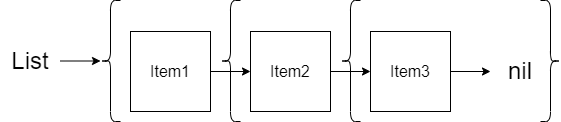
\includegraphics{images/ThreeItemCustomList.drawio.png}

The first item in each tuple represents the value in the list and the second item in the tuple represents the remainder of the list. This is very similar to the \([First|Rest]\) format we often write where \(First\) represents the first value in the list and the \(Rest\) represents the remainder of the list.

For simplicity, we will define a push and pop function which will only affect the front of our list.

\begin{formulabox}
\(struct ~ ~ list ~ ~ \lbrace a:First, list:Rest \rbrace.\)

\end{formulabox}

\(\nonumber\)

\begin{formulabox}
\(spec ~ ~ push :: a ~ ~ list \rightarrow list.\)

\(de\mathit{f} ~ ~ push :: Value ~ ~ List \rightarrow \lbrace Value, List \rbrace.\)

\end{formulabox}

\(\nonumber\)

\begin{formulabox}
\(spec ~ ~ pop :: list \rightarrow list.\)

\(de\mathit{f} ~ ~ pop :: nil \rightarrow nil\)

\(de\mathit{f} ~ ~ pop :: \lbrace First, Rest \rbrace \rightarrow Rest.\)

\end{formulabox}

\(\nonumber\)

Implementing this code we have the following:

\begin{Shaded}
\begin{Highlighting}[]
\FunctionTok{push(}\VariableTok{List}\FunctionTok{,} \VariableTok{Value}\FunctionTok{)} \OperatorTok{{-}\textgreater{}} \FunctionTok{\{}\VariableTok{Value}\FunctionTok{,} \VariableTok{List}\FunctionTok{\}.}

\FunctionTok{pop(}\CharTok{nil}\FunctionTok{)} \OperatorTok{{-}\textgreater{}} \CharTok{nil}\FunctionTok{;}
\FunctionTok{pop(\{}\VariableTok{\_First}\FunctionTok{,} \VariableTok{Rest}\FunctionTok{\})} \OperatorTok{{-}\textgreater{}} \VariableTok{Rest}\FunctionTok{.}
\end{Highlighting}
\end{Shaded}

If we wanted to calculate the length function, we would need to visit every item in our list to count. To avoid this, we can store the length as meta-data using a Monad. We will define our list Monad type to be: \texttt{\{List,\ Length\}}. Using this type, our example lists now look like this:

\begin{itemize}
\tightlist
\item
  Empty List: \texttt{\{nil,\ 0\}}
\item
  One Item List: \texttt{\{\{Item1,\ nil\},\ 1\}}
\item
  Two Item List: \texttt{\{\{Item1,\ \{Item2,\ nil\}\},\ 2\}}
\item
  Three Item List: \texttt{\{\{Item1,\ \{Item2,\ \{Item3,\ nil\}\}\},\ 3\}}
\end{itemize}

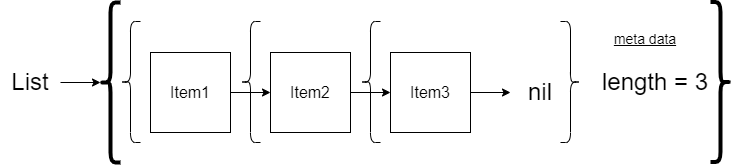
\includegraphics{images/ThreeItemCustomListMonad.drawio.png}

Recall that Monad functions don't take the Monad type as an input but they should return the Monad type. That will mean that when we call our \texttt{push} and \texttt{pop} functions, the length must be stripped off. How does the \texttt{push} and \texttt{pop} know what to set the length to in the result? Remember that the \texttt{bind} function is responsible for managing the meta data. We will have the \texttt{push} and \texttt{pop} return a delta length. For \texttt{push}, the delta length will be positive 1 and for \texttt{pop}, the delta length will be negative 1. We will have the \texttt{bind} manage the length meta-data.

In our specifications and definitions below, we will modify the \texttt{push} and \texttt{pop} to use the Monad type and also include the type constructor (in this case we will use a more interesting name like \texttt{create} instead of \texttt{unit}) for creating an empty list (length of 0) and the binding function. Since we will want the ability to see the list and length independent of the Monad type, we will provide some simple helper functions (\texttt{value} and \texttt{len}) for these as well.

The bind will be more complex because it will need to handle both \texttt{push} and \texttt{pop} functions which have different arity. The \([a]\) (called \texttt{Optional\_Parameters} in the definition) contains the variable number of parameters to pass to \texttt{push} and \texttt{pop}. We will use a traditional Erlang list data structure to store these parameters.

\begin{formulabox}
\(struct ~ ~ list ~ ~ \lbrace a:First, list:Rest \rbrace.\)

\(struct ~ ~ m\_list ~ ~ \lbrace list:List, integer:Length \rbrace.\)

\end{formulabox}

\(\nonumber\)

\begin{formulabox}
\(spec ~ ~ push :: a ~ ~ list \rightarrow m\_list.\)

\(de\mathit{f} ~ ~ push :: Value ~ ~ List \rightarrow \lbrace \lbrace Value, List \rbrace, 1\rbrace.\)

\end{formulabox}

\(\nonumber\)

\begin{formulabox}
\(spec ~ ~ pop :: list \rightarrow m\_list.\)

\(de\mathit{f} ~ ~ pop :: nil \rightarrow (create);\)

\(de\mathit{f} ~ ~ pop :: \lbrace First, Rest \rbrace \rightarrow \lbrace Rest, -1 \rbrace.\)

\end{formulabox}

\(\nonumber\)

\begin{formulabox}
\(spec ~ ~ create :: ~ ~ \rightarrow m\_list.\)

\(de\mathit{f} ~ ~ create :: \rightarrow \lbrace nil, 0 \rbrace.\)

\end{formulabox}

\(\nonumber\)

\begin{formulabox}
\(spec ~ ~ \lambda_{bind} :: list \rightarrow m\_list.\)

\(spec ~ ~ bind :: m\_list ~ ~ \lambda_{bind} ~ ~ [a] \rightarrow m\_list.\)

\(de\mathit{f} ~ ~ bind :: \lbrace List, Length \rbrace ~ ~ \lambda_{bind} ~ ~ Optional\_Parameters \rightarrow\)

\(\quad \quad \lbrace New\_List, Delta\_Length \rbrace = (\lambda_{bind} ~ ~ Optional\_Parameters ++ List),\)

\(\quad \quad \lbrace New\_List, Length + Delta\_Length \rbrace.\)

\end{formulabox}

\(\nonumber\)

\begin{formulabox}
\(spec ~ ~ value :: m\_list \rightarrow list.\)

\(de\mathit{f} ~ ~ value :: \lbrace List, Length \rbrace \rightarrow List.\)

\(spec ~ ~ len :: m\_list \rightarrow integer.\)

\(de\mathit{f} ~ ~ len :: \lbrace List, Length \rbrace \rightarrow Length.\)

\end{formulabox}

\(\nonumber\)

When implemented, you will need to use the \texttt{apply} function in Erlang to handle passing the \texttt{List} and \texttt{Optional\_Parameters} to the \(\lambda_{bind}\) function. If \texttt{push} is used, then the \texttt{Optional\_Parameters} will be a one element list containing the value to push. If \texttt{pop} is used, the \texttt{Optional\_Parameters} will be an empty list. Some of these functions are implemented below and some are left as an exercise.

\begin{Shaded}
\begin{Highlighting}[]
\FunctionTok{push(}\VariableTok{Value}\FunctionTok{,} \VariableTok{List}\FunctionTok{)} \OperatorTok{{-}\textgreater{}} \FunctionTok{\{\{}\VariableTok{Value}\FunctionTok{,} \VariableTok{List}\FunctionTok{\},}\DecValTok{1}\FunctionTok{\}.}

\CommentTok{\% pop is left as an exercise}
   
\FunctionTok{create()} \OperatorTok{{-}\textgreater{}} \FunctionTok{\{}\CharTok{nil}\FunctionTok{,} \DecValTok{0}\FunctionTok{\}.}

\FunctionTok{bind(\{}\VariableTok{List}\FunctionTok{,} \VariableTok{Length}\FunctionTok{\},} \VariableTok{Function}\FunctionTok{,} \VariableTok{Optional\_Parameters}\FunctionTok{)} \OperatorTok{{-}\textgreater{}} 
    \VariableTok{LEFT} \VariableTok{FOR} \VariableTok{AN} \VariableTok{EXERCISE}

\FunctionTok{len(\{}\VariableTok{\_List}\FunctionTok{,} \VariableTok{Length}\FunctionTok{\})} \OperatorTok{{-}\textgreater{}} \VariableTok{Length}\FunctionTok{.}
\FunctionTok{value(\{}\VariableTok{List}\FunctionTok{,} \VariableTok{\_Length}\FunctionTok{\})} \OperatorTok{{-}\textgreater{}} \VariableTok{List}\FunctionTok{.}
\end{Highlighting}
\end{Shaded}

For the length get updated, we have to use the bind function as shown in the test code below.

\begin{Shaded}
\begin{Highlighting}[]
\VariableTok{L1} \OperatorTok{=} \FunctionTok{create(),}
\VariableTok{L2} \OperatorTok{=} \FunctionTok{bind(}\VariableTok{L1}\FunctionTok{,} \KeywordTok{fun} \CharTok{push}\OperatorTok{/}\DecValTok{2}\FunctionTok{,} \FunctionTok{[}\DecValTok{2}\FunctionTok{]),}
\VariableTok{L3} \OperatorTok{=} \FunctionTok{bind(}\VariableTok{L2}\FunctionTok{,} \KeywordTok{fun} \CharTok{push}\OperatorTok{/}\DecValTok{2}\FunctionTok{,} \FunctionTok{[}\DecValTok{4}\FunctionTok{]),}
\VariableTok{L4} \OperatorTok{=} \FunctionTok{bind(}\VariableTok{L3}\FunctionTok{,} \KeywordTok{fun} \CharTok{push}\OperatorTok{/}\DecValTok{2}\FunctionTok{,} \FunctionTok{[}\DecValTok{6}\FunctionTok{]),}
\VariableTok{L5} \OperatorTok{=} \FunctionTok{bind(}\VariableTok{L4}\FunctionTok{,} \KeywordTok{fun} \CharTok{pop}\OperatorTok{/}\DecValTok{1}\FunctionTok{,} \FunctionTok{[]),}
\end{Highlighting}
\end{Shaded}

\begin{problembox}

\textbf{Problem Set 3}

\begin{enumerate}
\def\labelenumi{\arabic{enumi}.}
\item
  Implement the \texttt{pop} and \texttt{bind} function with the list Monad type. Use the code in the template to test. Note that the \texttt{apply} function is available in Erlang which will call a function and pass a variable list of arguments to the function. Use the code in the template to test.
\item
  Sometimes a function uses more than one Monad type. Since its possible for the \texttt{pop} to fail in the case of an empty list, it might be a good to use the \texttt{Maybe} monad type so we can return \texttt{\{fail\}} in that case. In the case of the \texttt{push}, we don't have any reason to return \texttt{\{fail\}}. However, to support the \texttt{bind}, we will be consistent and return the \texttt{Maybe} monad type. The \texttt{bind} needs to handle the case where one of our functions returns \texttt{\{fail\}}. When this happens, an empty list should be created and returned back (which is what \texttt{pop} currently does). We need to write three new functions: \texttt{push2}, \texttt{pop2}, and \texttt{bind2} that support \texttt{Maybe}. The \texttt{push2} function is already written for you. Use the specifications below and the tests provided in the starting code. The \texttt{bind2} function will likely need to use the \texttt{case\ of} block to determine what to do based on the result of running the \(\lambda_{bind2}\) function.
\end{enumerate}

\begin{formulabox}
\(struct ~ ~ maybe\_m\_list\)

\(\quad \quad \lbrace atom(ok), m\_list:Value \rbrace ~ ~ or\)

\(\quad \quad \lbrace atom(fail) \rbrace.\)

\(spec ~ ~ push2 :: a ~ ~ list \rightarrow maybe\_m\_list.\)

\(spec ~ ~ pop2 :: list \rightarrow maybe\_m\_list.\)

\(spec ~ ~ \lambda_{bind2} :: list \rightarrow maybe\_m\_list.\)

\(spec ~ ~ bind2 :: m\_list ~ ~ \lambda_{bind2} ~ ~ [a] \rightarrow m\_list.\)

\end{formulabox}

\end{problembox}

\(\nonumber\)
\(\nonumber\)
\href{http://creativecommons.org/licenses/by/4.0/}{
\includegraphics{images/cc-88x31.png}}

\hypertarget{streams-and-lazy-evaluation}{%
\chapter{Streams and Lazy Evaluation}\label{streams-and-lazy-evaluation}}

In this lesson we will learn about the Stream Design Pattern. Streams are things that provide you values when you need them. They are an example of the unfold functor pattern. This ``lazy'' approach can actually save you a lot of time and memory when you only need something one at a time.

\hypertarget{streams}{%
\section{Streams}\label{streams}}

A stream provides information to us one item at a time whenever we need it. This implies that when writing a stream, we need to consider two things:

\begin{itemize}
\tightlist
\item
  Provide the user a function to call when they are ready to get the next thing.
\item
  The function that we provide must be aware of what the previous thing was so it can give the next thing.
\end{itemize}

Let's look at both of these needs separately. If we wanted to provide the user with the ability to add 1 to a number at any time, we could write a function that return a function to be called later.

\begin{formulabox}
\(spec ~ ~ lazy\_incr\_once :: integer \rightarrow (\lambda :: \rightarrow integer).\)

\(de\mathit{f} ~ ~ lazy\_incr\_once :: Value \rightarrow (\lambda :: \rightarrow Value + 1).\)

\end{formulabox}

\(\nonumber\)

\begin{Shaded}
\begin{Highlighting}[]
\FunctionTok{lazy\_incr\_once(}\VariableTok{X}\FunctionTok{)} \OperatorTok{{-}\textgreater{}} \KeywordTok{fun}\FunctionTok{()} \OperatorTok{{-}\textgreater{}} \VariableTok{X} \OperatorTok{+} \DecValTok{1} \KeywordTok{end}\FunctionTok{.}

\FunctionTok{test()} \OperatorTok{{-}\textgreater{}}
    \VariableTok{L} \OperatorTok{=} \FunctionTok{lazy\_incr\_once(}\DecValTok{4}\FunctionTok{),}
    \DecValTok{5} \OperatorTok{=} \VariableTok{L}\FunctionTok{(),}
    \DecValTok{5} \OperatorTok{=} \VariableTok{L}\FunctionTok{(),}
    \CharTok{ok}\FunctionTok{.}
\end{Highlighting}
\end{Shaded}

In the code above, we are running the function that was returned when we called \texttt{lazy\_incr\_once}. Combine this concept with the desire to have the function return something based on the previous result. In the \texttt{lazy\_incr} function, we will return two things: the next value and the next function to call. Notice that we are defining a custom data type called \texttt{iterator} which will contain both of these things. Our ultimate goal by the next lesson is to define this as a Monad.

\begin{formulabox}
\(struct ~ ~ iterator ~ ~ \lbrace a, \lambda_{stream} \rbrace.\)

\(spec ~ ~ \lambda_{stream} :: \rightarrow iterator.\)

\(spec ~ ~ lazy\_incr :: integer \rightarrow \lambda_{stream}.\)

\(de\mathit{f} ~ ~ lazy\_incr :: Value \rightarrow (\lambda_{stream} :: \rightarrow \lbrace (Value + 1), (lazy\_incr ~ ~ (Value + 1)) \rbrace).\)

\end{formulabox}

\(\nonumber\)

\begin{Shaded}
\begin{Highlighting}[]
\FunctionTok{lazy\_incr(}\VariableTok{Value}\FunctionTok{)} \OperatorTok{{-}\textgreater{}} \KeywordTok{fun}\FunctionTok{()} \OperatorTok{{-}\textgreater{}} \FunctionTok{\{}\VariableTok{Value} \OperatorTok{+} \DecValTok{1}\FunctionTok{,} \FunctionTok{lazy\_incr(}\VariableTok{Value}\OperatorTok{+}\DecValTok{1}\FunctionTok{)\}} \KeywordTok{end}\FunctionTok{.}

\FunctionTok{test()} \OperatorTok{{-}\textgreater{}}
    \VariableTok{L} \OperatorTok{=} \FunctionTok{lazy\_incr(}\DecValTok{4}\FunctionTok{),}
    \FunctionTok{\{}\DecValTok{5}\FunctionTok{,} \VariableTok{L2}\FunctionTok{\}} \OperatorTok{=} \VariableTok{L}\FunctionTok{(),}
    \FunctionTok{\{}\DecValTok{6}\FunctionTok{,} \VariableTok{L3}\FunctionTok{\}} \OperatorTok{=} \VariableTok{L2}\FunctionTok{(),}
    \FunctionTok{\{}\DecValTok{7}\FunctionTok{,} \VariableTok{L4}\FunctionTok{\}} \OperatorTok{=} \VariableTok{L3}\FunctionTok{(),}
    \CharTok{ok}\FunctionTok{.}
\end{Highlighting}
\end{Shaded}

Another classic stream is the range function which will provide a sequence of numbers but only one at a time. In this function, we will assume that the sequence will from \texttt{Start} to \texttt{Stop}, inclusive and that \texttt{Start\ \textless{}=\ Stop}. Unlike the previous example, this iterator will need to stop. We will modify our new \texttt{fixed\_iterator} to have other possible values.

\begin{formulabox}
\(struct ~ ~ \mathit{f}ixed\_iterator\)

\(\quad \quad \lbrace a, \lambda_{stream} \rbrace ~ ~ or\)

\(\quad \quad \lbrace atom(unde\mathit{f}ined), atom(done) \rbrace.\)

\(spec ~ ~ \lambda_{stream} :: \rightarrow \mathit{f}ixed\_iterator.\)

\(spec ~ ~ range :: integer ~ ~ integer \rightarrow \lambda_{stream}.\)

\(de\mathit{f} ~ ~ range :: Start ~ ~ Stop \rightarrow (\lambda_{stream} :: \rightarrow \lbrace Start, (range ~ ~ (Start+1), Stop) \rbrace )\)

\(\quad \quad \text{when} ~ ~ Start \leq Stop;\)

\(de\mathit{f} ~ ~ range :: Start ~ ~ Stop \rightarrow (\lambda_{stream} :: \rightarrow \lbrace undefined, done \rbrace).\)

\end{formulabox}

\(\nonumber\)

The erlang code is given below:

\begin{Shaded}
\begin{Highlighting}[]
\FunctionTok{range(}\VariableTok{Start}\FunctionTok{,} \VariableTok{Stop}\FunctionTok{)} \CharTok{when} \VariableTok{Start} \OperatorTok{=\textless{}} \VariableTok{Stop} \OperatorTok{{-}\textgreater{}}
    \KeywordTok{fun} \FunctionTok{()} \OperatorTok{{-}\textgreater{}} \FunctionTok{\{}\VariableTok{Start}\FunctionTok{,} \FunctionTok{range(}\VariableTok{Start}\OperatorTok{+}\DecValTok{1}\FunctionTok{,} \VariableTok{Stop}\FunctionTok{)\}} \KeywordTok{end}\FunctionTok{;}
\FunctionTok{range(}\VariableTok{\_Start}\FunctionTok{,} \VariableTok{\_Stop}\FunctionTok{)} \OperatorTok{{-}\textgreater{}}
    \KeywordTok{fun} \FunctionTok{()} \OperatorTok{{-}\textgreater{}} \FunctionTok{\{}\CharTok{undefined}\FunctionTok{,} \CharTok{done}\FunctionTok{\}} \KeywordTok{end}\FunctionTok{.}
\end{Highlighting}
\end{Shaded}

We can simplify the above code by moving the guards into the anonymous function as shown below:

\begin{Shaded}
\begin{Highlighting}[]
\FunctionTok{range(}\VariableTok{Start}\FunctionTok{,} \VariableTok{Stop}\FunctionTok{)} \OperatorTok{{-}\textgreater{}}
    \KeywordTok{fun} \FunctionTok{()} \CharTok{when} \VariableTok{Start} \OperatorTok{=\textless{}} \VariableTok{Stop} \OperatorTok{{-}\textgreater{}} \FunctionTok{\{}\VariableTok{Start}\FunctionTok{,} \FunctionTok{range(}\VariableTok{Start}\OperatorTok{+}\DecValTok{1}\FunctionTok{,} \VariableTok{Stop}\FunctionTok{)\};}
        \FunctionTok{()} \OperatorTok{{-}\textgreater{}} \FunctionTok{\{}\CharTok{undefined}\FunctionTok{,} \CharTok{done}\FunctionTok{\}} \KeywordTok{end}\FunctionTok{.}
\end{Highlighting}
\end{Shaded}

An example of the test code using the \texttt{range} function is given below. Notice that the value of \texttt{\{undefined,\ done\}} is returned when the stream is completed.

\begin{Shaded}
\begin{Highlighting}[]
\FunctionTok{test()} \OperatorTok{{-}\textgreater{}}
    \VariableTok{Stream1} \OperatorTok{=} \FunctionTok{range(}\DecValTok{1}\FunctionTok{,}\DecValTok{4}\FunctionTok{),}
    \FunctionTok{\{}\DecValTok{1}\FunctionTok{,} \VariableTok{Stream2}\FunctionTok{\}} \OperatorTok{=} \VariableTok{Stream1}\FunctionTok{(),}
    \FunctionTok{\{}\DecValTok{2}\FunctionTok{,} \VariableTok{Stream3}\FunctionTok{\}} \OperatorTok{=} \VariableTok{Stream2}\FunctionTok{(),}
    \FunctionTok{\{}\DecValTok{3}\FunctionTok{,} \VariableTok{Stream4}\FunctionTok{\}} \OperatorTok{=} \VariableTok{Stream3}\FunctionTok{(),}
    \FunctionTok{\{}\DecValTok{4}\FunctionTok{,} \VariableTok{Stream5}\FunctionTok{\}} \OperatorTok{=} \VariableTok{Stream4}\FunctionTok{(),}
    \FunctionTok{\{}\CharTok{undefined}\FunctionTok{,} \CharTok{done}\FunctionTok{\}} \OperatorTok{=} \VariableTok{Stream5}\FunctionTok{(),}
    \CharTok{ok}\FunctionTok{.}
\end{Highlighting}
\end{Shaded}

\begin{problembox}

\textbf{Problem Set 1}

You can find the template for the problem sets in this lesson here: \href{proves/prove07.erl}{prove07.erl}

\begin{enumerate}
\def\labelenumi{\arabic{enumi}.}
\tightlist
\item
  Modify the \texttt{range} function to take a third parameter called \texttt{step}. You should increase the sequence by the amount of \texttt{step}. If the \texttt{step} is negative, then create a decreasing sequence. If the \texttt{step} is 0, then the \texttt{done} state should occur immediately. Test code is provided to test your stream.
\item
  Create a new stream called \texttt{words} which will split text by spaces into sub-strings Each time the stream is called, it should return back the next string. For example, if the text was ``The cow jumped over the moon.'', then the stream would first return ``The'', then ``cow'', then ``jumped'', and so forth. Use the \texttt{fixed\_iterator} Monad type described above. You are provided a function called \texttt{first\_word} which returns a tuple in the format \texttt{\{Word,\ Rest\}} where \texttt{Word} is the first word and \texttt{Rest} is the remaining text (just like working with values in a list). Test code is provided to test your stream.
\end{enumerate}

\end{problembox}

\hypertarget{stream-monad-collection}{%
\section{Stream Monad \& Collection}\label{stream-monad-collection}}

In the previous section we created a \texttt{fixed\_iterator} Monad that the \texttt{range} function supported. To complete the Monad definition, we need a type constructor (or unit function) and a bind function. Since the type constructor will need to create a stream that hasn't started yet, we will modify our specification for the Monad Type we had earlier (the second condition in the struct is new):

\begin{formulabox}
\(struct ~ ~ \mathit{f}ixed\_iterator\)

\(\quad \quad \lbrace a, \lambda_{stream} \rbrace ~ ~ or\)

\(\quad \quad \lbrace atom(unde\mathit{f}ined), \lambda_{stream} \rbrace ~ ~ or\)

\(\quad \quad \lbrace atom(unde\mathit{f}ined), atom(done) \rbrace.\)

\(spec ~ ~ \lambda_{stream} :: \rightarrow \mathit{f}ixed\_iterator.\)

\end{formulabox}

\(\nonumber\)

The type constructor should be used to create the iterator the first time. We will call our type constructor \texttt{iter}. The \texttt{iter} will take as an input a \(\lambda_{stream}\) function (the function that is returned by our \texttt{range} function or any other stream). The \texttt{iter} will produce the \(\lbrace atom(unde\mathit{f}ined), \lambda_{next} \rbrace\). This is the state of our iterator before we actually start the iteration.

\begin{formulabox}
\(spec ~ ~ iter :: \lambda_{stream} \rightarrow \mathit{f}ixed\_iterator.\)

\(de\mathit{f} ~ ~ iter :: \lambda_{stream} \rightarrow \lbrace unde\mathit{f}ined, \lambda_{stream} \rbrace.\)

\end{formulabox}

\(\nonumber\)

The bind should allow us to take our \texttt{fixed\_iterator} (the Monad type returned by the \texttt{iter} function) and pass it to our stream function which will return an updated \texttt{fixed\_iterator}. Remember that our stream function is always regenerated and has no input parameters. The next function is re-created each time with the next value built-into the function. We will call our bind function \texttt{next} and it will be responsible for getting the next stream iteration. Unlike previous bind functions we have used, this bind will not take a function parameter because it is applied only to our \(\lambda_{stream}\).

\begin{formulabox}
\(spec ~ ~ next :: \mathit{f}ixed\_iterator \rightarrow \mathit{f}ixed\_iterator.\)

\(de\mathit{f} ~ ~ next :: \lbrace Value, done \rbrace \rightarrow \lbrace unde\mathit{f}ined, done \rbrace;\)

\(de\mathit{f} ~ ~ next :: \lbrace Value, \lambda_{stream} \rbrace \rightarrow (\lambda_{stream}).\)

\end{formulabox}

\(\nonumber\)

Using these specifications and definitions, we can complete the \texttt{fixed\_iterator} Monad along with helper functions (\texttt{value} and \texttt{lambda}) to access both parts of our Monad type.

\begin{Shaded}
\begin{Highlighting}[]
\FunctionTok{iter(}\VariableTok{Stream}\FunctionTok{)} \OperatorTok{{-}\textgreater{}} \FunctionTok{\{}\CharTok{undefined}\FunctionTok{,} \VariableTok{Stream}\FunctionTok{\}.}

\FunctionTok{next(\{}\VariableTok{\_Value}\FunctionTok{,}\CharTok{done}\FunctionTok{\})} \OperatorTok{{-}\textgreater{}} \FunctionTok{\{}\CharTok{undefined}\FunctionTok{,} \CharTok{done}\FunctionTok{\};}
\FunctionTok{next(\{}\VariableTok{\_Value}\FunctionTok{,}\VariableTok{Lambda}\FunctionTok{\})} \OperatorTok{{-}\textgreater{}} \VariableTok{Lambda}\FunctionTok{().}

\FunctionTok{value(\{}\VariableTok{Value}\FunctionTok{,}\VariableTok{\_Lambda}\FunctionTok{\})} \OperatorTok{{-}\textgreater{}} \VariableTok{Value}\FunctionTok{.}
\FunctionTok{lambda(\{}\VariableTok{\_Value}\FunctionTok{,}\VariableTok{Lambda}\FunctionTok{\})} \OperatorTok{{-}\textgreater{}} \VariableTok{Lambda}\FunctionTok{.}
\end{Highlighting}
\end{Shaded}

We can use our new functions and show that calling our bind function \texttt{next} will result in \texttt{undefined} if we complete our iterator.

\begin{Shaded}
\begin{Highlighting}[]
\VariableTok{Next1} \OperatorTok{=} \FunctionTok{next(iter(range(}\DecValTok{1}\FunctionTok{,}\DecValTok{4}\FunctionTok{))),}
\FunctionTok{io:format(}\StringTok{"\textasciitilde{}p\textasciitilde{}n"}\FunctionTok{,[value(}\VariableTok{Next1}\FunctionTok{)]),}  \CommentTok{\% Print 1}
\VariableTok{Next2} \OperatorTok{=} \FunctionTok{next(}\VariableTok{Next1}\FunctionTok{),}
\FunctionTok{io:format(}\StringTok{"\textasciitilde{}p\textasciitilde{}n"}\FunctionTok{,[value(}\VariableTok{Next3}\FunctionTok{)]),}  \CommentTok{\% Print 2}
\VariableTok{Next3} \OperatorTok{=} \FunctionTok{next(}\VariableTok{Next2}\FunctionTok{),}
\FunctionTok{io:format(}\StringTok{"\textasciitilde{}p\textasciitilde{}n"}\FunctionTok{,[value(}\VariableTok{Next3}\FunctionTok{)]),}  \CommentTok{\% Print 3}
\VariableTok{Next4} \OperatorTok{=} \FunctionTok{next(}\VariableTok{Next3}\FunctionTok{),}
\FunctionTok{io:format(}\StringTok{"\textasciitilde{}p\textasciitilde{}n"}\FunctionTok{,[value(}\VariableTok{Next4}\FunctionTok{)]),}  \CommentTok{\% Print 4}
\VariableTok{Next5} \OperatorTok{=} \FunctionTok{next(}\VariableTok{Next4}\FunctionTok{),}
\FunctionTok{io:format(}\StringTok{"\textasciitilde{}p\textasciitilde{}n"}\FunctionTok{,[value(}\VariableTok{Next5}\FunctionTok{)]),}  \CommentTok{\% Print undefined}
\VariableTok{Next6} \OperatorTok{=} \FunctionTok{next(}\VariableTok{Next5}\FunctionTok{),}
\FunctionTok{io:format(}\StringTok{"\textasciitilde{}p\textasciitilde{}n"}\FunctionTok{,[value(}\VariableTok{Next6}\FunctionTok{)]),}  \CommentTok{\% Print undefined}
\end{Highlighting}
\end{Shaded}

A common function that is implemented when lazy streams are supported is the \texttt{collect}. The \texttt{collect} function will undo the ``laziness'' of our data structure by iterating through the entire \(\lambda_{stream}\) and put all the results in order into a traditional list.

The specification for the \texttt{collect} is given below:

\begin{formulabox}
\(spec ~ ~ collect :: \lambda_{stream} \rightarrow [a].\)

\(spec ~ ~ collect :: \lambda_{stream} ~ ~ [a] \rightarrow [a].\)

\end{formulabox}

\(\nonumber\)

The second specification is intended to help build the list result recursively by calling the \texttt{next} function until the iterator is completed. The definition for the first specification for \texttt{collect/1}is given below. Notice that the function will call \texttt{iter} to convert the \(\lambda_{stream}\) into a \texttt{fixed\_iterator} prior to doing the recursion to generate the list of values.

\begin{formulabox}
\(de\mathit{f} ~ ~ collect :: Stream \rightarrow (collect (iter ~ ~ Stream) ~ ~ []).\)

\end{formulabox}

\(\nonumber\)

The erlang code for \texttt{collect/1} is given below:

\begin{Shaded}
\begin{Highlighting}[]
\FunctionTok{collect(}\VariableTok{Stream}\FunctionTok{)} \OperatorTok{{-}\textgreater{}} \FunctionTok{(}\CharTok{collect} \FunctionTok{(}\CharTok{iter}\NormalTok{ \textasciitilde{} \textasciitilde{} }\VariableTok{Stream}\FunctionTok{),} \FunctionTok{[]).}
\end{Highlighting}
\end{Shaded}

The implementation of the \texttt{collect/2} function is left for an exercise below.

\begin{problembox}

\textbf{Problem Set 2}

\begin{enumerate}
\def\labelenumi{\arabic{enumi}.}
\tightlist
\item
  Implement the \texttt{collect/2} function and test it with the code provided. When writing the function, you should reuse the \texttt{next} function iterate the stream, reuse the \texttt{value} function to get the value to put in the \texttt{Result} list, and reuse the \texttt{lambda} function to compare with \texttt{done}. Test code using the \texttt{collect} function with \texttt{range} and \texttt{words} is provided.
\end{enumerate}

\end{problembox}

\hypertarget{erlang-processes-streams}{%
\section{Erlang Processes \& Streams}\label{erlang-processes-streams}}

Another common problem solved with streams is a unique ID generator. We could write the same code above to obtain a function that will return the next available number (i.e.~prev number + 1). However, if we had multiple software components that needed to use the same unique ID generator, then we need a slightly different approach.

Erlang supports a scalable process system that allows for safe concurrent operations. This process system can be used locally with our software or it can be used along with networking code to support communication between different machines.

The diagram below shows how a client/server process architecture can be setup in Erlang. We will assume in our discussion that both the client and the server are running locally on our same machine.

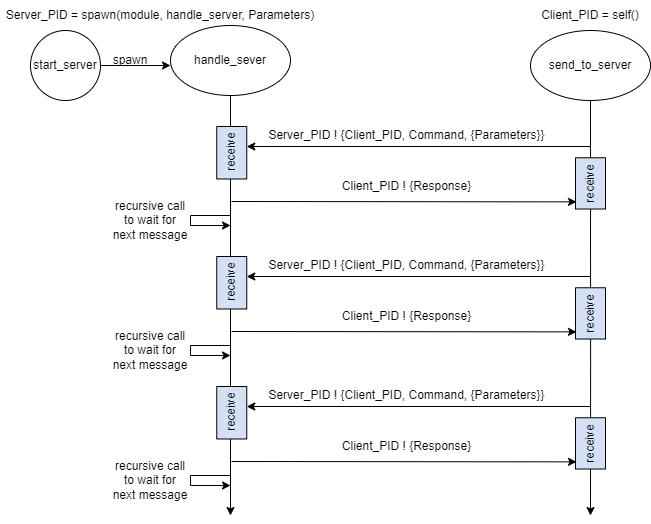
\includegraphics{images/client_server_erlang.drawio.png}

In the diagram above, we have a process that is started (or spawned) by \texttt{start\_server} and handles messages received by \texttt{handle\_server}. The client uses the server process ID (PID) to send messages to the server and then waits for a response. All messages sent to the server are formatted as follows:

\begin{formulabox}
\(\lbrace Client\_PID, Command, \lbrace Parameters \rbrace \rbrace\)

\end{formulabox}

\(\nonumber\)

Response back to the client are formatted as follows:

\begin{formulabox}
\(\lbrace Response \rbrace\)

\end{formulabox}

\(\nonumber\)

This simple server has only two commands:
* echo - Send the text back to the client
* add - Add the two numbers and send back the answer to the client.

The server can handle only one request at a time. After the server handles the request, the \texttt{handle\_server} function is called again to handle the next request. This ability to handle only one thing at a time will help us create the unique ID server later on. Let's first look at the Erlang code needed:

\begin{Shaded}
\begin{Highlighting}[]
\FunctionTok{handle\_server()} \OperatorTok{{-}\textgreater{}}
    \KeywordTok{receive}
        \FunctionTok{\{}\VariableTok{Client\_PID}\FunctionTok{,} \CharTok{echo}\FunctionTok{,} \FunctionTok{\{}\VariableTok{Text}\FunctionTok{\}\}} \OperatorTok{{-}\textgreater{}} \VariableTok{Client\_PID} \OperatorTok{!} \FunctionTok{\{}\VariableTok{Text}\FunctionTok{\};}
        \FunctionTok{\{}\VariableTok{Client\_PID}\FunctionTok{,} \CharTok{add}\FunctionTok{,} \FunctionTok{\{}\VariableTok{X}\FunctionTok{,} \VariableTok{Y}\FunctionTok{\}\}} \OperatorTok{{-}\textgreater{}} \VariableTok{Client\_PID} \OperatorTok{!} \FunctionTok{\{}\VariableTok{X}\OperatorTok{+}\VariableTok{Y}\FunctionTok{\}}
    \KeywordTok{end}\FunctionTok{,}
    \FunctionTok{handle\_server().}

\FunctionTok{start\_server()} \OperatorTok{{-}\textgreater{}}
    \FunctionTok{spawn(}\CharTok{prove07}\FunctionTok{,} \CharTok{handle\_server}\FunctionTok{,} \FunctionTok{[]).}
 
\FunctionTok{send\_to\_server(}\VariableTok{Server\_PID}\FunctionTok{,} \VariableTok{Command}\FunctionTok{,} \VariableTok{Params}\FunctionTok{)} \OperatorTok{{-}\textgreater{}}
    \VariableTok{Server\_PID} \OperatorTok{!} \FunctionTok{\{self(),} \VariableTok{Command}\FunctionTok{,} \VariableTok{Params}\FunctionTok{\},}
    \KeywordTok{receive}
        \FunctionTok{\{}\VariableTok{Response}\FunctionTok{\}} \OperatorTok{{-}\textgreater{}} \VariableTok{Response}
    \KeywordTok{end}\FunctionTok{.}
\end{Highlighting}
\end{Shaded}

The \texttt{start\_server} function will spawn a new process. When spawning a new process, the handler function is specified along with its module name and a list of any parameters. In this simple example, there are no parameters. Note that you have to export the \texttt{handle\_server} function for the \texttt{spawn} function to work properly.

The \texttt{handle\_server} function uses the \texttt{receive} command to receive a message from a client. When one is received and matches one of the patterns in the \texttt{receive} command block, then a response is sent back. In Erlang, a message is sent using the syntax: \texttt{PID\ !\ Message}. We use the Client PID that we received to send the response back. The call to \texttt{handle\_server} recursively at the end will allow the server to response to the next client.

The \texttt{send\_to\_server} function is a utility function to help us send a message to server and receive the response. When sending messages to the server, the Erlang function \texttt{self()} is called to obtain the client PID to send to the server. A test example is shown below:

\begin{Shaded}
\begin{Highlighting}[]
\NormalTok{2\textgreater{} Server\_PID = prove07:start\_server().}
\NormalTok{\textless{}0.85.0\textgreater{}}
\NormalTok{3\textgreater{} prove07:send\_to\_server(Server\_PID, echo, \{"Hello"\}).}
\NormalTok{"Hello"}
\NormalTok{4\textgreater{} prove07:send\_to\_server(Server\_PID, add, \{13, 8\}).    }
\NormalTok{21}
\NormalTok{5\textgreater{}}
\end{Highlighting}
\end{Shaded}

If we wanted to create a unique ID server following this same format, we can modify our handler function to take a parameter that keeps track of the current ID. Remember that each call to the handler function is guaranteed to handle only one client at a time. Similar to the concept of the stream functions being created with the next value in the stream, our handler will create the next value to be used.

Here is the code for our new \texttt{start\_id\_server} and \texttt{handle\_id\_server}. Notice that the \texttt{handle\_id\_server} now has an input parameter and it is initialized in the spawn function within \texttt{start\_id\_server}. For the \texttt{export}, notice that we specify the arity: \texttt{handle\_id\_server/1}.

\begin{Shaded}
\begin{Highlighting}[]
\KeywordTok{{-}export}\FunctionTok{([}\CharTok{handle\_id\_server}\OperatorTok{/}\DecValTok{1}\FunctionTok{]).}

\FunctionTok{handle\_id\_server(}\VariableTok{Curr\_ID}\FunctionTok{)} \OperatorTok{{-}\textgreater{}}
    \KeywordTok{receive}
        \FunctionTok{\{}\VariableTok{Client\_PID}\FunctionTok{,} \CharTok{id}\FunctionTok{,} \FunctionTok{\{\}\}} \OperatorTok{{-}\textgreater{}} \VariableTok{Client\_PID} \OperatorTok{!} \FunctionTok{\{}\VariableTok{Curr\_ID}\FunctionTok{\}}
    \KeywordTok{end}\FunctionTok{,}
    \FunctionTok{handle\_id\_server(}\VariableTok{Curr\_ID} \OperatorTok{+} \DecValTok{1}\FunctionTok{).}

\FunctionTok{start\_id\_server()} \OperatorTok{{-}\textgreater{}}
    \FunctionTok{spawn(}\CharTok{prove07}\FunctionTok{,} \CharTok{handle\_id\_server}\FunctionTok{,} \FunctionTok{[}\DecValTok{0}\FunctionTok{]).}
\end{Highlighting}
\end{Shaded}

When the \texttt{handle\_id\_server} is called recursively to handle the request from the next client, the \texttt{Unique\_ID} is incremented by 1.

Reusing the same \texttt{send\_to\_server} function, we can generate new unique ID's as follows starting with 0.

\begin{Shaded}
\begin{Highlighting}[]
\NormalTok{5\textgreater{} ID\_Server\_PID = prove07:start\_id\_server(). }
\NormalTok{\textless{}0.89.0\textgreater{}}
\NormalTok{6\textgreater{} prove07:send\_to\_server(ID\_Server\_PID, id, \{\}).       }
\NormalTok{0}
\NormalTok{7\textgreater{} prove07:send\_to\_server(ID\_Server\_PID, id, \{\}).}
\NormalTok{1}
\NormalTok{8\textgreater{} prove07:send\_to\_server(ID\_Server\_PID, id, \{\}).}
\NormalTok{2}
\NormalTok{9\textgreater{} prove07:send\_to\_server(ID\_Server\_PID, id, \{\}).}
\NormalTok{3}
\NormalTok{10\textgreater{} prove07:send\_to\_server(ID\_Server\_PID, id, \{\}).}
\NormalTok{4}
\NormalTok{11\textgreater{} prove07:send\_to\_server(ID\_Server\_PID, id, \{\}).}
\NormalTok{5}
\NormalTok{12\textgreater{} }
\end{Highlighting}
\end{Shaded}

\begin{problembox}

\textbf{Problem Set 3}

\begin{enumerate}
\def\labelenumi{\arabic{enumi}.}
\tightlist
\item
  Modify the \texttt{handle\_server} function to support an \texttt{avg} command that will average a variable collection of numbers. For example, if the parameters field is \texttt{\{10,20,30,40\}} then 25 will be returned back to the client. You can use the Erlang \texttt{lists:sum} and \texttt{length} functions.
\item
  Create a server based on the Unique ID server but with functions called \texttt{handle\_running\_avg\_server} (remember that this one needs to be exported) and \texttt{start\_running\_avg\_server} that maintains a running average of numbers submitted. There should be three commands:

  \begin{itemize}
  \tightlist
  \item
    add - Adds a number to the running average and returns the current average
  \item
    remove - Removes a number from the running average and returns the current average
  \item
    display - Returns the current average
  \end{itemize}

  When implementing the running average server, you should save the current sum and current number of numbers in your server. You should not store the list of numbers. Test code is provided for you.
\end{enumerate}

\end{problembox}

\(\nonumber\)
\(\nonumber\)
\href{http://creativecommons.org/licenses/by/4.0/}{
\includegraphics{images/cc-88x31.png}}

\hypertarget{trees}{%
\chapter{Trees}\label{trees}}

In this lesson we will learn about our second data structure called the Binary Search Tree. When we learned about persistence we learned about the list as it is implemented in Erlang. When we learned about monads, we introduced a new version of the list which was created using our own custom tuples. The Binary Search Tree will use this same custom approach.

\hypertarget{binary-search-tree}{%
\section{Binary Search Tree}\label{binary-search-tree}}

A binary search tree is a tree that stores smaller values to the left and larger values to the right. Each node in the tree in defined by 3 fields: value, link to the left sub-tree, and link to the right sub-tree.

The tree is useful because we can quickly search for values by asking ourselves, ``is the value we are looking for larger or smaller (or maybe we found it) than the one in the current node of the tree?'' This is like guessing a number between 1 and 100 and always guessing 50 first. Searching in the tree will ideally exclude half of the values with each comparison. We will explore this ``ideal'' performance in the next part of the lesson.

Persistence is a curious thing to consider visually with the tree. In the diagram below, we show the creation of a tree with one node valued 10 called \(T_1\) .

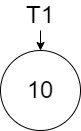
\includegraphics{images/bst_1.drawio.png}

When we add a new node with value 7 (in this case something that will go left of the root node), we must persist \(T_1\). Since the left link in the root node must change, then we need a new node to create \(T_2\).

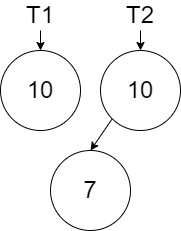
\includegraphics{images/bst_2.drawio.png}

If we now add a node with value 15 to the right of the root node, we are only affecting the right link. The new node we created in the previous step can be reused in creating \(T_3\).

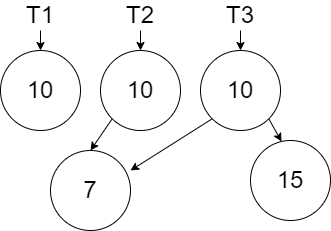
\includegraphics{images/bst_3.drawio.png}

In the next diagram we show the creation of \(T_4\) by adding the new node with value 13.

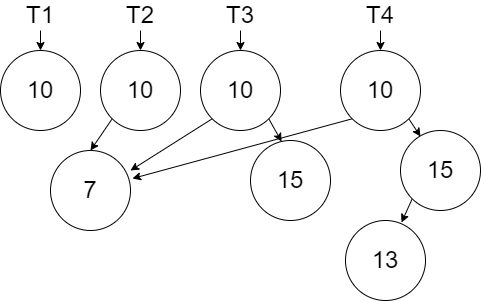
\includegraphics{images/bst_4.drawio.png}

In the next diagram we show the creation of \(T_5\) by adding the new node with value 9.

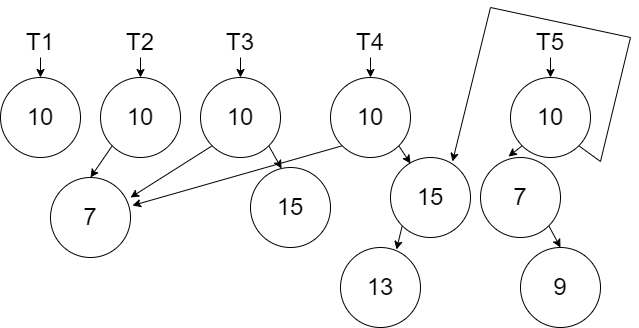
\includegraphics{images/bst_5.drawio.png}

Finally, we show the creation of \(T_6\) by adding the new new node 5.

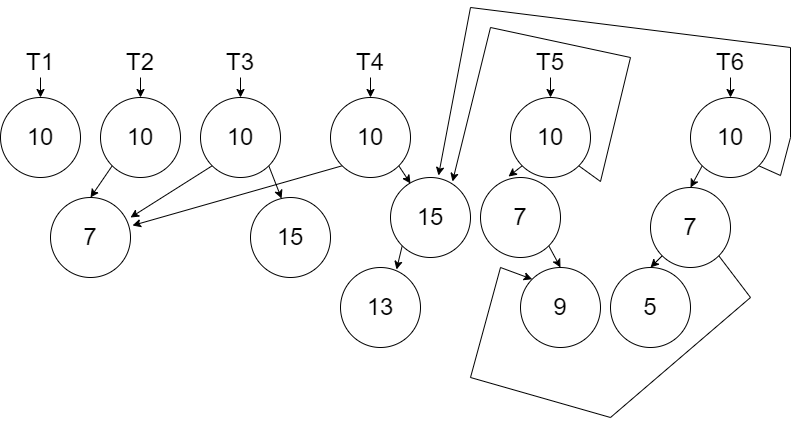
\includegraphics{images/bst_6.drawio.png}

The software will discard older versions of the Tree when they are not needed anymore. However, the persistence we use in the data structure is important to satisfy the immutability rules.

Notice that the there is always a path through the tree that we have to re-create from the root node down to the node that we added. When we reuse a node in the tree, we will reuse both the node and all the nodes it is connected too. We will not have to have use recursion when we reuse a node.

Let's begin with the structure of the node:

\begin{formulabox}
\(struct ~ ~ node ~ ~ \lbrace a:Value, node:\mathit{Left}, node:Right \rbrace.\)

\end{formulabox}

\(\nonumber\)

We will implement two functions in our binary search tree. The \texttt{add} function will add a value to the tree and the \texttt{contains} function will search the tree for a value and return a true or false. When we add to a tree or we search in a tree, we will do so recursively through nodes beginning with the root node. When we add to a tree, the result will be an updated root node (or an updated sub-tree root node as we recursively create our new tree).

\begin{formulabox}
\(spec ~ ~ add :: a ~ ~ node \rightarrow node.\)

\(spec ~ ~ contains :: a ~ ~ node \rightarrow boolean.\)

\end{formulabox}

\(\nonumber\)

In our specification, we are assuming that \(a\) represents a type that can be compared with boolean operators.

There are 4 scenarios when adding a new item to a tree:
* Empty Tree - Create a new root \texttt{node}. We will define an empty tree as \texttt{nil}.
* Value to add is less than the current node value - Create a new \texttt{node} reusing the right link. The left link is created by recursively calling \texttt{add} on the left sub-tree.
* Value to add is greater than the current node value - Create a new \texttt{node} reusing the left link. The right link is created by recursively calling \texttt{add} on the right sub-tree.
* Value to add is equal to the current node value - In our tree, we will require all values to be unique. In this case, we get to reuse the entire node including both left and right links. The tree can be implemented differently by allowing duplicates perhaps stored to the right.

The definition for \texttt{add} is given below. The implementation for both \texttt{add} and \texttt{contains} will be left for an exercise.

\begin{formulabox}
\(\mathit{def} ~ ~ add :: New\_Value ~ ~ nil \rightarrow \lbrace New\_Value, nil, nil \rbrace;\)

\(\mathit{def} ~ ~ add :: New\_Value ~ ~ \lbrace Value, Left, Right \rbrace \rightarrow \lbrace Value, (add ~ ~ New\_Value ~ ~ Left), Right \rbrace ~ ~ \text{when} ~ ~ New\_Value < Value;\)

\(\mathit{def} ~ ~ add :: New\_Value ~ ~ \lbrace Value, Left, Right \rbrace \rightarrow \lbrace Value, Left, (add ~ ~ New\_Value ~ ~ Right) \rbrace ~ ~ \text{when} ~ ~ New\_Value > Value;\)

\(\mathit{def} ~ ~ add :: New\_Value ~ ~ Node \rightarrow Node.\)

\end{formulabox}

\(\nonumber\)

\begin{problembox}

\textbf{Problem Set 1}

You can find the template for the problem sets in this lesson here: \href{proves/prove08.erl}{prove08.erl}

\begin{enumerate}
\def\labelenumi{\arabic{enumi}.}
\tightlist
\item
  Implement the \texttt{add} function per the specification and definition above. Use the test code provided.
\item
  Implement the \texttt{contains} function per the specification above. Use the test code provided.
\end{enumerate}

\end{problembox}

\hypertarget{balanced-red-black-tree}{%
\section{Balanced Red-Black Tree}\label{balanced-red-black-tree}}

Since a binary search tree orders left and right of node relative to the values, traversing the tree (either to insert or find) can provide an O(log n) performance. However, this can only be achieved if the tree is balanced. If we added the numbers 1, 2, 3, 4, 5, 6, 7 in order to a tree, they would also be add to the right. Searching for a number in the tree would be the same as searching a list which is O(n)

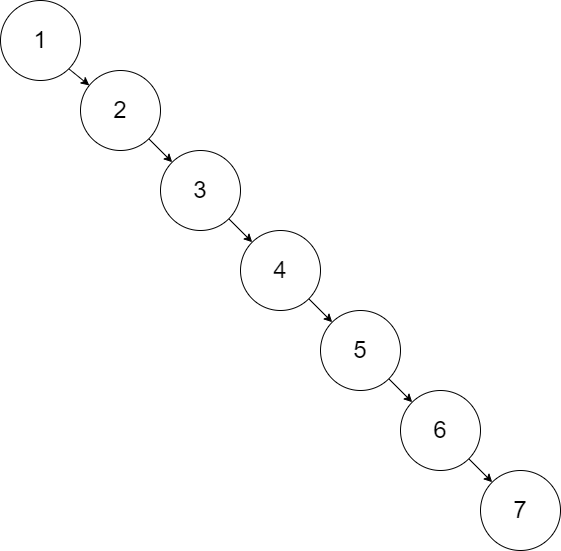
\includegraphics{images/unbalanced_tree.drawio.png}

However, if the numbers were added 4, 2, 6, 1, 3, 5, 7 then we would get a tree that allows for the maximum exclusion of values every time we go left or right.

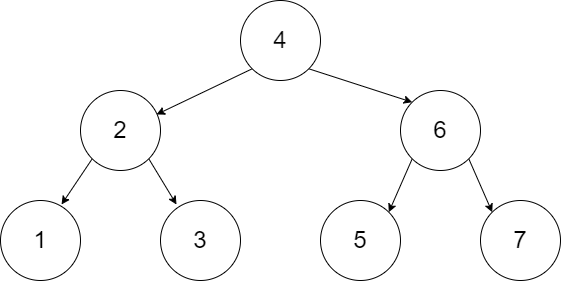
\includegraphics{images/balanced_tree.drawio.png}

Since we can't rely on the order of the data, there are other strategies and algorithms that can be used. A common one is the Red Back Tree (RBT). The RBT uses a set of rules to determine if part of a tree is unbalanced. If something is unbalanced, a modification is made to balance the tree. In other words, after the creation of any node in the \texttt{add} function, we will potentially perform a \texttt{balance} function.

The rules for an RBT are as follows:

\begin{enumerate}
\def\labelenumi{\arabic{enumi}.}
\tightlist
\item
  Every node is either red or black - In our algorithm we will choose to start all nodes out red.
\item
  The root is always black - In our algorithm we will choose to change the root node to black after the inserting and all balancing is completed.
\item
  No two adjacent nodes are red.
\item
  Every path from a node to a leaf has the same number of black nodes.
\end{enumerate}

In our algorithm we will enforce rules and 3 and 4 with our balancing function.

To support these rules, the structure of the node must change to include the color of the node:

\begin{formulabox}
\(struct ~ ~ node\)

\(\quad \quad \lbrace atom(red), a:Value, node:\mathit{Left}, node:Right \rbrace ~ ~ or\)

\(\quad \quad \lbrace atom(black), a:Value, node:\mathit{Left}, node:Right \rbrace.\)

\end{formulabox}

\(\nonumber\)

We will use the function names \texttt{add\_rbt} and \texttt{contains\_rbt} so they are unique from the traditional binary search tree. These \texttt{contains\_rbt} is the same as \texttt{contains} as the color is only important for adding and therefore is unused in the \texttt{contains\_rbt}.

The \texttt{add\_rbt} function is very similar to the \texttt{add} with the following distinctions:
* When we create a new node we color it red
* When we create a new node that reuses one link and recursively adds the node on the other link, we need to call a \texttt{balance} function (discussed later) on the new node we created.
* When we are done adding the node, we need to change the root node to be black. This will necessitate a helper function so that we have \texttt{add\_rbt} and \texttt{add\_rbt\_} both.

The specification and definition for the \texttt{add\_rbt} is shown below:

\begin{formulabox}
\(spec ~ ~ add\_rbt :: a ~ ~ node \rightarrow node.\)

\(spec ~ ~ add\_rbt\_ :: a ~ ~ node \rightarrow node.\)

\(\mathit{def} ~ ~ add\_rbt :: New\_Value ~ ~ Tree \rightarrow\)

\(\quad \quad New\_Root = (add\_rbt\_ ~ ~ New\_Value ~ ~ Tree),\)

\(\quad \quad \lbrace black, New\_Root.Value, New\_Root.\mathit{Left}, New\_Root.Right \rbrace.\)

\(\mathit{def} ~ ~ add\_rbt\_ :: New\_Value ~ ~ nil \rightarrow \lbrace red, New\_Value, nil, nil \rbrace;\)

\(\mathit{def} ~ ~ add\_rbt\_ :: New\_Value ~ ~ \lbrace Color, Value, \mathit{Left}, Right \rbrace \rightarrow\)

\(\quad \quad (balance ~ ~ \lbrace Color, Value, (add\_rbt\_ ~ ~ New\_Value ~ ~ \mathit{Left}), Right \rbrace) ~ ~\)

\(\quad \quad \text{when} ~ ~ New\_Value < Value;\)

\(\mathit{def} ~ ~ add\_rbt\_ :: New\_Value ~ ~ \lbrace Color, Value, \mathit{Left}, Right \rbrace \rightarrow\)

\(\quad \quad (balance ~ ~ \lbrace Color, Value, Left, (add\_rbt\_ ~ ~ New\_Value ~ ~ \mathit{Right}) \rbrace) ~ ~\)

\(\quad \quad \text{when} ~ ~ New\_Value > Value;\)

\(\mathit{def} ~ ~ add\_rbt\_ :: New\_Value ~ ~ Node \rightarrow Node.\)

\end{formulabox}

\(\nonumber\)

The \texttt{balance} function that is being performed is based on pattern matching defined by an algorithm written by Chris Okasaki (reference Purely Functional Data Structures). In his algorithm, there are four unbalanced scenarios that need to be balanced. These adjustments are made when the \texttt{add\_rbt\_} function is returning from all the recursive calls back up to the new root. The diagram below shows the four scenarios.

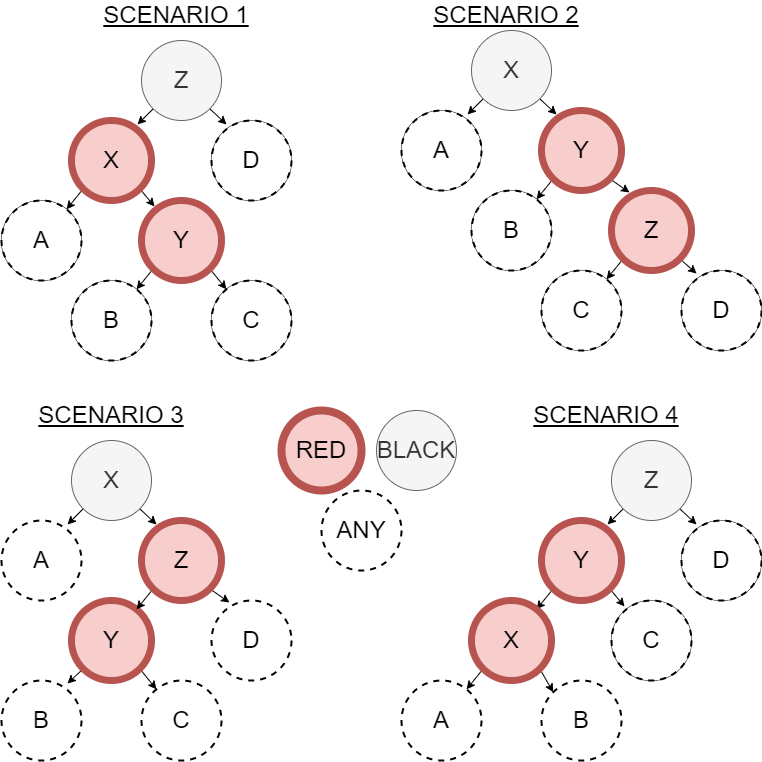
\includegraphics{images/rbt_balance.drawio.png}

The selection of variables in these diagrams was purposeful to suggest that \(X < Y < Z\). We need code to look for each of these four scenarios. If we have any of these four, then the solution is the same shown below.

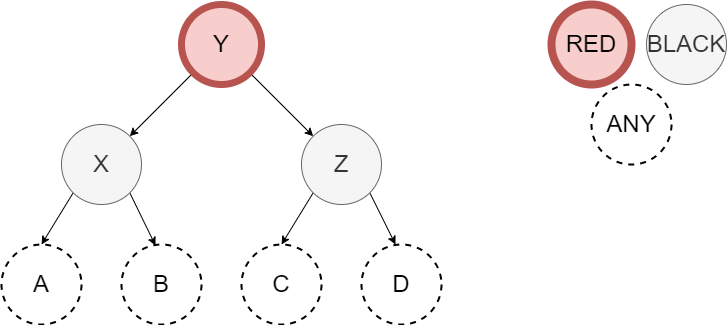
\includegraphics{images/rbt_balance_result.drawio.png}

The specification for our balance is simple as it converts a potentially unbalanced node into a balanced node:

\begin{formulabox}
\(spec ~ ~ balance :: node \rightarrow node.\)

\end{formulabox}

\(\nonumber\)

The definition for this function has 5 clauses (one for each scenario plus one in case none of them match. The first clause below corresponds to scenario 1. The next three scenarios are left for an exercise. The default clause is also given below.

\begin{formulabox}
\(\mathit{def} ~ ~ balance :: \lbrace black, Z, \lbrace red, X, A, \lbrace red, Y, B, C, \rbrace \rbrace, D \rbrace) \rightarrow\)

\(\quad \quad \lbrace red, Y, \lbrace black, X, A, B \rbrace, \lbrace black, Z, C, D \rbrace \rbrace;\)

\(\mathit{def} ~ ~ balance :: \text{Scenario 2 left for an exercise};\)

\(\mathit{def} ~ ~ balance :: \text{Scenario 3 left for an exercise};\)

\(\mathit{def} ~ ~ balance :: \text{Scenario 4 left for an exercise};\)

\(\mathit{def} ~ ~ balance :: Node \rightarrow Node.\)

\end{formulabox}

\(\nonumber\)

The Erlang code for the definitions provided above is given below. The remaining code is left for an exercise.

\begin{Shaded}
\begin{Highlighting}[]
\FunctionTok{balance(\{}\CharTok{black}\FunctionTok{,}\VariableTok{Z}\FunctionTok{,\{}\CharTok{red}\FunctionTok{,}\VariableTok{X}\FunctionTok{,}\VariableTok{A}\FunctionTok{,\{}\CharTok{red}\FunctionTok{,}\VariableTok{Y}\FunctionTok{,}\VariableTok{B}\FunctionTok{,}\VariableTok{C}\FunctionTok{\}\},}\VariableTok{D}\FunctionTok{\})} \OperatorTok{{-}\textgreater{}} \FunctionTok{\{}\CharTok{red}\FunctionTok{,}\VariableTok{Y}\FunctionTok{,\{}\CharTok{black}\FunctionTok{,}\VariableTok{X}\FunctionTok{,}\VariableTok{A}\FunctionTok{,}\VariableTok{B}\FunctionTok{\},\{}\CharTok{black}\FunctionTok{,}\VariableTok{Z}\FunctionTok{,}\VariableTok{C}\FunctionTok{,}\VariableTok{D}\FunctionTok{\}\};}
\CommentTok{\% Scenarios 2, 3, and 4 are left for an exercise}
\FunctionTok{balance(}\VariableTok{Node}\FunctionTok{)} \OperatorTok{{-}\textgreater{}} \VariableTok{Node}\FunctionTok{.}
\end{Highlighting}
\end{Shaded}

\begin{problembox}
\textbf{Problem Set 2}

\begin{enumerate}
\def\labelenumi{\arabic{enumi}.}
\tightlist
\item
  Complete the add functionality for the RBT. The \texttt{add\_rbt} function is written for you and you need to write the \texttt{add\_rbt\_} as described in the specification and definition above. Implement the \texttt{add\_rbt\_} function per the specification and definition above. You will also need to finish implementing the \texttt{balance} function for cases 2, 3, and 4 per the diagrams above. Use the test code provided.
\item
  Implement the \texttt{contains\_rbt} function per the specification below. Note that while color is used in the RBT, the color is left unused by the \texttt{contains\_rbt} function. Use the test code provided.
\end{enumerate}

\begin{formulabox}
\(spec ~ ~ contains\_rbt :: a ~ ~ node \rightarrow boolean.\)

\end{formulabox}

\(\nonumber\)

\end{problembox}

\hypertarget{performance}{%
\section{Performance}\label{performance}}

The binary search tree from Part 1 has performance of O(log n) if its balanced but as it becomes unbalanced, it becomes O(n). The RBT from Part 2 has performance of O(log n) because it maintains the balanced state. Even though there is more work needed to balance, it is offset by ability to find the spot for new nodes because its balanced.

To compare the performance of both approaches for a tree with 10,000 nodes in the problem set below, we will use the \texttt{eprof} library in Erlang. This library will report the number of times a function runs and the execution time of those functions. As with tools like these, there is an overhead cost for running \texttt{eprof} but it will not prevent us from making observations.

The following utility functions can be put around code to display performance results.

\begin{Shaded}
\begin{Highlighting}[]
\FunctionTok{start\_perf()} \OperatorTok{{-}\textgreater{}}
    \FunctionTok{eprof:start\_profiling([self()]).}

\FunctionTok{stop\_perf(}\VariableTok{Title}\FunctionTok{)} \OperatorTok{{-}\textgreater{}}
    \FunctionTok{io:format(}\StringTok{"Perf (\textasciitilde{}p): \textasciitilde{}n"}\FunctionTok{,[}\VariableTok{Title}\FunctionTok{]),}
    \FunctionTok{eprof:stop\_profiling(),}
    \FunctionTok{eprof:analyze(}\CharTok{total}\FunctionTok{).}
\end{Highlighting}
\end{Shaded}

If we wanted to compare the cost of adding to the front of a list and the cost of adding to the end of list, we would create a single \texttt{foldl} to perform those operations using a sequence of numbers from 1 to 10,000.

\begin{Shaded}
\begin{Highlighting}[]
\CommentTok{\% Code to test}
\FunctionTok{prepend(}\VariableTok{Value}\FunctionTok{,} \VariableTok{List}\FunctionTok{)} \OperatorTok{{-}\textgreater{}} \FunctionTok{[}\VariableTok{Value}\FunctionTok{|}\VariableTok{List}\FunctionTok{].}

\FunctionTok{append(}\VariableTok{Value}\FunctionTok{,[])} \OperatorTok{{-}\textgreater{}} \FunctionTok{[}\VariableTok{Value}\FunctionTok{];}
\FunctionTok{append(}\VariableTok{Value}\FunctionTok{,[}\VariableTok{First}\FunctionTok{|}\VariableTok{Rest}\FunctionTok{])} \OperatorTok{{-}\textgreater{}} \FunctionTok{[}\VariableTok{First}\FunctionTok{|append(}\VariableTok{Value}\FunctionTok{,}\VariableTok{Rest}\FunctionTok{)].}

\FunctionTok{timing\_test()} \OperatorTok{{-}\textgreater{}}
    \VariableTok{List} \OperatorTok{=} \FunctionTok{lists:seq(}\DecValTok{1}\FunctionTok{,}\DecValTok{10000}\FunctionTok{),}
    
    \FunctionTok{start\_perf(),}
    \FunctionTok{lists:foldl(}\KeywordTok{fun} \CharTok{prepend}\OperatorTok{/}\DecValTok{2}\FunctionTok{,} \FunctionTok{[],} \VariableTok{List}\FunctionTok{),}
    \FunctionTok{stop\_perf(}\StringTok{"prepend"}\FunctionTok{),}

    \FunctionTok{start\_perf(),}
    \FunctionTok{lists:foldl(}\KeywordTok{fun} \CharTok{append}\OperatorTok{/}\DecValTok{2}\FunctionTok{,} \FunctionTok{[],} \VariableTok{List}\FunctionTok{),}
    \FunctionTok{stop\_perf(}\StringTok{"append"}\FunctionTok{),}

    \CharTok{ok}\FunctionTok{.}
\end{Highlighting}
\end{Shaded}

The code will take several seconds to run. The output of \texttt{eprof} will include your functions and several others. Sample output (results will vary on different computers) of \texttt{eprof} for this code including only the functions we are testing is given below:

\begin{Shaded}
\begin{Highlighting}[]
\NormalTok{Perf ("prepend"):}
\NormalTok{FUNCTION                          CALLS        \%  TIME  [uS / CALLS]}
\NormalTok{{-}{-}{-}{-}{-}{-}{-}{-}                          {-}{-}{-}{-}{-}  {-}{-}{-}{-}{-}{-}{-}  {-}{-}{-}{-}  [{-}{-}{-}{-}{-}{-}{-}{-}{-}{-}]}
\NormalTok{prove08:prepend/2                 10000    22.91  1126  [      0.11]}
\NormalTok{{-}{-}{-}{-}{-}{-}{-}{-}{-}{-}{-}{-}{-}{-}{-}{-}{-}{-}{-}{-}{-}{-}{-}{-}{-}{-}{-}{-}{-}{-}{-}{-}  {-}{-}{-}{-}{-}  {-}{-}{-}{-}{-}{-}{-}  {-}{-}{-}{-}  [{-}{-}{-}{-}{-}{-}{-}{-}{-}{-}]}
\NormalTok{Total:                            32524  100.00\%  4914  [      0.15]}

\NormalTok{Perf ("append"): }
\NormalTok{FUNCTION                             CALLS        \%     TIME  [uS / CALLS]}
\NormalTok{{-}{-}{-}{-}{-}{-}{-}{-}                             {-}{-}{-}{-}{-}  {-}{-}{-}{-}{-}{-}{-}     {-}{-}{-}{-}  [{-}{-}{-}{-}{-}{-}{-}{-}{-}{-}]}
\NormalTok{prove08:append/2                  50005000    99.94  9867673  [      0.20]}
\NormalTok{{-}{-}{-}{-}{-}{-}{-}{-}{-}{-}{-}{-}{-}{-}{-}{-}{-}{-}{-}{-}{-}{-}{-}{-}{-}{-}{-}{-}{-}{-}{-}{-}  {-}{-}{-}{-}{-}{-}{-}{-}  {-}{-}{-}{-}{-}{-}{-}  {-}{-}{-}{-}{-}{-}{-}  [{-}{-}{-}{-}{-}{-}{-}{-}{-}{-}]}
\NormalTok{Total:                            50027524  100.00\%  9873713  [      0.20]}
\end{Highlighting}
\end{Shaded}

We can see that the \texttt{prepend} was much faster taking about 1 millisecond versus \texttt{append} taking almost 10 seconds. The cost of each call wasn't too much different. The \texttt{append} was plagued by all the recursive calls to add the item to the end of the list. We can see the O(n\textsuperscript{2}) behavior of \texttt{append} when add \texttt{n} items.

\begin{problembox}

\textbf{Problem Set 3}

\begin{enumerate}
\def\labelenumi{\arabic{enumi}.}
\tightlist
\item
  Compare the performance of the Binary Search Tree (\texttt{add} and \texttt{contains}) and the Red Black Tree (\texttt{add\_rbt} and \texttt{contains\_rbt}). Use the \texttt{start\_perf} and \texttt{stop\_perf} functions to add up the total time using these functions (remember that \texttt{add\_rbt} uses \texttt{add\_rbt\_} and \texttt{balance} as well). Add the numbers 1 to 10,000 (the list is already provided to you in the test code) to both data structures in order using a \texttt{foldl}. This will result in the worst unbalanced tree using \texttt{add}. Do a search for the value 10,000 to force the largest search for both \texttt{contains} and \texttt{contains\_rbt}). Compare the performances for our 4 functions and explain what you found.
\end{enumerate}

\end{problembox}

\(\nonumber\)
\(\nonumber\)
\href{http://creativecommons.org/licenses/by/4.0/}{
\includegraphics{images/cc-88x31.png}}

\hypertarget{min-heaps}{%
\chapter{Min Heaps}\label{min-heaps}}

In this lesson we will learn about Min Heaps. The Min Heap has two components to it: a minimum value easily accessible at the root and a ``heap'' of everything else below it in the form of a tree. There is a strategy for that heap of values which we will explore in the material below.

\hypertarget{min-heap}{%
\section{Min Heap}\label{min-heap}}

The diagram below shows a Min Heap. More specifically its a ``Leftist'' Min Heap since in all cases we have favored putting items on the left thus keeping the right ``spine'' of the tree as short as possible (within the algorithm requirements which we will learn about shortly).

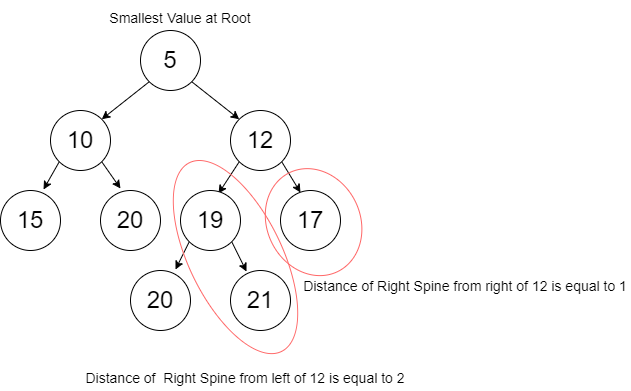
\includegraphics{images/heap_example.drawio.png}

When we look at this Min Heap, we see three characteristics:
1. The smallest value is in the root node
2. The values along each right spine (both from the root and from other nodes) are sorted.\\
3. For each node, the length of the right spine from the left and right links are such that the one on the left is greater than or equal to the one of the right. For example, if you look at node 12, the left side (node 19) has a distance of 2 on the right spine (following 19 and 21) and the right side (node 13) has a distance of 1 on the right spine (following only 13). We call this distance, the ``rank''.

If we want to add items to this Min Heap, we are going to add them in order along the right spine starting with the root node. When we insert in the node, we will need to work our way back up the tree and check to make sure we have not violated our need to have the left rank be greater than or equal to the right rank. If there is a problem, the solution is to just swap the left with the right.

Before we look at specifications, definitions, and code, we will first build a Min Heap by adding the following numbers in order (same values you will find in the test code for the problem set): 10, 15, 20, 5, 12, 17, 19, 20, 21, 13, 8, and 1. As you look at this list of numbers, note that we will have some interesting results at various times. For example, when add the 5 and the 1 we will be replacing the root node since the root node must contain the minimum value. Also, when we add 13, we will be replacing along the right spine from the root since the right spine from any node must be in order. In all of these operations, remember that we are persisting previous versions of the min heap.

The addition of our first node 10 is trivial since the min heap is empty. In each of these diagrams, we will show the rank on the upper right of the circle.

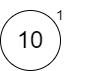
\includegraphics{images/heap1.drawio.png}

The addition of 15 will require us to compare it with 10 (the first only value on the right spine from the root). When we insert, we will always insert to the Right. When we get to the case that we are inserting in the middle of the spine, we will keep the left of our new node empty and the right of the new node will be the remainder of the spine unchanged.

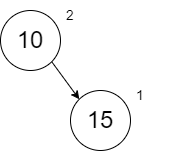
\includegraphics{images/heap2.drawio.png}

When we look at this min heap, notice that the rank on the right side is 1 and the left hand side is empty which implies a rank of 0. This means we need to swap left and right. The diagram below is correct.

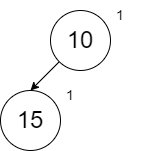
\includegraphics{images/heap3.drawio.png}

When we add 20, we have a spot and no swapping is needed.

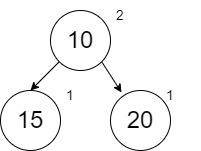
\includegraphics{images/heap4.drawio.png}

When we add 5, our first comparison shows that 5 should be before 20 on the right spine. When adding a new node to anywhere but the end of the spine, we will leave the left link empty and the right link will be the remainder of the spine unchanged. After doing this, we work our way back up (not too far in this case) to check ranks. We don't check the ranks of the spine that we left unchanged. The ranks at node 5 show that we need to swap.

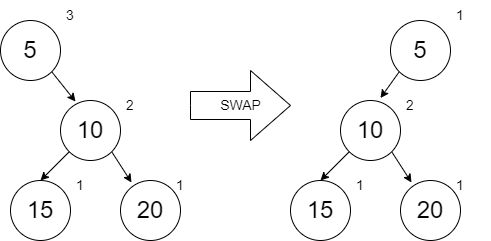
\includegraphics{images/heap5.drawio.png}

When we add 12, it can be done with no swapping.

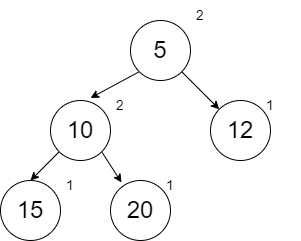
\includegraphics{images/heap6.drawio.png}

When we add 17, we start our comparisons with the node that we added (which is no issues because its at the end) and then work our way up the spine comparing ranks. At the 12, we see a need to swap.

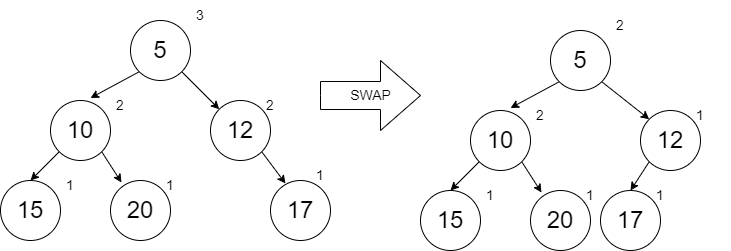
\includegraphics{images/heap7.drawio.png}

When we add the 19, it can be done with no swapping.

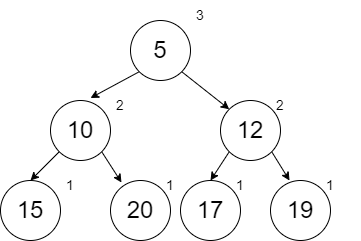
\includegraphics{images/heap8.drawio.png}

When we add the 20, it can also be done with no swapping. Notice that there was no problem adding this duplicate. If the duplicate was the root node already, we could choose to replace it with our new value and push the duplicate down (all depends on how we write our boolean comparison).

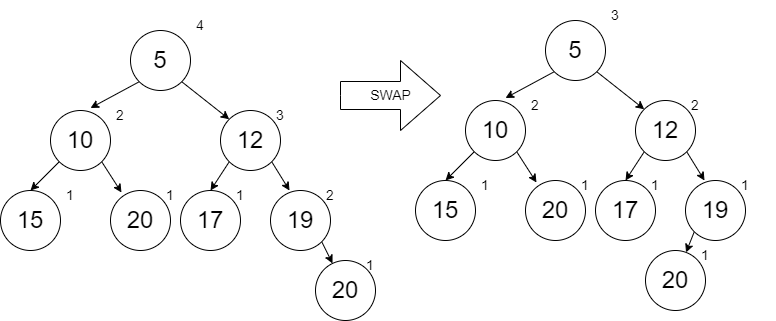
\includegraphics{images/heap9.drawio.png}

When we add the 21, we find that the node 12 has a need to swap.

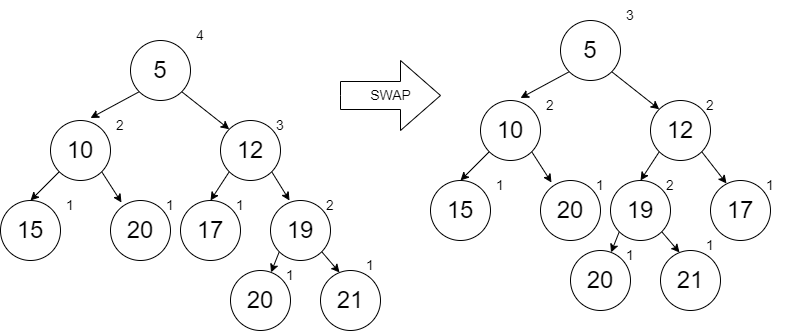
\includegraphics{images/heap10.drawio.png}

When we add the 13 (which occurs between 12 and 17), a swap occurs with node 13.

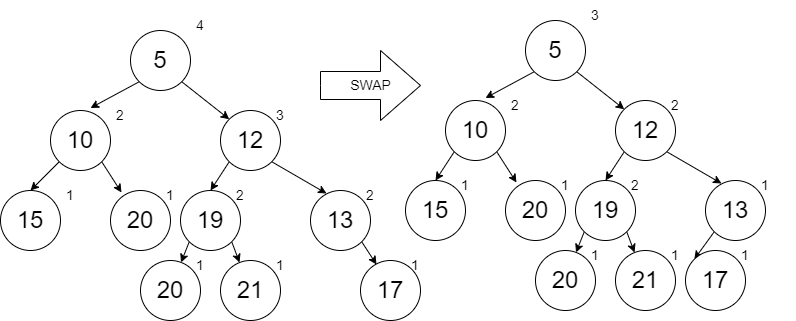
\includegraphics{images/heap11.drawio.png}

When we add the 8, we have to add it within the spine after the 5. When we do this, the rest of the spine is put to the right of our new node 8. Starting with node 8, we see the rank of node 12 is higher than the empty left side of 8. A swap is required. Notice as we do this that the right spine from the root is remaining minimized and sorted. This makes it faster to insert new items.

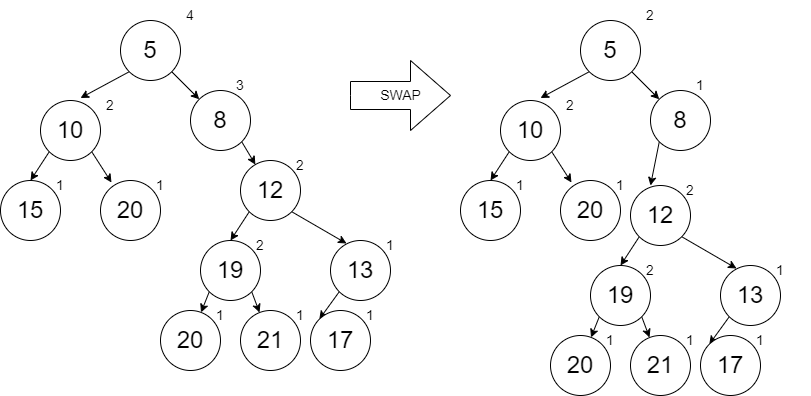
\includegraphics{images/heap12.drawio.png}

Finally, when we add the 1, it has to be added at the root, so the entire tree becomes the right link from the new 1 node. The ranks require us to swap and now we end of with a min heap that has nothing on the right side at all. This means inserting the next thing will be really fast and the minimum is easily accessible at the root still.

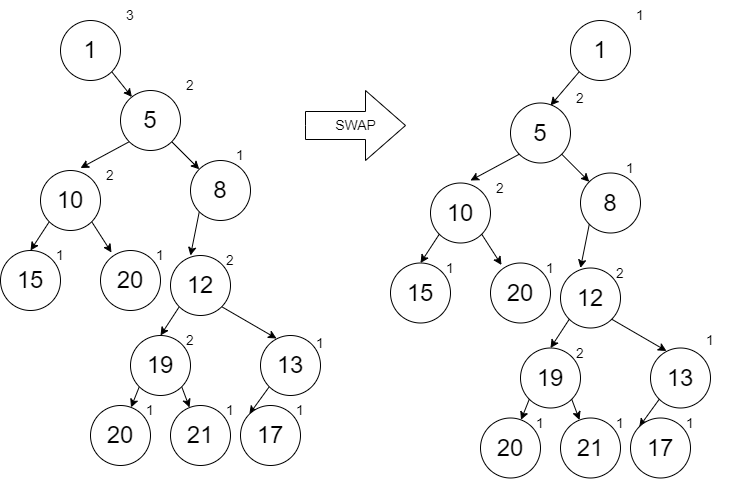
\includegraphics{images/heap13.drawio.png}

After reviewing this process, you should be able to envision the specification and design. We will be doing this in 2 steps. First, we will implement the inserting along the right spine but without swapping. The swapping will be done in the next section. We will define a structure that includes rank. We again are assuming that the data type \(a\) for the value is something that can be compared with boolean operators.

\begin{formulabox}
\(struct ~ ~ node ~ ~ \lbrace integer:Rank, a:Value, node:\mathit{Left}, node:Right \rbrace.\)

\(spec ~ ~ insert :: a ~ ~ node \rightarrow node.\)

\end{formulabox}

\(\nonumber\)

To support our definitions that we will discuss below, we have two helper functions (which will be more helpful as we explore this more). The \texttt{rank} function gives us a value of 0 when no node exists (\texttt{nil}). The \texttt{make} function will create the node with an updated rank value. Note that the distance along the right spine is always the rank of the right node plus one (representing the new node we are creating).

\begin{formulabox}
\(spec ~ ~ rank :: node \rightarrow integer.\)

\(spec ~ ~ make :: a ~ ~ node ~ ~ node \rightarrow node.\)

\(\mathit{def} ~ ~ rank :: nil \rightarrow 0;\)

\(\mathit{def} ~ ~ rank :: \lbrace Rank, Value, \mathit{Left}, Right \rbrace \rightarrow Rank.\)

\(\mathit{def} ~ ~ make :: Value ~ ~ \mathit{Left} ~ ~ Right \rightarrow \lbrace (rank ~ ~ Right) + 1, Value, \mathit{Left}, Right \rbrace.\)

\end{formulabox}

\(\nonumber\)

In the definition for \texttt{insert}, the first clause is for the case that we have reached the end of the spine (or the heap was empty to begin with). The second clause handles the case where we have found a place to insert along the spine. In this second case, we are keeping the entire remaining heap (\texttt{Node}) on the right of our new node. The third clause handles the case where we are still looking. In this last case, we are keeping the left link of the heap unchanged as we go.

\begin{formulabox}
\(\mathit{def} ~ ~ insert :: New\_Value ~ ~ nil \rightarrow (make ~ ~ New\_Value ~ ~ nil ~ ~ nil);\)

\(\mathit{def} ~ ~ insert :: New\_Value ~ ~ Node \rightarrow (make ~ ~ New\_Value ~ ~ nil ~ ~ Node)~ ~\)

\(\quad \quad \text{when} ~ ~ New\_Value \leq Node.Value;\)

\(\mathit{def} ~ ~ insert :: New\_Value ~ ~ Node \rightarrow (make ~ ~ Node.Value ~ ~ Node.\mathit{Left} ~ ~\)

\(\quad \quad (insert ~ ~ New\_Value ~ ~ Node.Right)).\)

\end{formulabox}

\(\nonumber\)

\begin{problembox}
\textbf{Problem Set 1}

You can find the template for the problem sets in this lesson here: \href{proves/prove09.erl}{prove09.erl}

\begin{enumerate}
\def\labelenumi{\arabic{enumi}.}
\tightlist
\item
  Implement the \texttt{insert} function per the specification and definition given above. The \texttt{rank} and \texttt{make} functions are written for you. Use the test code provided to test your function. Note that at this point, the algorithm has not done any swapping. That will be done in the next section below. When implementing this in Erlang, you may want to take advantage of some additional syntax. Up to this point, there are two ways you know to write the \texttt{insert} function with the \texttt{node} tuple:
\end{enumerate}

\begin{Shaded}
\begin{Highlighting}[]
\FunctionTok{insert(}\VariableTok{New\_Value}\FunctionTok{,} \VariableTok{Node}\FunctionTok{)} \OperatorTok{{-}\textgreater{}} \FunctionTok{...}
\CommentTok{\% or}
\FunctionTok{insert(}\VariableTok{New\_Value}\FunctionTok{,\{}\VariableTok{Rank}\FunctionTok{,} \VariableTok{Value}\FunctionTok{,} \VariableTok{Left}\FunctionTok{,} \VariableTok{Right}\FunctionTok{\})} \OperatorTok{{-}\textgreater{}} \FunctionTok{...}
\end{Highlighting}
\end{Shaded}

A third option combines both of these:

\begin{Shaded}
\begin{Highlighting}[]
\FunctionTok{insert(}\VariableTok{New\_Value}\FunctionTok{,} \VariableTok{Node}\OperatorTok{=}\FunctionTok{\{}\VariableTok{Rank}\FunctionTok{,} \VariableTok{Value}\FunctionTok{,} \VariableTok{Left}\FunctionTok{,} \VariableTok{Right}\FunctionTok{\})} \OperatorTok{{-}\textgreater{}} \FunctionTok{...}
\end{Highlighting}
\end{Shaded}

Using this third option, I can easily reference the whole \texttt{Node} or one its pieces by name. If the latter is done, you can also replace unused parameters with \texttt{\_} if desired.

\end{problembox}

\hypertarget{efficient-inserting-and-removal}{%
\section{Efficient Inserting and Removal}\label{efficient-inserting-and-removal}}

In the \texttt{insert} function we have created, no swapping has occurred. However, we have satisfied the first two rules that the minimum is a the root and the values in the right spines are all in order. Here is the result of our \texttt{insert} function using the values in the previous problem set:

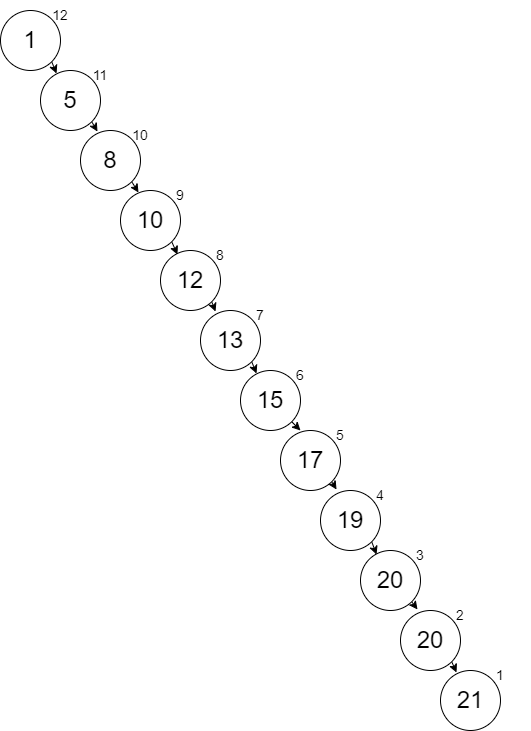
\includegraphics{images/heap_bad.drawio.png}

Notice that this looks like a list. The cost to find a place to insert a new node is O(n). If we do the swapping, we will minimize the length of the right spine and achieve O(log n).

To do the swapping, we will modify the definition of our make function. The first scenario below will not swap (\texttt{Left} is put on the left side, \texttt{Right} is put on the right side, and \texttt{Rank} is based on the \texttt{Right} rank) because Left Rank is larger or equal. The second scenario will swap because Left Rank is less. The second scenario is not shown below but is left for an exercise.

\begin{formulabox}
\(\mathit{def} ~ ~ make :: Value ~ ~ \mathit{Left} ~ ~ Right \rightarrow\)

\(\quad \quad Rank\_Left = (rank ~ ~ \mathit{Left}),\)

\(\quad \quad Rank\_Right = (rank ~ ~ Right),\)

\(\quad \quad \lbrace Rank\_Right + 1, Value, \mathit{Left}, Right \rbrace ~ ~ \text{when} ~ ~ Rank\_L \geq Rank\_R;\)

\end{formulabox}

\(\nonumber\)

The implementation of this updated \texttt{make} function will be left for an exercise below.

We will add many things to a min heap but the only thing we want to remove is the minimum value at the root. Obtaining this value is not difficult. However, removing from the heap and merging the left and right sides of the heap together is more complicated. Consider the following min heap (which is a smaller version of the previous example):

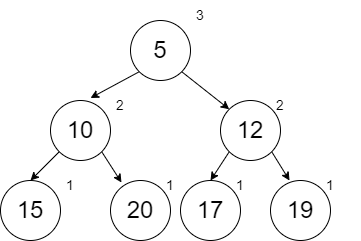
\includegraphics{images/heap_del1.drawio.png}

If we remove the root node 5, then we are left with two separate min heaps that need to be merged together. Here is the process:

\begin{enumerate}
\def\labelenumi{\arabic{enumi}.}
\tightlist
\item
  Follow the right spines of both min heaps recursively looking for the next largest value until you run out of ``spine'' on one of the heaps. The heap that you still have left becomes your new starting heap.
\item
  As you recursively return back up to the smaller values, insert the next smaller value one at a time (following the processes we used before including swapping as needed) into our new merged heap. When you insert the smaller values in, make sure that you include unchanged what was on their left.
\end{enumerate}

Following our process recursively down on the min heaps above, here is the order in which we went through to the largest value until one min heap was done. Notice that after the 19 was visited, the min heap on the right was done and so are starting min heap (from step 1 above) is just the node 20.

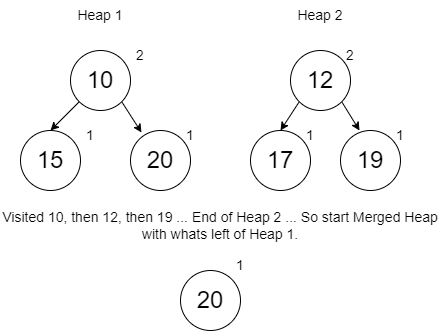
\includegraphics{images/heap_del2.drawio.png}

Working backwards, we merge in the 19 (which per our original process of inserting, it goes before the 20 and the 20 unchanged goes to the right) and get the following (after the required swapping to keep the min heap rules satisfied):

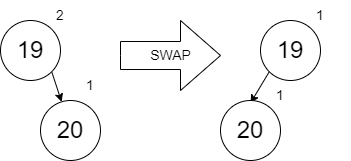
\includegraphics{images/heap_del3.drawio.png}

The next to merge in is the 12 (with the left node 17 unchanged):

\includegraphics{images/heap_del4.drawio.png}

The last to merge in is the 10 (with the left node 15 unchanged):

\includegraphics{images/heap_del5.drawio.png}

As expected, the new root is 10 which is new minimum value.

If we remove the 10, our second min heap to merge has only one node which is just like inserting a single value into the first min heap (which follows the same process of our two steps above).

\includegraphics{images/heap_del6.drawio.png}

Removing the 12:

\includegraphics{images/heap_del7.drawio.png}

Removing the 15:

\includegraphics{images/heap_del8.drawio.png}

With nothing left on the right hand side, the merging will become trivial as we remove more minimum values.

The specification for the merge is given below:

\begin{formulabox}
\(spec ~ ~ merge :: node ~ ~ node \rightarrow node.\)

\end{formulabox}

\(\nonumber\)

There are four scenarios for the definition. The first two handle the case of merging something with nothing. This is how we start with a heap after going through the complete right spine of one of the min heaps. The third scenario is if we find the next largest one on the right min heap. The fourth scenario is if we find the next largest one of the left min heap. In both of these last two scenarios, we keep going until we finish one of the spines and then we build the nodes up one at a time backwards using the \texttt{merge} function (which also takes care of our swapping).

\begin{formulabox}
\(\mathit{def} ~ ~ merge :: Heap1 ~ ~ nil \rightarrow Heap1;\)

\(\mathit{def} ~ ~ merge :: nil ~ ~ Heap2 \rightarrow Heap2;\)

\(\mathit{def} ~ ~ merge :: Heap1 ~ ~ Heap2 \rightarrow (make ~ ~ Heap1.Value, Heap1.Left,\)

\(\quad \quad (merge ~ ~ Heap1.Right, Heap2)) ~ ~ \text{when} ~ ~ Heap1.Value \leq Heap2.Value;\)

\(\mathit{def} ~ ~ merge :: Heap1 ~ ~ Heap2 \rightarrow (make ~ ~ Heap2.Value, Heap2.Left,\)

\(\quad \quad (merge ~ ~ Heap1, Heap2.Right));\)

\end{formulabox}

\(\nonumber\)

The \texttt{merge} function can now be used in a \texttt{remove\_min} function. The \texttt{remove\_min} function has the following specification:

\begin{formulabox}
\(spec ~ ~ remove\_min :: node \rightarrow node.\)

\end{formulabox}

\(\nonumber\)

The implementation of \texttt{merge} and \texttt{remove\_min} are left for exercises.

Since the \texttt{merge} function successfully handled merging a min heap with another min heap of size 1, we could reuse the \texttt{merge} function to simplify our \texttt{insert} function. We are merging our new node (created with \texttt{make}) with our existing min heap (\texttt{Node} - which could be nil).

\begin{Shaded}
\begin{Highlighting}[]
\FunctionTok{insert(}\VariableTok{New\_Value}\FunctionTok{,} \VariableTok{Node}\FunctionTok{)} \OperatorTok{{-}\textgreater{}} \FunctionTok{merge(make(}\VariableTok{New\_Value}\FunctionTok{,} \CharTok{nil}\FunctionTok{,} \CharTok{nil}\FunctionTok{),} \VariableTok{Node}\FunctionTok{).}
\end{Highlighting}
\end{Shaded}

\begin{problembox}

\textbf{Problem Set 2}

\begin{enumerate}
\def\labelenumi{\arabic{enumi}.}
\tightlist
\item
  Modify the existing \texttt{make} function to properly perform the swaps per the definition above (including the second scenario in the definition which was not provided to you). Use the test code provided to test your function.\\
\item
  Implement the \texttt{merge} function and the \texttt{remove\_min} function as described above. Use the test code provided to test your function. Once your code is working, you can modify your \texttt{insert} function to use the code provided above that uses \texttt{merge}.
\end{enumerate}

\end{problembox}

\hypertarget{priority-queue}{%
\section{Priority Queue}\label{priority-queue}}

A priority queue is a normal First In First Out (FIFO) queue except that a priority is added to each node placed in the queue. For our discussion, we will say that priority 1 is the highest priority and therefore should be processed first. The min heap is useful for a priority queue because the next item to dequeue is always quickly available at the root.

We want to modify our min heap so that it will work with any data \(a\) even if Erlang doesn't know how to compare with a boolean operator. The comparison (so long as we simplified our \texttt{insert} function already in the previous section) is only performed in the \texttt{merge} function. If we provide a function to our \texttt{merge} that handles the comparison, then we are unlimited to what we can put in our heap.

For a phone queue, we will define the following structure:

\begin{formulabox}
\(struct ~ ~ call ~ ~ \lbrace integer:Priority, string:Name \rbrace.\)

\end{formulabox}

\(\nonumber\)

In our \texttt{merge} function, we have been doing a \(\leq\) comparisons with the priority. Now we want to define a \(\leq\) comparison for \texttt{call} objects.

\begin{formulabox}
\(spec ~ ~ \lambda_{compare} :: call ~ ~ call \rightarrow boolean.\)

\end{formulabox}

\(\nonumber\)

If we are going to provide this \(\lambda_{compare}\) to our \texttt{merge} function, we are going to need to create a \texttt{merge/3}. Since \texttt{merge} is called by \texttt{insert} and \texttt{remove\_min}, we will need to create an \texttt{insert/3} and \texttt{remove\_min/2} as well to receive the \(\lambda_{compare}\).

\begin{formulabox}
\(spec ~ ~ insert :: a ~ ~ node ~ ~ \lambda_{compare} \rightarrow node.\)

\(spec ~ ~ remove\_min :: node ~ ~ \lambda_{compare} \rightarrow node.\)

\end{formulabox}

\(\nonumber\)

The implementation of \texttt{merge/3}, \texttt{insert/3}, and \texttt{remove\_min/2} along with the creation of a \(\lambda_{compare}\) to compare the priorities within two \texttt{call} tuples is left as an exercise below.

When we implement and test these functions, you should notice an unusual behavior when you have duplicate priorities. The order in which items are added to the min heap are not maintained when considering those items that have the same priorities. The Min Heap is not sort stable. The Min Heap will not guarantee the original order for duplicate priorities. Perhaps it could be useful to add a timestamp to our \texttt{call} record to keep track of who arrived first and then include that in our \(\lambda_{compare}\) function.

\begin{problembox}

\textbf{Problem Set 3}

\begin{enumerate}
\def\labelenumi{\arabic{enumi}.}
\tightlist
\item
  Implement the \texttt{merge/3}, \texttt{insert/3}, and \texttt{remove\_min/2} functions as described above. Modify the provided test code to set the variable \texttt{Calls\_Compare} equal to a your \(\lambda_{compare}\) which should compare two \texttt{call} tuples in the same way as the original \texttt{merge/2} compared two nodes with \(\leq\). For example, if \texttt{Calls\_Compare} was called on \texttt{\{"MST",\ 2,\ "Tim"\}} and \texttt{\{"PST",\ 1,\ "George"\}}, then the function would compare \(2 \leq 1\) which is \texttt{false}. Use the test code to test your code. Note that \texttt{get\_min} was implemented for you to support the test code.
\end{enumerate}

\end{problembox}

\(\nonumber\)
\(\nonumber\)
\href{http://creativecommons.org/licenses/by/4.0/}{\includegraphics{images/cc-88x31.png}}

\hypertarget{random-access-lists}{%
\chapter{Random Access Lists}\label{random-access-lists}}

The lists that we have used in this course have been linked lists. If we want to find something in the list, we have to search resulting in O(n) performance. We could use a binary search tree or a min heap to help us find things better but then we lose the order in which items were added. The name of dynamic arrays for which you can maintain order and have good lookup by index is done differently in functional languages when compared to the python list, the java ArrayList, or the C++ vector. A common solution is the Random Access List (RAL).

\hypertarget{binary-numbers-and-the-ral}{%
\section{Binary Numbers and the RAL}\label{binary-numbers-and-the-ral}}

In Erlang, there is not a way to quickly access a specific index in a list with O(1). In Part 3, you will explore the performance of the \texttt{nth} function that Erlang provides to do this. The difficulty is that we have to traverse through the entire list from beginning to the target index. To improve on this, we would like to find an O(log n) solution that maintains the order of the values. O(log n) makes us think about binary search trees. However, we need to store information in the trees that keeps the order the same. Binary Search Trees sacrifice order for performance.

To find a solution, we will consider a problem that at first does not seem related. Consider binary numbers (purposefully with leading zeros) going from 1 to 7: 001, 010, 011, 100, 101, 110, and 111. When we want to add 1 to our number, we will go from right to left and do one of the following:

\begin{itemize}
\tightlist
\item
  If we encounter a 0, we will replace it with a 1 and make no more changes.
\item
  If we encounter a 1, we will replace it with a 0 and consider these two steps again for the next number in the sequence. In this case we are mathematically carrying the 1 to the next item in the sequence.
\end{itemize}

If we try to do this in Erlang, we will be frustrated by the fact that we are going from right to left. Since it is more natural to go left (index 0) to right, we will flip our binary numbers around. When we read right to left, we call this little endian notation whereas when we read left to right, we call this big endian notation. To work better in Erlang, we will use the big endian notation

\begin{longtable}[]{@{}
  >{\raggedright\arraybackslash}p{(\columnwidth - 4\tabcolsep) * \real{0.3333}}
  >{\raggedright\arraybackslash}p{(\columnwidth - 4\tabcolsep) * \real{0.3333}}
  >{\raggedright\arraybackslash}p{(\columnwidth - 4\tabcolsep) * \real{0.3333}}@{}}
\toprule
\begin{minipage}[b]{\linewidth}\raggedright
Base 10 Value
\end{minipage} & \begin{minipage}[b]{\linewidth}\raggedright
Little Endian Notation (Right to Left)
\end{minipage} & \begin{minipage}[b]{\linewidth}\raggedright
Big Endian Notation (Left to Right)
\end{minipage} \\
\midrule
\endhead
1 & 001 & 100 \\
2 & 010 & 010 \\
3 & 011 & 110 \\
4 & 100 & 001 \\
5 & 101 & 101 \\
6 & 110 & 011 \\
7 & 111 & 111 \\
\bottomrule
\end{longtable}

Here is the specification and definition for incrementing a binary sequence (going left to right in big endian format) where the sequence starts at 1 and the sequence is stored in a list. Note that the definition follows the two rules for incrementing a binary sequence that we identified earlier. An empty list would represent the value of 0.

\begin{formulabox}
\(spec ~ ~ inc :: [integer] \rightarrow [integer].\)

\(de\mathit{f} ~ ~ inc :: [0|Rest] \rightarrow [1|Rest];\)

\(de\mathit{f} ~ ~ inc :: [1|Rest] \rightarrow [0|( inc ~ ~ Rest)];\)

\end{formulabox}

\(\nonumber\)

The erlang code is shown below:

\begin{Shaded}
\begin{Highlighting}[]
\FunctionTok{inc([])} \OperatorTok{{-}\textgreater{}} \FunctionTok{[}\DecValTok{1}\FunctionTok{];}
\FunctionTok{inc([}\DecValTok{0}\FunctionTok{|}\VariableTok{Rest}\FunctionTok{])} \OperatorTok{{-}\textgreater{}} \FunctionTok{[}\DecValTok{1}\FunctionTok{|}\VariableTok{Rest}\FunctionTok{];}
\FunctionTok{inc([}\DecValTok{1}\FunctionTok{|}\VariableTok{Rest}\FunctionTok{])} \OperatorTok{{-}\textgreater{}} \FunctionTok{[}\DecValTok{0}\FunctionTok{|inc(}\VariableTok{Rest}\FunctionTok{)].}

\FunctionTok{test()} \OperatorTok{{-}\textgreater{}}
    \FunctionTok{lists:foldl(}
        \KeywordTok{fun}\FunctionTok{(}\VariableTok{\_Value}\FunctionTok{,}\VariableTok{Acc}\FunctionTok{)} \OperatorTok{{-}\textgreater{}} 
            \VariableTok{X}\OperatorTok{=}\FunctionTok{inc(}\VariableTok{Acc}\FunctionTok{),} 
            \FunctionTok{io:format(}\StringTok{"\textasciitilde{}p\textasciitilde{}n"}\FunctionTok{,[}\VariableTok{X}\FunctionTok{]),} 
            \VariableTok{X} 
        \KeywordTok{end}\FunctionTok{,} \FunctionTok{[],} \FunctionTok{lists:seq(}\DecValTok{1}\FunctionTok{,}\DecValTok{15}\FunctionTok{)),}
    \CharTok{pass}\FunctionTok{.}
\end{Highlighting}
\end{Shaded}

The result of running the test code up to 15 (1111) is shown below:

\begin{Shaded}
\begin{Highlighting}[]
\NormalTok{[1]}
\NormalTok{[0,1]}
\NormalTok{[1,1]}
\NormalTok{[0,0,1]}
\NormalTok{[1,0,1]}
\NormalTok{[0,1,1]}
\NormalTok{[1,1,1]}
\NormalTok{[0,0,0,1]}
\NormalTok{[1,0,0,1]}
\NormalTok{[0,1,0,1]}
\NormalTok{[1,1,0,1]}
\NormalTok{[0,0,1,1]}
\NormalTok{[1,0,1,1]}
\NormalTok{[0,1,1,1]}
\NormalTok{[1,1,1,1]}
\end{Highlighting}
\end{Shaded}

Now that we can build these binary sequences, lets observe what each ``1'' represents. Notice that when you write binary numbers, each ``1'' represents \(2^n\) possible values. In other words, we could say that each ``1'' is storing those values for us. In the following binary sequence (written left to right as we did before): 1011, the 1's represent: \(2^0\), \(2^2\), and \(2^3\) for a total of 13. In other words we could say that 1011 represents 13 different things.

To see those 13 different things, we will represent each 1 by a tree. These trees will be special in that each tree will have \(2^n\) leaves where \(n\) represents the index in the binary sequence (starting at 0). Trees with \(2^n\) leaves are not hard to build. A complete and balanced tree of height 2 will have \(2^2\) leaves, a tree with height 3 will have \(2^3\) leaves, and so on. Here is the representation of 1011 (or 13) using these trees:

\includegraphics{images/ral13.drawio.png}

Notice that the 0's are represented with \(nil\) instead of a tree. We call this list of trees a Random Access List (RAL). When you look at this list of trees, you will notice there are a grand total of 13 leaves. Each of these leaves represent the actual 13 pieces of data in the RAL. All the other nodes in the tree including the \(nil\) values in the list represent the organization of the RAL to enable the O(log n) behavior. If you wanted to go to one of these leaves, you could traverse the sequence from left to right (which would be O(log n)) and then traverse down to one of the leaves (which would also be O(log n)). We will explore how this works in the next section.

To add new items to a RAL, we will use a similar algorithm for adding one to our binary sequence:

\begin{itemize}
\tightlist
\item
  If we encounter a \(nil\) (think a 0 in the binary sequence), we will replace it with a tree (think a 1) containing \(2^n\) (where is \(n\) is our current index) and make no more changes. The tree that we add will either be a tree of height 1 (if the RAL was previously empty) or it will be a tree that was carried over from the recursive call in the next step below.
\item
  If we encounter a tree (not \(nil\), think a 1 in the binary sequence), we will replace it with a \(nil\) (think 0) and carry the tree to the next sequence and recursively consider these two steps again. If a tree was carried over, then we have to carry both the tree(s) from the previous sequence position(s) along with this position.
\end{itemize}

Let's visually look at how this works first as we store letters in a RAL starting with an empty RAL. Notice that when we add a new letter to our RAL, it will prepend it to the front just like adding a new digit to a binary sequence. In each diagram, a non-leaf node is left empty and the leaf nodes contain the actual data. Remember that each tree must be balanced and complete with \(2^n\) leaves each.

Add A to an empty RAL:

\includegraphics{images/ral1.drawio.png}

Add B to the RAL (will require a replacement of the first tree with a \(nil\) and merge the new tree with B and the former tree with A):

\includegraphics{images/ral2.drawio.png}

Add C to the RAL (there is a space to put the new tree with C):

\includegraphics{images/ral3.drawio.png}

Add D to the RAL (have to merge the C and D and then merge it with the B/A tree and then put it in the next available spot to the right):

\includegraphics{images/ral4.drawio.png}

Add E (space exists for that in index 0):

\includegraphics{images/ral5.drawio.png}

Add F (merge the new tree with F and the the tree with E \ldots{} notice that the binary number shown above the boxes is increasing like our first binary example):

\includegraphics{images/ral6.drawio.png}

Add G (which has an available space):

\includegraphics{images/ral7.drawio.png}

Finally add H (which requires us to merge our new tree with H along with the other 3 trees to create the new tree in index 3).

\includegraphics{images/ral8.drawio.png}

To create the RAL in software, we will need a structure to represent each of the trees in the list. The root node of each of the trees will be represented by a \(ral\_tree\) node. Our structure distinguishes between non-leaf nodes (no values) and leaf nodes (values). The non-leaf nodes called \(node\) will include a reference to the left and right sub-trees as well as a \(Count\). The \(Count\) will represent the number of leaves under this node. The \(Count\) of a leaf node will always be 1. We store the \(Count\) in each non-leaf node to make it easier to merge a \(ral\_tree\) with another \(ral\_tree\). We will also use this \(Count\) when trying to access values in our RAL by index later on.

\begin{formulabox}
\(struct ~ ~ ral\_tree\)

\(\quad \quad \lbrace atom(node), integer:Count, ral\_tree:Le\mathit{f}t, ral\_tree:Right \rbrace ~ ~ or\)

\(\quad \quad \lbrace atom(lea\mathit{f}), a:Value \rbrace.\)

\end{formulabox}

\(\nonumber\)

The RAL will be represented by a list of \(ral\_tree\) objects. Our \texttt{prepend} function will use the following specification and definition:

\begin{formulabox}
\(spec ~ ~ prepend :: a ~ ~ [ral\_tree] \rightarrow [ral\_tree].\)

\(de\mathit{f} ~ ~ prepend :: Value ~ ~ RAL \rightarrow (merge ~ ~ \lbrace lea\mathit{f}, Value \rbrace ~ ~ RAL).\)

\end{formulabox}

\(\nonumber\)

The \texttt{merge} function is responsible for implementing the two rules just like \texttt{inc} was used to implement the two similar rules with the binary sequence. The \(\lbrace leaf, Value \rbrace\) will be merged (or carried) into the existing RAL (or binary sequence). Here is the specification and definition for the \texttt{merge} function. Compare and contrast this with the \texttt{inc} function we wrote earlier. When we have to merge (or carry over) a tree with an existing tree, we create a new root node and put the carry over tree to the left and the existing tree to the right. The \(Count\) for the new root node of the tree will be the sum of the counts of the two trees that were merged together. Refer back to the diagrams earlier to see how this merge was happening as we added a new letter to our RAL.

\begin{formulabox}
\(spec ~ ~ merge :: ral\_tree ~ ~ [ral\_tree] \rightarrow [ral\_tree].\)

\(de\mathit{f} ~ ~ merge :: Carry\_Tree ~ ~ [] \rightarrow [Carry\_Tree];\)

\(de\mathit{f} ~ ~ merge :: Carry\_Tree ~ ~ [nil|Rest\_Trees] \rightarrow [Carry\_Tree|Rest\_Trees];\)

\(de\mathit{f} ~ ~ merge :: Carry\_Tree ~ ~ [Tree|Rest\_Trees] \rightarrow\)

\(\quad \quad Merged\_Tree = \lbrace left\_as\_an\_exercise \rbrace,\)

\(\quad \quad [nil|(merge ~ ~ Merged\_Tree ~ ~ Rest\_Trees].\)

\end{formulabox}

\(\nonumber\)

The \texttt{count} function used above will either return 1 for a leaf or the \(Count\) value from the \texttt{ral\_tree} structure. The implementations of all of these functions in Erlang is left for an exercise.

\begin{problembox}

\textbf{Problem Set 1}

You can find the template for the problem sets in this lesson here: \href{proves/prove10.erl}{prove10.erl}

\begin{enumerate}
\def\labelenumi{\arabic{enumi}.}
\tightlist
\item
  Implement the \texttt{prepend}, \texttt{merge}, and \texttt{count} functions as described above. The specification and definition for \texttt{prepend} and \texttt{merge} are provided. You will need complete the definition for \texttt{merge} by determining what \texttt{Merged\_Tree} should be equal to. The specification and definition for \texttt{count} is not provided but it is described at the end of the reading above. Use the test code provided to verify your implementation.
\end{enumerate}

\end{problembox}

\hypertarget{lookup-and-update}{%
\section{Lookup and Update}\label{lookup-and-update}}

Finding a specific value in the RAL relies on the relation to the binary sequence that we started with. The diagram below shows the RAL with 7 items (111 binary sequence). In this diagram, the numbers in the non-leaf nodes show the value of \(Count\) (remember a leaf node has a \(Count\) of 1). The boxes in the list are also annotated with the power of 2 that they represent. Note that the power of 2 represents the number of leaves in the \(ral\_tree\).

\includegraphics{images/ral7_counting.drawio.png}

If we wanted to find the 5th number (index 4) in the RAL (where the G in the first leaf on the left is considered index 0), then we first need to traverse the list to find the correct \(ral\_tree\). If we start at the first \(ral\_tree\), we see that the \(Count\) is 1 which means there is only 1 value in this first \(ral\_tree\). Index 4 is not in this \(ral\_tree\). We will subtract 1 from our Index and keep moving.

\includegraphics{images/ral7_counting_step2.drawio.png}

We then consider whether the value we are looking for is within the 2nd node of the RAL. Our updated index of 3 is \(\geq\) to \(2^1\) so we subtract \(2^1\) from our index and move on.

\includegraphics{images/ral7_counting_step3.drawio.png}

We then consider whether the value we are looking for is within the 3rd node of the RAL. Our updated index of 1 is not \(\geq\) to \(2^2\). Therefore we know that the value we are looking for is somewhere within the this 3rd \(ral\_list\).

The specification and definition for the lookup function is give below. Note that the \texttt{lookup\_in\_tree} function is used to find the desired value (i.e.~leaf) in the \texttt{ral\_tree}.

\begin{formulabox}
\(spec ~ ~ lookup :: integer ~ ~ [ral\_tree] \rightarrow a.\)

\(de\mathit{f} ~ ~ lookup :: Index ~ ~ RAL \rightarrow nil \text{when} ~ ~ Index < 0;\)

\(de\mathit{f} ~ ~ lookup :: Index ~ ~ [] \rightarrow nil;\)

\(de\mathit{f} ~ ~ lookup :: Index ~ ~ [nil|Rest\_Trees] \rightarrow (lookup ~ ~ Index ~ ~ Rest\_Trees);\)

\(de\mathit{f} ~ ~ lookup :: Index ~ ~ [Tree|Rest\_Trees] \rightarrow (lookup ~ ~ Index-(count ~ ~ Tree) ~ ~ Rest\_Trees)\)

\(\quad \quad \text{when} ~ ~ Index \geq (count ~ ~ Tree);\)

\(de\mathit{f} ~ ~ lookup :: Index ~ ~ [Tree|Rest\_Trees] \rightarrow (lookup\_in\_tree ~ ~ Index ~ ~ Tree).\)

\end{formulabox}

\(\nonumber\)

In the definition, the first two clauses handle invalid index scenarios. The third clause handles the case where as we are going through the RAL list, we come across a \(ral\_tree\) that is \(nil\). We know there are no values in there, so we keep going. Notice that we don't decrease our \(Index\) because there were not any values (or leaves) in that \(ral\_tree\). In the fourth clause, there are values in the \(ral_tree\) but we haven't arrived at the \(ral\_tree\) for our \(Index\) value yet. In the fifth case, we have found the target \(ral\_tree\) and we will use \texttt{lookup\_in\_tree} to find the specific leaf.

We now have to traverse the \(ral\_tree\) to find the leaf associated with our Index value. In our previous example, the \(Index\) was equal to 3 when we found our target \(ral\_tree\). We will use that \(Index\) to find our leaf. The process is as follows:

\begin{enumerate}
\def\labelenumi{\arabic{enumi}.}
\tightlist
\item
  If the current node of the \(ral\_tree\) is a \(leaf\), then we have found our value (this is true because we assume that the \(ral\_tree\) was created correctly in the first place).
\item
  If the current node of the \(ral\_tree\) is a \(node\), then we have to either go left or right:

  \begin{itemize}
  \tightlist
  \item
    If the current \(Index\) is \(<\) the \(Count / 2\) (number of leaves on either side of the current node), then keep looking towards the left.
  \item
    If the current \(index\) is \(\geq\) the \(Count / 2\), then keep looking towards the right. In this case, we need to subtract off \(Count / 2\) from the \(Index\) because the \(Count\) values of children nodes will be relative to the parent node.
  \end{itemize}
\end{enumerate}

The definition and implementation of the \texttt{lookup\_in\_tree} function based on this process will be left for an exercise.

If we wanted to update a value in the RAL, the process is almost the same as looking up a value. The \texttt{update} function will be just like the \texttt{lookup} function and the \texttt{update\_in\_tree} function will be just like the \texttt{lookup\_in\_tree} function. The table below shows the differences:

\begin{longtable}[]{@{}
  >{\raggedright\arraybackslash}p{(\columnwidth - 6\tabcolsep) * \real{0.2500}}
  >{\raggedright\arraybackslash}p{(\columnwidth - 6\tabcolsep) * \real{0.2500}}
  >{\raggedright\arraybackslash}p{(\columnwidth - 6\tabcolsep) * \real{0.2500}}
  >{\raggedright\arraybackslash}p{(\columnwidth - 6\tabcolsep) * \real{0.2500}}@{}}
\toprule
\begin{minipage}[b]{\linewidth}\raggedright
lookup
\end{minipage} & \begin{minipage}[b]{\linewidth}\raggedright
update
\end{minipage} & \begin{minipage}[b]{\linewidth}\raggedright
lookup\_in\_tree
\end{minipage} & \begin{minipage}[b]{\linewidth}\raggedright
update\_in\_tree
\end{minipage} \\
\midrule
\endhead
Search for the \(ral\_tree\) based on the \(Index\). When found, return the value returned from \texttt{lookup\_in\_tree}. & Search for the \(ral\_tree\) based on the \(Index\). Rebuild the RAL list from left to right (like an \texttt{insert\_at} function) until the \(ral\_tree\) is found. When found, use the updated \(ral\_tree\) returned from \texttt{update\_in\_tree}. The remaining RAL list is reused. & Use the \(Index\) to traverse the tree left and right until the value is found. Return the value in the \(leaf\) that was found. & Use the \(Index\) to traverse the tree left and right. Rebuild the tree (in the same way as was done with the Binary Search Tree) starting with the \(leaf\) using the new modified value. \\
\bottomrule
\end{longtable}

The definition for \texttt{update} is provided below. The definition and implementation of the \texttt{update\_in\_tree} is left as an exercise.

\begin{formulabox}
\(spec ~ ~ update:: integer ~ ~ a ~ ~ [ral\_tree] \rightarrow [ral\_tree].\)

\(de\mathit{f} ~ ~ update:: Index ~ ~ Value ~ ~ RAL \rightarrow RAL ~ ~ \text{when} ~ ~ Index < 0;\)

\(de\mathit{f} ~ ~ update:: Index ~ ~ Value ~ ~ [] \rightarrow [];\)

\(de\mathit{f} ~ ~ update:: Index ~ ~ Value ~ ~ [nil|Rest\_Trees] \rightarrow (update ~ ~ Index ~ ~ Value ~ ~ Rest\_Trees);\)

\(de\mathit{f} ~ ~ update:: Index ~ ~ Value ~ ~ [Tree|Rest\_Trees] \rightarrow\)

\(\quad \quad [Tree|(update ~ ~ Index-(count ~ ~ Tree) ~ ~ Value ~ ~ Rest\_Trees)]\)

\(\quad \quad \text{when} ~ ~ Index \geq (count ~ ~ Tree);\)

\(de\mathit{f} ~ ~ update:: Index ~ ~ Value ~ ~ [Tree|Rest\_Trees] \rightarrow\)

\(\quad \quad [(update\_in\_tree ~ ~ Index ~ ~ Value ~ ~ Tree)|Rest\_Trees].\)

\end{formulabox}

\(\nonumber\)

Notice that an additional difference is that the \texttt{update} function will return the original RAL if the index is incorrect.

\begin{problembox}

\textbf{Problem Set 2}

\begin{enumerate}
\def\labelenumi{\arabic{enumi}.}
\tightlist
\item
  Implement \texttt{lookup} and \texttt{lookup\_in\_tree} based on the descriptions above. Use the test code provided to verify your implementation.
\item
  Implement \texttt{update} and \texttt{update\_in\_tree} based on the descriptions above. Use the test code provided to verify your implementation.
\end{enumerate}

\end{problembox}

\hypertarget{performance-1}{%
\section{Performance}\label{performance-1}}

The cost of traversing the RAL list will be O(log n) and cost of traversing a \(ral\_tree\) will also be O(log n) which means that our \texttt{lookup} and \texttt{update} functions are O(log n). If we used a standard list, we would need to recursively search from left to right to find the desired index which would result in O(n). To demonstrate this, you can use the \texttt{nth} function provided by Erlang which will provide the value at a specified index in a list. Note that the \texttt{nth} function treats the first elements as Index 1 instead of 0 like our RAL.

Using the same \texttt{start\_perf} and \texttt{stop\_perf} used in previous lessons, we can measure the time it takes to access the last item in a very large 1,000,000 item Erlang list.

\begin{Shaded}
\begin{Highlighting}[]
\FunctionTok{start\_perf()} \OperatorTok{{-}\textgreater{}}
    \FunctionTok{eprof:start(),}
    \FunctionTok{eprof:start\_profiling([self()]).}

\FunctionTok{stop\_perf(}\VariableTok{Title}\FunctionTok{)} \OperatorTok{{-}\textgreater{}}
    \FunctionTok{io:format(}\StringTok{"Perf (\textasciitilde{}p): \textasciitilde{}n"}\FunctionTok{,[}\VariableTok{Title}\FunctionTok{]),}
    \FunctionTok{eprof:stop\_profiling(),}
    \FunctionTok{eprof:analyze(}\CharTok{total}\FunctionTok{),}
    \FunctionTok{eprof:stop().}

\FunctionTok{test()} \OperatorTok{{-}\textgreater{}}
    \VariableTok{List} \OperatorTok{=} \FunctionTok{lists:seq(}\DecValTok{0}\FunctionTok{,}\DecValTok{999999}\FunctionTok{),}
    \FunctionTok{start\_perf(),}
    \DecValTok{999999} \OperatorTok{=} \FunctionTok{lists:nth(}\DecValTok{1000000}\FunctionTok{,}\VariableTok{List}\FunctionTok{),}
    \FunctionTok{stop\_perf(}\StringTok{"list lookup last one"}\FunctionTok{),}
    \CharTok{ok}\FunctionTok{.}
\end{Highlighting}
\end{Shaded}

The comparison of accessing the last item in a RAL with the last item in an Erlang list is left for an exercise.

\begin{problembox}

\textbf{Problem Set 3}

\begin{enumerate}
\def\labelenumi{\arabic{enumi}.}
\tightlist
\item
  Create a RAL with 1,000,000 items by using a \texttt{foldl} and the \texttt{prepend} function. Using \texttt{start\_perf} and \texttt{stop\_perf} (provided in the test code), compare the time for looking up index 999,999 (the last item) in both the Erlang List and the RAL. Discuss your observations in comments within your code. Note both the CALLS and the TIME columns when comparing the performance.
\end{enumerate}

\end{problembox}

\(\nonumber\)
\(\nonumber\)
\href{http://creativecommons.org/licenses/by/4.0/}{\includegraphics{images/cc-88x31.png}}

\hypertarget{tries}{%
\chapter{Tries}\label{tries}}

When we look at all of the forms of trees (including heaps) we notice that the placement of values is highly dependent on the result of comparing two values. While comparing two integers can be an easy thing to do, the comparison of two string is more complicated. Comparing strings is a frequent activity performed in our software but consider the fact that string comparisons at worst will require the comparison of multiple characters each time. If our strings were stored in a binary search tree, we would need to compare our target string with several other strings until we found a match. The Trie data structure provides a tree structure which is intended to store strings in such a way that searching is faster and potentially memory storage is optimized.

\hypertarget{creating-the-trie}{%
\section{Creating the Trie}\label{creating-the-trie}}

The diagram below shows an example of a Trie that stores words. Notice that the Trie begins with an empty character string and then branches out to all valid first letters for the values that are stored. Each branch represents a single letter. To find the words that are stored, you start at the root and progress downwards until you get to a letter that has \texttt{done} as a child. In many cases, additional words can be found by following other letters instead of stopping at the \texttt{done}. This Trie includes the words: ``day'', ``date'', ``days'', ````,''cow'', ``cold'', ``dog''. Notice that since ``\,'' is in the Trie, that there is a \texttt{done} child connected to the root.

\includegraphics{images/trie1.drawio.png}

When adding a new word, we start at the root and go one letter at a time. If the letter already exists in the Trie, then we goto the next letter. If the letter does not exist, then we create a child for that letter. The subsequent letters will all be new children.

Unlike the binary search tree, the Trie can have a variable number of children. We can store those variable number of children in any data structure. For simplicity, we will use a dictionary as follows:

\begin{formulabox}
\(struct ~ ~ node\)

\(\quad \quad \lbrace string:Letter \looparrowleft node \rbrace ~ ~ or\)

\(\quad \quad \lbrace atom(done) \looparrowleft atom(nil) \rbrace.\)

\end{formulabox}

\(\nonumber\)

The diagram below shows the same early Trie but with the perspective of dictionaries. Each set of boxes represents a separate dictionary. The arrows represent the \(node\) value associated with each key in the dictionary.

\includegraphics{images/trie2.drawio.png}

Here is the specification for our add function:

\begin{formulabox}
\(spec ~ ~ add :: string ~ ~ node \rightarrow node.\)

\end{formulabox}

\(\nonumber\)

When adding to the Trie, there are three scenarios that we must cover:

\begin{enumerate}
\def\labelenumi{\arabic{enumi}.}
\tightlist
\item
  Add a word into an empty Trie - this will require that we create our root node for the empty character. From this new root node, we will begin to add each letter of the word.
\item
  Check each letter (we will represent the word as a list of letters) to see if the letter already exists in the dictionary.

  \begin{itemize}
  \tightlist
  \item
    If the letter does exist, then follow that node (the next dictionary) and check for the next letter recursively.
  \item
    If the letter does not exist, then create a new node (with an empty dictionary - \(\lbrace \looparrowleft \rbrace\)) for the letter and add it the current node dictionary. Follow that new node for the next letter recursively. Note that once we have this case, all subsequent letters will be new nodes as well.
  \end{itemize}
\item
  If we run out of letters, then that means that the node we are on is a terminating node for a word. The value \texttt{done} should be added to the dictionary of this node. This is the base case.
\end{enumerate}

All three scenarios appear in the definition below. Note that we are using three functions that we assume exists for a dictionary:
* \texttt{contains} - Does the key exist in the dictionary
* \texttt{get} - Get the value in the dictionary associated with the key
* \texttt{put} - Put the key and value into the dictionary

\begin{formulabox}
\(de\mathit{f} ~ ~ add :: Word ~ ~ nil \rightarrow (add ~ ~ Word ~ ~ \lbrace \looparrowleft \rbrace);\)

\(de\mathit{f} ~ ~ add :: [] ~ ~ Node \rightarrow Node ~ ~ \text{when} ~ ~ (contains ~ ~ done ~ ~ Node) == true;\)

\(de\mathit{f} ~ ~ add :: [] ~ ~ Node \rightarrow (put ~ ~ done ~ ~ nil ~ ~ Node);\)

\(de\mathit{f} ~ ~ add :: [First|Rest] ~ ~ Node \rightarrow(put ~ ~ First ~ ~ (add ~ ~ Rest ~ ~ (get ~ ~First ~ ~ Node) ~ ~ Node) ~ ~\)

\(\quad \quad \text{when} ~ ~ (contains ~ ~ First ~ ~ Node) == true;\)

\(de\mathit{f} ~ ~ add :: [First|Rest] ~ ~ Node \rightarrow\)

\(\quad \quad (put ~ ~ First ~ ~ (add ~ ~ Rest ~ ~ \lbrace \looparrowleft \rbrace) ~ ~ Node)\)

\end{formulabox}

\(\nonumber\)

The implementation of the \texttt{add} function will be left for an exercise.

In Erlang, we can use the following code to perform the \texttt{contains}, \texttt{get} and \texttt{put} operations on the dictionary. In Erlang, a dictionary is called a map Note that to create an empty map, we use \texttt{\#\{\}}. If we wanted to prefill the map, we could use \texttt{\#\{key1\ =\textgreater{}\ value1,\ key2\ =\textgreater{}\ value2,\ key3\ =\textgreater{}\ value3\}}.

\begin{Shaded}
\begin{Highlighting}[]
\VariableTok{Map} \OperatorTok{=} \FunctionTok{\#\{}\StringTok{"Bob"} \OperatorTok{=\textgreater{}} \DecValTok{10}\FunctionTok{,} \StringTok{"Sue"} \OperatorTok{=\textgreater{}} \DecValTok{20}\FunctionTok{\},}

\CommentTok{\% contains}
\CharTok{true} \OperatorTok{=} \FunctionTok{maps:is\_key(}\StringTok{"Bob"}\FunctionTok{,} \VariableTok{Map}\FunctionTok{),}
\CharTok{false} \OperatorTok{=} \FunctionTok{maps:is\_key(}\StringTok{"Tim"}\FunctionTok{,} \VariableTok{Map}\FunctionTok{),}

\CommentTok{\% get}
\DecValTok{10} \OperatorTok{=} \FunctionTok{maps:get(}\StringTok{"Bob"}\FunctionTok{,} \VariableTok{Map}\FunctionTok{),}
\DecValTok{20} \OperatorTok{=} \FunctionTok{maps:get(}\StringTok{"Sue"}\FunctionTok{,} \VariableTok{Map}\FunctionTok{),}

\CommentTok{\% put}
\VariableTok{New\_Map} \OperatorTok{=} \FunctionTok{maps:put(}\StringTok{"Tim"}\FunctionTok{,} \DecValTok{30}\FunctionTok{,} \VariableTok{Map}\FunctionTok{),}
\DecValTok{30} \OperatorTok{=} \FunctionTok{maps:get(}\StringTok{"Tim"}\FunctionTok{,} \VariableTok{New\_Map}\FunctionTok{),}
\end{Highlighting}
\end{Shaded}

\begin{problembox}

\textbf{Problem Set 1}

You can find the template for the problem sets in this lesson here: \href{proves/prove11.erl}{prove11.erl}

\begin{enumerate}
\def\labelenumi{\arabic{enumi}.}
\tightlist
\item
  Implement the \texttt{add} function and use the provided test code to verify the implementation. In the test code note that the pattern matching is done with \texttt{:=} instead of \texttt{=\textgreater{}} in Erlang. Also recall that Erlang will represent a string as a list of characters where each character is stored using the \href{https://www.asciitable.com/}{ASCII table} integer value.
\end{enumerate}

\end{problembox}

\hypertarget{searching-and-counting}{%
\section{Searching and Counting}\label{searching-and-counting}}

To search for a word in the Trie, we will check each letter to see if it is contained in the dictionary. Each check will be a recursive call. If the current letter is not in the dictionary, then the word does not exist. When we get through the whole word (base case with {[}{]}) then we will need to look for \texttt{done} in the dictionary. If \texttt{done} does not exist, then the original word does not exist.

The specification and definition for the \texttt{search} function is given below:

\begin{formulabox}
\(spec ~ ~ search :: string ~ ~ node.\)

\(de\mathit{f} ~ ~ search :: Word ~ ~ nil \rightarrow false;\)

\(de\mathit{f} ~ ~ search :: [] ~ ~ Node \rightarrow (contains ~ ~ done ~ ~ Node);\)

\(de\mathit{f} ~ ~ search :: [First|Rest] ~ ~ Node \rightarrow (search ~ ~ Rest ~ ~ (get ~ ~ First ~ ~ Node)) ~ ~\)

\(\quad \quad \text{when} ~ ~ (contains ~ ~ First ~ ~ Node);\)

\(de\mathit{f} ~ ~ search :: [First|Rest] ~ ~ Node \rightarrow false.\)

\end{formulabox}

\(\nonumber\)

The Erlang code for \texttt{search} function will be left for an exercise.

To count all the words in a Trie, we need to count all the nodes that have a \texttt{done} key in the dictionary. This will require recursion through all the keys in the dictionary. Prior to recusing through the keys in the dictionary, we will first need to determine if this node has a \texttt{done} key. If it does, then the total count will be 1 plus the whatever is found in the recursive calls to each key in the node dictionary. Remember that the presence of a \texttt{done} key does not mean that there are no other key's in the dictionary.

The specification and part of the definition is give below. The remaining definition and implementation will be left for an exercise.

\begin{formulabox}
\(spec ~ ~ count :: node \rightarrow integer.\)

\(de\mathit{f} ~ ~ count :: nil \rightarrow 0;\)

\(de\mathit{f} ~ ~ count :: Node \rightarrow\)

\(\quad \quad part\_of\_problem\_set\)

\(\quad \quad \text{when} ~ ~ (contains ~ ~ done ~ ~ Node) == true;\)

\(de\mathit{f} ~ ~ count :: Node \rightarrow\)

\(\quad \quad part\_of\_problem\_set.\)

\end{formulabox}

\(\nonumber\)

\begin{problembox}

\textbf{Problem Set 2}

\begin{enumerate}
\def\labelenumi{\arabic{enumi}.}
\tightlist
\item
  Implement the \texttt{search} function and use the provided test code to verify the implementation.
\item
  Implement the remainder of the \texttt{count} function and use the provided test code to verify the implementation. Some additional information:

  \begin{itemize}
  \tightlist
  \item
    In the starting code provided, you will note the following pattern matching syntax \texttt{count(Node\ =\ \#\{done\ :=\ nil\})\ -\textgreater{}} which will match if the Node map provided contains a Key called \texttt{done} with a value of \texttt{nil}. This will still match even if there are other key value pairs stored in the map. Note that each time we match this pattern we should be adding 1 to the accumulated count.
  \item
    You may find the \texttt{maps:fold} function useful. In the same way that \texttt{lists:foldl} will call a lambda function to obtain an accumulated value from a list of values, the \texttt{maps:fold} will call a lambda function to obtain an accumulated value from a list of keys in the map. The lambda function for the \texttt{maps:fold} takes 3 parameters including the Key, Value, and previous Accumulator value. The \texttt{maps:fold} function can be used to iterate recursively through all the key value pairs in the Node map.
  \end{itemize}
\end{enumerate}

\end{problembox}

\hypertarget{performance-2}{%
\section{Performance}\label{performance-2}}

A Trie has the potential to both run faster and use less memory. If we had a collection of strings to store and we wanted to maximize performance, the following table can be consulted. Note that \(n\) represents the number of strings and \(m\) represents the maximum size of the string.

\begin{longtable}[]{@{}
  >{\raggedright\arraybackslash}p{(\columnwidth - 4\tabcolsep) * \real{0.3333}}
  >{\raggedright\arraybackslash}p{(\columnwidth - 4\tabcolsep) * \real{0.3333}}
  >{\raggedright\arraybackslash}p{(\columnwidth - 4\tabcolsep) * \real{0.3333}}@{}}
\toprule
\begin{minipage}[b]{\linewidth}\raggedright
Data Structure
\end{minipage} & \begin{minipage}[b]{\linewidth}\raggedright
Search Timing
\end{minipage} & \begin{minipage}[b]{\linewidth}\raggedright
Memory
\end{minipage} \\
\midrule
\endhead
List & \(O(n*m)\) - Have to search each node and compare each letter & \(O(n*m)\) \\
Binary Search Tree & \(O(n*m)\) if unbalanced; \(O(m * log ~ n)\) if balanced & \(O(n*m)\) \\
Red Black Tree & \(O(m * log ~ n)\) & \(O(n*m)\) \\
Trie & \(O(m)\) - Only have to compare each letter & \(O(n*m)\) if no common prefixes; closer to \(O(m)\) depending on the amount of prefix commonality \\
\bottomrule
\end{longtable}

If the number of strings \(n\) keeps increasing, the performance of the Trie will improve over the Red Black Tree. However, it won't improve by much since the Red Black Tree is logarithmic. If the size of the string length \(m\) is larger, then we will see more noticeable improvements from the Trie over the Red Black Tree. The Trie is definitely faster than the List or Binary Search Tree.

The memory requirements of the Trie vary based on the amount of compression we get from having common character prefixes. In the problem set below, you will compare the memory requirements of a collection of phone numbers stored in a List and stored in a Trie. Phone numbers for a specific geographical region will have common area codes and exchanges. Similar situations occur with IP addresses in a network.

To measure the memory requirement of a variable in Erlang, we use the following code:

\begin{Shaded}
\begin{Highlighting}[]
\VariableTok{List} \OperatorTok{=} \FunctionTok{[}\DecValTok{1}\FunctionTok{,}\DecValTok{2}\FunctionTok{,}\DecValTok{3}\FunctionTok{,}\DecValTok{4}\FunctionTok{,}\DecValTok{5}\FunctionTok{],}
\VariableTok{Size} \OperatorTok{=} \FunctionTok{erts\_debug:flat\_size(}\VariableTok{List}\FunctionTok{),}
\FunctionTok{io:format(}\StringTok{"Size of List = \textasciitilde{}p\textasciitilde{}n"}\FunctionTok{,[}\VariableTok{Size}\FunctionTok{]),}
\end{Highlighting}
\end{Shaded}

In this example, the size of the five element list is 10 heap words. A heap word is 4 bytes or 32 bits. So the total memory is 40 bytes.

\begin{problembox}

\textbf{Problem Set 3}

\begin{enumerate}
\def\labelenumi{\arabic{enumi}.}
\tightlist
\item
  Download the file \href{proves/phone.txt}{phone.txt} for use in this problem. This file contains a list of 80,000 phone numbers with the same area code and eight different exchanges (the 3 digits after the area code). To increase the size of the common prefix, the international code (+1) along with dashes have been included. Write test code to compare the memory sizes of these phone number strings stored in both a list and in a Trie. Note that it may take several minutes to create the Trie. The function \texttt{read\_file} has been provided for you which will store each line of the file into an erlang list. Record your observations in the comments of the test code including the following:

  \begin{itemize}
  \tightlist
  \item
    Percentage reduction obtained by using a Trie
  \item
    Reason for the reduction
  \end{itemize}
\end{enumerate}

\end{problembox}

\(\nonumber\)
\(\nonumber\)
\href{http://creativecommons.org/licenses/by/4.0/}{\includegraphics{images/cc-88x31.png}}

\hypertarget{queues-and-deques}{%
\chapter{Queues and Deques}\label{queues-and-deques}}

In Erlang you have noticed that it is more efficient to access the front of a list as opposed to the back of the list. This means that it is very efficient to implement a stack. Queues on the other hand are more expensive since we have to recursively traverse to the end of the list to enqueue new values. To resolve this problem we will use a technique that combines two stacks together to form a queue.

\hypertarget{queues}{%
\section{Queues}\label{queues}}

The basic functions of a queue include the ability to do the following:
* \texttt{enqueue} - insert a new value at the back (or end) of the queue
* \texttt{dequeue} - remove a value from the front (or start) of the queue
* \texttt{head} - get the value from the front of the queue

If we used a list to do this, we would have O(1) for the \texttt{dequeue} and the head but O(n) for the \texttt{enqueue}. To resolve this problem, we will use two lists and treat both them as stacks as follows:
* \texttt{Front} - This stack will always have the next value to \texttt{dequeue} available at the front of the stack. The \texttt{head} function will use this stack as well.
* \texttt{Back} - This stack will always have the next value to \texttt{enqueue} be available at the front of the stack.

\includegraphics{images/queue.drawio.png}

The dilemma with this arrangement is that we have no way to get values added to \texttt{Back} to migrate over to the \texttt{Front}. This would be mean that \texttt{Front} would always be empty. To resolve this problem we introduce a rule, or an invariant, which is that the \texttt{Front} can only be empty if the \texttt{Back} is also empty. If both are empty, then we say the queue is empty as well. This rule requires us to move items between the two stacks as needed.

We will store both stacks in a single structure:

\begin{formulabox}
\(struct ~ ~ queue \lbrace [a] : Front, [a] : Back \rbrace.\)

\end{formulabox}

\(\nonumber\)

Our three functions are specified as follows:

\begin{formulabox}
\(spec ~ ~ enqueue :: a ~ ~ queue \rightarrow queue.\)

\(spec ~ ~ dequeue :: queue \rightarrow queue.\)

\(spec ~ ~ head :: queue \rightarrow a.\)

\end{formulabox}

\(\nonumber\)

When calling the \texttt{enqueue} function, we must ensure that \texttt{Front} is only empty when \texttt{Back} is empty. Normally, we put the new value into the \texttt{Back} stack. However, if both stacks are empty, then we will put the first new value into the \texttt{Front}.

\begin{longtable}[]{@{}lll@{}}
\toprule
Operation & Front & Back \\
\midrule
\endhead
Create Empty & \texttt{{[}{]}} & \texttt{{[}{]}} \\
Enqueue 1 & \texttt{{[}1{]}} & \texttt{{[}{]}} \\
Enqueue 2 & \texttt{{[}1{]}} & \texttt{{[}2{]}} \\
Enqueue 3 & \texttt{{[}1{]}} & \texttt{{[}3,2{]}} \\
Enqueue 4 & \texttt{{[}1{]}} & \texttt{{[}4,3,2{]}} \\
\bottomrule
\end{longtable}

The definition for this behavior is shown below:

\begin{formulabox}
\(de\mathit{f} ~ ~ enqueue :: Value ~ ~ \lbrace [], [] \rbrace \rightarrow \lbrace [Value], [] \rbrace;\)

\(de\mathit{f} ~ ~ enqueue :: Value ~ ~ \lbrace Front, Back \rbrace \rightarrow \lbrace Front, [Value|Back] \rbrace.\)

\end{formulabox}

\(\nonumber\)

Ensuring our rule regarding the \texttt{Front} being empty only when \texttt{Back} is empty is a little more complicated for the \texttt{dequeue} function. Normally we remove the value from the \texttt{Front} stack. However, if the \texttt{Front} stack only has one value, then we must prevent it from going empty. This is accomplished by taking the values in the \texttt{Back} and moving them to the \texttt{Front}. However, the order of the values must be swapped because the first one of the \texttt{Back} should be the last one to be remove from the \texttt{Front}.

\begin{longtable}[]{@{}lll@{}}
\toprule
Operation & Front & Back \\
\midrule
\endhead
Queue from Previous Table & \texttt{{[}1{]}} & \texttt{{[}4,3,2{]}} \\
Dequeue 1 & \texttt{{[}2,3,4{]}} & \texttt{{[}{]}} \\
Dequeue 2 & \texttt{{[}3,4{]}} & \texttt{{[}{]}} \\
Enqueue 5 & \texttt{{[}3,4{]}} & \texttt{{[}5{]}} \\
Enqueue 6 & \texttt{{[}3,4{]}} & \texttt{{[}6,5{]}} \\
Dequeue 3 & \texttt{{[}4{]}} & \texttt{{[}6,5{]}} \\
Dequeue 4 & \texttt{{[}5,6{]}} & \texttt{{[}{]}} \\
\bottomrule
\end{longtable}

Note in the definition below the first clause is for error checking (can't \texttt{dequeue} from an empty queue). Also, we assume a \texttt{reverse} function is available:

\begin{formulabox}
\(de\mathit{f} ~ ~ dequeue :: \lbrace [], [] \rbrace \rightarrow \lbrace [], [] \rbrace;\)

\(de\mathit{f} ~ ~ dequeue :: \lbrace [One], Back \rbrace \rightarrow \lbrace (reverse ~ ~ Back), [] \rbrace;\)

\(de\mathit{f} ~ ~ dequeue :: \lbrace [First|Rest], Back \rbrace \rightarrow \lbrace Rest, Back \rbrace.\)

\end{formulabox}

\(\nonumber\)

Our \texttt{head} function is really simple since we ensured that the \texttt{Front} would never be empty when the queue was empty.

\begin{formulabox}
\(de\mathit{f} ~ ~ head :: \lbrace [], [] \rbrace \rightarrow nil;\)

\(de\mathit{f} ~ ~ head :: \lbrace [First|Rest], Back \rbrace \rightarrow First.\)

\end{formulabox}

\(\nonumber\)

\begin{problembox}

\textbf{Problem Set 1}

You can find the template for the problem sets in this lesson here: \href{proves/prove12.erl}{prove12.erl}

\begin{enumerate}
\def\labelenumi{\arabic{enumi}.}
\tightlist
\item
  Implement the \texttt{enqueue}, \texttt{dequeue}, and \texttt{head} functions as described in the definitions above. Use the test code provided to verify your implementations. A \texttt{create} and \texttt{empty} function are already provided for you.
\end{enumerate}

\end{problembox}

\hypertarget{deques}{%
\section{Deques}\label{deques}}

Common queue implementations also include double-ended support. Called a deque (pronounced `deck'), this should include support for the following additional functions:

\begin{itemize}
\tightlist
\item
  \texttt{enqueue\_front} - insert a new value at the front of the queue
\item
  \texttt{dequeue\_back} - remove a value from the back of the queue
\item
  \texttt{tail} - get the value from the back of the queue
\end{itemize}

\includegraphics{images/deque.drawio.png}

The rule that we had for the Queue (\texttt{Front} can't be empty unless the \texttt{Back} was empty also) resulted in us having a simple \texttt{head} function. If we don't do something similar for our new deque functions, we will be forced to use recursion for our Tail. Right now it is very common for our \texttt{Front} to contain all the values because we reversed the values from \texttt{Back} and moved them all over. This would mean that we would need to recurse to the end of \texttt{Front} to find the tail.

We introduce an modified rule for the Deque which is that neither the \texttt{Front} nor the \texttt{Back} can be empty if there are 2 or more items in the Deque. This means that our stacks will always take the following formats:
* \texttt{Front} is empty and \texttt{Back} is empty - Empty Deque
* \texttt{Front} has one item and \texttt{Back} is empty - Deque with only one item
* \texttt{Front} is empty and \texttt{Back} has one item - Another valid deque with only one item
* \texttt{Front} is not empty and \texttt{Back} is not empty - Deque with more than two or more items

For this to work, we will need to modify our approach for \texttt{dequeue} that said to reverse all the values from \texttt{Back} and move them to the \texttt{Front}. This action would cause \texttt{Front} to have potentially more than one item and \texttt{Back} to be empty.

Instead of reversing and moving all of the \texttt{Back} on a dequeue, we will reverse and move only half of the values. This will ensure that we will always still have some value in the \texttt{Back} (assuming we have 2 or more items still in the deque).

\begin{longtable}[]{@{}lll@{}}
\toprule
Operation & Front & Back \\
\midrule
\endhead
Queue from Previous Table & \texttt{{[}1{]}} & \texttt{{[}4,3,2{]}} \\
Dequeue 1 & \texttt{{[}2,3{]}} & \texttt{{[}4{]}} \\
Dequeue 2 & \texttt{{[}3{]}} & \texttt{{[}4{]}} \\
Enqueue 5 & \texttt{{[}3{]}} & \texttt{{[}5,4{]}} \\
Enqueue 6 & \texttt{{[}3{]}} & \texttt{{[}6,5,4{]}} \\
Enqueue 7 & \texttt{{[}3{]}} & \texttt{{[}7,6,5,4{]}} \\
Dequeue 3 & \texttt{{[}4,5{]}} & \texttt{{[}7,6{]}} \\
Dequeue 4 & \texttt{{[}5{]}} & \texttt{{[}7,6{]}} \\
Dequeue 5 & \texttt{{[}6{]}} & \texttt{{[}7{]}} \\
Dequeue 6 & \texttt{{[}7{]}} & \texttt{{[}{]}} \\
\bottomrule
\end{longtable}

With the definition below, we will assume we have a \texttt{split} and a \texttt{length} function that we will use to split a list into two halves.

\begin{formulabox}
\(de\mathit{f} ~ ~ dequeue :: \lbrace [One], Back \rbrace \rightarrow\)

\(\quad \quad \lbrace List1, List2 \rbrace = (split ~ ~ (length ~ ~ Back) / 2 ~ ~ Back),\)

\(\quad \quad \lbrace (reverse ~ ~ List2), List1 \rbrace;\)

\end{formulabox}

\(\nonumber\)

Since it is possible with our new rule that the \texttt{Back} may have the one item instead of the \texttt{Front}, we also need a new clause for this situation:

\begin{formulabox}
\(de\mathit{f} ~ ~ dequeue :: \lbrace [], [One] \rbrace \rightarrow \lbrace [], [] \rbrace;\)

\end{formulabox}

\(\nonumber\)

A similar consideration needs to be made with our \texttt{head} function by adding this new clause:

\begin{formulabox}
\(de\mathit{f} ~ ~ head :: \lbrace [], [One] \rbrace \rightarrow One;\)

\end{formulabox}

\(\nonumber\)

To implement our three new functions, we will make them symmetrical with the three we already have. The \texttt{enqueue\_front} function will put the first new value in the \texttt{Back} and subsequent values in the \texttt{Front}. There is another special case we need to consider. What if the first call was to \texttt{enqueue} and then \texttt{enqueue\_front} was called. The \texttt{enqueue} function would put the first value in the \texttt{Front}. If \texttt{enqueue\_front} was called second, it would put the ``subsequent'' values in the \texttt{Front} as well thus causing an imbalance which is against our rules. Therefore, we have included the 2nd clause to handle this case.

\begin{formulabox}
\(de\mathit{f} ~ ~ enqueue\_front :: Value ~ ~ \lbrace [], [] \rbrace \rightarrow \lbrace [], [Value] \rbrace;\)

\(de\mathit{f} ~ ~ enqueue\_front :: Value ~ ~ \lbrace [One], [] \rbrace \rightarrow \lbrace [One], [Value] \rbrace;\)

\(de\mathit{f} ~ ~ enqueue\_front :: Value ~ ~ \lbrace Front, Back \rbrace \rightarrow \lbrace [Value|Front], Back \rbrace.\)

\end{formulabox}

\(\nonumber\)

That special case we added to \texttt{enqueue\_front} also needs to be provided for in the \texttt{enqueue} function. The 2nd clause below is added new for our deque. In this case, we have to swap the first value to be in the \texttt{Front} allowing the second value to be put in the \texttt{Back}.

\begin{formulabox}
\(de\mathit{f} ~ ~ enqueue :: Value ~ ~ \lbrace [], [] \rbrace \rightarrow \lbrace [Value], [] \rbrace;\)

\(de\mathit{f} ~ ~ enqueue :: Value ~ ~ \lbrace [], [One] \rbrace \rightarrow \lbrace [One], [Value] \rbrace;\)

\(de\mathit{f} ~ ~ enqueue :: Value ~ ~ \lbrace Front, Back \rbrace \rightarrow \lbrace Front, [Value|Back] \rbrace.\)

\end{formulabox}

\(\nonumber\)

The \texttt{dequeue\_back} function will check for a single item in the \texttt{Front}, check for a potential empty list in the \texttt{Back} requiring a transfer of half the values in the \texttt{Front} to move to the \texttt{Back}, or a normal removal of the first value in the \texttt{Back}.

\begin{formulabox}
\(de\mathit{f} ~ ~ dequeue\_back :: \lbrace [], [] \rbrace \rightarrow \lbrace [], [] \rbrace;\)

\(de\mathit{f} ~ ~ dequeue\_back :: \lbrace [One], [] \rbrace \rightarrow \lbrace [], [] \rbrace;\)

\(de\mathit{f} ~ ~ dequeue\_back :: \lbrace Front, [One] \rbrace \rightarrow\)

\(\quad \quad \lbrace List1, List2 \rbrace = (split ~ ~ (length ~ ~ Front) / 2 ~ ~ Front),\)

\(\quad \quad \lbrace List1, (reverse ~ ~ List2) \rbrace;\)

\(de\mathit{f} ~ ~ dequeue\_back :: \lbrace Front, [First|Rest] \rbrace \rightarrow \lbrace Front, Rest \rbrace.\)

\end{formulabox}

\(\nonumber\)

The \texttt{tail} function will check for either a single value in the \texttt{Front} or the first value in the \texttt{Back}.

\begin{formulabox}
\(de\mathit{f} ~ ~ tail :: \lbrace [], [] \rbrace \rightarrow nil;\)

\(de\mathit{f} ~ ~ tail :: \lbrace [One], [] \rbrace \rightarrow One;\)

\(de\mathit{f} ~ ~ tail :: \lbrace Front, [First|Rest] \rbrace \rightarrow First.\)

\end{formulabox}

\(\nonumber\)

\begin{problembox}

\textbf{Problem Set 2}

\begin{enumerate}
\def\labelenumi{\arabic{enumi}.}
\tightlist
\item
  Implement the \texttt{enqueue\_front}, \texttt{dequeue\_back}, and \texttt{tail} functions as described in the definitions above. You will also need to modify the \texttt{dequeue} and \texttt{head} to support the deque. Use the test code provided to verify your implementations.
\end{enumerate}

\end{problembox}

\hypertarget{performance-3}{%
\section{Performance}\label{performance-3}}

When we look at the performance of a deque with Python or C++, we see O(1) performance for all 6 functions we described in the previous sections. Using pointers, the deque is easily modified. However, in an immutable environment, we have had to be creative using Stacks and functions like \texttt{split} and \texttt{reverse}. These utility functions were used to ensure O(1) performance on \texttt{head} and \texttt{tail}. What affect has the \texttt{split} and \texttt{reverse} had on the cost of \texttt{dequeue} and \texttt{dequeue\_back}?

If we do profile analysis on running \texttt{dequeue}, we will find first of all that the \texttt{split} and \texttt{reverse} were not always needed. This only occurred a relatively small number of times. When these functions are used, there is an O(\(n/2\)) cost where \(n\) is the size of the list being split. However, each time \texttt{split} and \texttt{reverse} are called, the value of \(n\) is getting smaller (assuming we are done enqueuing values). In other words, its not really an O(\(n\)) every time \texttt{dequeue} is called. In comparison, its like the dynamic array in Python and C++ which has to double in size and copy values sometimes. We don't say the cost of adding another item to the end is O(n) but rather O(1) amortized. The cost of doing the occasional doubling (with the copy) is amortized across multiple adds which didn't require the extra work.

Let's consider what happens if we add 20 numbers to our deque using \texttt{enqueue}:

\texttt{Front\ =\ {[}1{]}\ \ Back\ =\ {[}20,19,18,17,16,15,14,13,12,11,10,9,8,7,6,5,4,3,2{]}}

If we start calling \texttt{dequeue}, how many times does the \texttt{split} and \texttt{reverse} happen?

\begin{longtable}[]{@{}lll@{}}
\toprule
Front & Back & Number Split/Reverse \\
\midrule
\endhead
\texttt{{[}2,3,4,5,6,7,8,9,10,11{]}} & \texttt{{[}20,19,18,17,16,15,14,13,12{]}} & 10 \\
\texttt{{[}3,4,5,6,7,8,9,10,11{]}} & \texttt{{[}20,19,18,17,16,15,14,13,12{]}} & 0 \\
\texttt{{[}4,5,6,7,8,9,10,11{]}} & \texttt{{[}20,19,18,17,16,15,14,13,12{]}} & 0 \\
\texttt{{[}5,6,7,8,9,10,11{]}} & \texttt{{[}20,19,18,17,16,15,14,13,12{]}} & 0 \\
\texttt{{[}6,7,8,9,10,11{]}} & \texttt{{[}20,19,18,17,16,15,14,13,12{]}} & 0 \\
\texttt{{[}7,8,9,10,11{]}} & \texttt{{[}20,19,18,17,16,15,14,13,12{]}} & 0 \\
\texttt{{[}8,9,10,11{]}} & \texttt{{[}20,19,18,17,16,15,14,13,12{]}} & 0 \\
\texttt{{[}9,10,11{]}} & \texttt{{[}20,19,18,17,16,15,14,13,12{]}} & 0 \\
\texttt{{[}10,11{]}} & \texttt{{[}20,19,18,17,16,15,14,13,12{]}} & 0 \\
\texttt{{[}11{]}} & \texttt{{[}20,19,18,17,16,15,14,13,12{]}} & 0 \\
\texttt{{[}12,13,14,15,16{]}} & \texttt{{[}20,19,18,17{]}} & 5 \\
\texttt{{[}13,14,15,16{]}} & \texttt{{[}20,19,18,17{]}} & 0 \\
\texttt{{[}14,15,16{]}} & \texttt{{[}20,19,18,17{]}} & 0 \\
\texttt{{[}15,16{]}} & \texttt{{[}20,19,18,17{]}} & 0 \\
\texttt{{[}16{]}} & \texttt{{[}20,19,18,17{]}} & 0 \\
\texttt{{[}17,18{]}} & \texttt{{[}20,19{]}} & 2 \\
\texttt{{[}18{]}} & \texttt{{[}20,19{]}} & 0 \\
\texttt{{[}19{]}} & \texttt{{[}20{]}} & 1 \\
\texttt{{[}20{]}} & \texttt{{[}{]}} & 1 \\
\texttt{{[}{]}} & \texttt{{[}{]}} & 0 \\
& \textbf{TOTAL} & 19 \\
\bottomrule
\end{longtable}

The number of times something had to be split off and reversed was only 19. If we divide these 19 actions across the 20 \texttt{dequeue} calls, we get the amortized O(1) for \texttt{dequeue}.

Contrast this with what you would see if we tried to remove the last element of a single list. We would need to recurse to the end every time we wanted to \texttt{dequeue} for a total of over 200 times. Remove the last item of the list in this fashion would give us O(\(n\)) without any amortization possible.

In the problem set below, you will observe the actual time and function counts with a deque of size 1 million. Your observations should convince you of the amortized nature of our deque.

\begin{problembox}

\textbf{Problem Set 3}

\begin{enumerate}
\def\labelenumi{\arabic{enumi}.}
\tightlist
\item
  Using the \texttt{start\_perf} and \texttt{stop\_perf} functions provided, compare the time it takes to \texttt{enqueue} the numbers 1 to 1,000,000 versus the time it takes to \texttt{dequeue} those same numbers. Identify how we achieved O(1) for these two functions.\\
\item
  Perform the same timing test to compare \texttt{enqueue\_front} and \texttt{dequeue\_back}. Identify how we achieved O(1) for these two functions as well. Record your observations in the comments of the test code.
\end{enumerate}

\end{problembox}

\(\nonumber\)
\(\nonumber\)
\href{http://creativecommons.org/licenses/by/4.0/}{\includegraphics{images/cc-88x31.png}}

  \bibliography{book.bib}

\end{document}
